% Minimal pandoc template for JCAP (jcappub.sty on article class).
% Engine: xelatex (STIX Two Text) so the prose Unicode + math render.
\documentclass[11pt,a4paper]{article}
\usepackage{iftex}
\ifPDFTeX
  \usepackage[T1]{fontenc}
  \usepackage[utf8]{inputenc}
\else
  \usepackage{fontspec}
  \setmainfont{STIX Two Text}
\fi

\usepackage{jcappub}   % loads amsmath, amssymb, graphicx, natbib[numbers], hyperref
\usepackage{orcidlink} % ORCID icon next to the author (hyperref already loaded by jcappub)

% --- prose Unicode operators -> math (works under xe/pdf latex) ---
\usepackage{newunicodechar}
\newunicodechar{→}{\ensuremath{\rightarrow}}
\newunicodechar{∂}{\ensuremath{\partial}}
\newunicodechar{∈}{\ensuremath{\in}}
\newunicodechar{∎}{\ensuremath{\blacksquare}}
\newunicodechar{□}{\ensuremath{\Box}}
\newunicodechar{∝}{\ensuremath{\propto}}
\newunicodechar{∞}{\ensuremath{\infty}}
\newunicodechar{∫}{\ensuremath{\int}}
\newunicodechar{≈}{\ensuremath{\approx}}
\newunicodechar{≠}{\ensuremath{\neq}}
\newunicodechar{≡}{\ensuremath{\equiv}}
\newunicodechar{≤}{\ensuremath{\leq}}
\newunicodechar{≥}{\ensuremath{\geq}}
\newunicodechar{≪}{\ensuremath{\ll}}
\newunicodechar{≫}{\ensuremath{\gg}}
\newunicodechar{≲}{\ensuremath{\lesssim}}
\newunicodechar{⊙}{\ensuremath{\odot}}
\newunicodechar{⊗}{\ensuremath{\otimes}}
\newunicodechar{⟹}{\ensuremath{\Longrightarrow}}
\newunicodechar{⟺}{\ensuremath{\Longleftrightarrow}}
\newunicodechar{⇒}{\ensuremath{\Rightarrow}}
\newunicodechar{⇔}{\ensuremath{\Leftrightarrow}}
\newunicodechar{𝓗}{\ensuremath{\mathcal{H}}}
\newunicodechar{√}{\ensuremath{\surd}}
\newunicodechar{∼}{\ensuremath{\sim}}
\newunicodechar{∇}{\ensuremath{\nabla}}
\newunicodechar{↔}{\ensuremath{\leftrightarrow}}
\newunicodechar{⟨}{\ensuremath{\langle}}
\newunicodechar{⟩}{\ensuremath{\rangle}}
\newunicodechar{−}{\ensuremath{-}}
\newunicodechar{ℓ}{\ensuremath{\ell}}
\newunicodechar{ħ}{\ensuremath{\hbar}}
\newunicodechar{′}{\ensuremath{{}^\prime}}
\newunicodechar{Ḣ}{\ensuremath{\dot H}}
\newunicodechar{Ṡ}{\ensuremath{\dot S}}
\newunicodechar{₊}{\ensuremath{{}_{+}}}

% --- pandoc body requirements ---
\usepackage{longtable,booktabs,array}
\usepackage{calc}
\usepackage{float}
\makeatletter
\newsavebox\pandoc@box
\newcommand*\pandocbounded[1]{%
  \sbox\pandoc@box{#1}%
  \Gscale@div\@tempa{\textheight}{\dimexpr\ht\pandoc@box+\dp\pandoc@box\relax}%
  \Gscale@div\@tempb{\linewidth}{\wd\pandoc@box}%
  \ifdim\@tempb\p@<\@tempa\p@\let\@tempa\@tempb\fi%
  \ifdim\@tempa\p@<\p@\scalebox{\@tempa}{\usebox\pandoc@box}%
  \else\usebox{\pandoc@box}%
  \fi%
}
\makeatother
\providecommand{\tightlist}{\setlength{\itemsep}{0pt}\setlength{\parskip}{0pt}}
\graphicspath{{../../results/paper/}{../../results/}}

% --- front matter (jcappub macros) ---
\title{Structural Entropy Dark Energy: a fixed-parameter, growth-gated
holographic dark-energy model without a cosmological constant}
\author{Stilian Pandev\,\orcidlink{0009-0005-8153-071X}}
\affiliation{Independent researcher}
\emailAdd{stilianpandev@gmail.com}
\abstract{We present Structural Entropy Dark Energy (SEDE), in which the
cosmological constant is replaced by the thermal energy of the cosmic
apparent horizon, \(\rho _\mathrm{DE} = T_\mathrm{AH}\)
\(s_{\mathrm{grav}}\) \(f_{\mathrm{sat}}(z)\), switched on by the growth
of cosmic structure --- a dark sector with \textbf{no fitted parameter}:
the amplitude is fixed by flatness, the gate shape by a halo-binding
prescription \((\gamma  \approx  1.5)\), and the one discrete postulate
is a volume-law (Barrow \(\Delta  = 1\)) horizon entropy, the quantity
our forecasts target. To be explicit about scope, SEDE modifies
\emph{only} the dark-energy density in an otherwise standard-GR
Friedmann background (holographic DE, not modified gravity), with
\(\rho _\mathrm{DE} = T_\mathrm{AH}\) \(s_{\mathrm{grav}}\)
\(f_{\mathrm{sat}}\) imposed as an exact ansatz whose equation of state
is a \emph{derived} consequence of energy conservation, not an
equilibrium \(\rho  + p = Ts\) relation. In a marginalised,
CAMB-in-the-loop joint analysis of DESI DR2 BAO,
Pantheon+/DES-5YR/Union3 supernovae, cosmic chronometers, \(f\sigma 8\),
and Planck data, SEDE is mildly-to-moderately preferred over
\(\Lambda \mathrm{CDM}\) \((\Delta \mathrm{DIC} \approx  -3.5\) to
\(-4.7\); false-preference-calibrated p \textless{} 0.0015, 0/2000
mocks, ∼2--\(3\sigma\) across pipelines, ∼\(2.3\sigma\) without the
contested SH0ES prior), and its \emph{derived} equation of state crosses
\(w = -1\) in DESI's evolving-dark-energy quadrant, \((w_{0}\),
\(w_{\mathrm{a}}) \approx  (-0.98\), −0.11). A cubic
Kinetic-Gravity-Braiding completion (FPAB, ``fixed-point activated
braiding'') supplies the perturbation sector: \(c_{\mathrm{T}} = 1\),
zero slip, a ∼5\% sub-horizon force enhancement, a +2--3\% \(f\sigma 8\)
boost --- the model \textbf{raises} growth \((\sigma 8 \approx  0.811\)
vs 0.800) and makes \textbf{no} claim to ease the S8 tension --- and
\(a -7.6\)\% low-ℓ ISW suppression. This is a moderate, calibrated
preference, not an established result: the SH0ES-free full-likelihood
companion reads it as \emph{statistically consistent with
\(\Lambda \mathrm{CDM}\) with a mild pull}, and \textbf{if DESI DR3
confirms the DR2 central values, SEDE is disfavoured alongside
\(\Lambda \mathrm{CDM}\), not rescued by proximity.} The decisive
falsifier is the discrete entropy index, \(\Delta  = 1\) versus 0,
measurable by DESI DR3 + Euclid at a Fisher-forecast
\(\sigma (\Delta ) \approx  0.09\).}
\keywords{dark energy theory; dark energy experiments; cosmological
perturbation theory; modified gravity}

% absorb small unbreakable-line overruns instead of margin overflow
\setlength{\emergencystretch}{3em}

\begin{document}
\maketitle
\section{Introduction}\label{sec-1}

The standard cosmological model, \(\Lambda \mathrm{CDM}\), fits an
extraordinary range of data with a cosmological constant \(\Lambda\)
whose value confronts two long-standing puzzles. The
\textbf{cosmological-constant problem}: if \(\Lambda\) is the energy of
the quantum vacuum, naïve effective field theory overshoots the observed
value by ∼\(10^{120}\). The \textbf{coincidence problem}: the
dark-energy and matter densities are comparable today,
\(\rho _\mathrm{DE}\) ∼ \(\rho _{\mathrm{m}}\), despite scaling
differently with expansion --- so we appear to live at a special epoch.
Recent DESI DR1 and DR2 results, moreover, give a mild preference for
\emph{evolving} dark energy (w crossing \(-1\)) over a constant
\(\Lambda\) \citep{DESI:2024mwx, DESI:2024kob, DESI:2025fii}, reopening
the question of whether \(\Lambda\) is fundamental at all and prompting
a wave of dynamical-DE model-building --- including holographic and
non-equilibrium-thermodynamic constructions
\citep{Li:2024qus, Bhattacharjee:2025xeb} --- within which SEDE's
distinction is a \emph{zero-extra-parameter} w(z) rather than a fitted
one.

We approach this through an accounting question. As cosmic structure
forms, collapsing halos release gravitational binding energy, and dark
energy activates over the \emph{same} epoch that structure formation
approaches saturation. Is that a coincidence, or is the dark sector tied
to structure formation by an energy ledger? It is tempting to guess that
the binding energy released by structure \emph{is} the dark energy ---
but a one-line budget settles it: a virialised system has
\textbar{}\(E_{\mathrm{bind}}\)\textbar/\(Mc^{2}\) ∼
\(\sigma ^{2}/c^{2}\), and even clusters have \(\sigma ^{2}/c^{2}\) ∼
\(10^{-5}\) (galaxies ∼\(10^{-7}\)), so the binding-energy density is
∼\(10^{6}\) times too small to \emph{be} the observed
\(\rho _\mathrm{DE}\). The link, if there is one, cannot be an energy
supply.

The resolution we propose is thermodynamic. We identify dark energy with
the conjugate thermal energy density of the cosmic horizon ---
\(\rho _\mathrm{DE} = T_\mathrm{AH}\cdot s_{\mathrm{grav}}\), the
conjugate energy of the apparent-horizon entropy (motivated by the
horizon thermodynamics of \citep{Jacobson:1995ab, Cai:2005ra}) --- whose
\emph{scale} is the horizon's own, \(T_\mathrm{AH}\) s ∼
\(M_{\mathrm{P}}^{2}H^{2}\) ∼ \(\rho _{\mathrm{crit}}\), rather than the
QFT vacuum (so the vacuum-energy-scale problem is recast, not inherited)
and not structure. What structure supplies is not energy but
\textbf{entropy bookkeeping}: by the horizon first law \(\delta Q = T\)
dS, the binding-entropy ledger associated with halo virialisation fixes
the \emph{redshift dependence} of the effective activation fraction
\(f_{\mathrm{sat}}(z) \in  [0\),1{]}, while its amplitude and the
\(f_{\mathrm{sat}}(0) = 1\) normalisation are fixed separately by the
horizon-scale normalisation. Energy is conserved throughout --- total
covariant conservation is automatic, and the dark-energy fluid is
self-conserved --- with the binding energy playing a purely entropic,
shape-setting role (§\ref{sec-2}). The coincidence is then a consequence
of the mechanism, not a tuning: dark energy turns on with a gate whose
redshift dependence tracks structure formation as it approaches
saturation, i.e.~near ``now.''

The idea that dark energy is tied to the growth of structure is not new:
the coincidence-via-onset framing traces to backreaction/timescape
cosmology, where apparent acceleration switches on as the void/collapse
fraction matures \citep{Rasanen:2006kp, Wiltshire:2011ba, Kolb:2005da}
(against which mainstream ``why-now'' solutions are the tracker/scaling
class \citep{Zlatev:1998yg}); the \emph{structure-sourced entropic}
version originates with Gough's information dark energy
\citep{Gough2008, Gough:2011eq, Gough2025}; and a contemporaneous
phenomenological cousin ties \(\rho _\mathrm{DE}(z)\) to nonlinear
structure and voids \citep{Camlibel:2026sjd}. We credit these priorities
explicitly. What is specific to SEDE is the \emph{mechanism} (a
gravitational horizon-entropy realisation,
\(\rho _\mathrm{DE} = T_\mathrm{AH}\cdot s_{\mathrm{grav}}\), driven by
the gravitational growth factor rather than the baryonic star-formation
history) and a dark sector with no fitted parameter --- fixed by stated
prescriptions and one discrete postulate; the relationship is quantified
in §\ref{sec-7}.

The model is, to a useful approximation, \(\Lambda \mathrm{CDM}\) with a
cosmological constant that fades in as structure forms: schematically
\(\Lambda _{\mathrm{eff}}(z) \propto  f_{\mathrm{sat}}(z)\) (the exact
running term is \(3\Omega _\mathrm{DE}0\) H \(H_{0}\)
\(f_{\mathrm{sat}}\), §\ref{sec-2}), with \(f_{\mathrm{sat}}\) running
from \(\approx 0\) in the early universe to 1 today. By \(\Lambda\)-free
we mean specifically that the late-time acceleration is \emph{not} a
constant stress-energy term \((p = -\rho  = const.)\) but a
self-conserved horizon fluid whose present amplitude is fixed by
flatness
\((\Omega _\mathrm{DE}0 = 1 - \Omega _{\mathrm{m}} - \Omega _{\mathrm{r}})\)
--- exactly as flat \(\Lambda \mathrm{CDM}\) fixes \(\Omega _\Lambda 0\)
--- and whose redshift dependence is set by the horizon/growth
prescription rather than held constant; it does \emph{not} mean the
absence of a dark-energy normalisation. Its distinctive feature is that
the dark sector adds no fitted parameter --- every input is fixed by a
stated theoretical choice (§\ref{sec-3}), so SEDE has the same
cosmological parameter count as the \(\Lambda \mathrm{CDM}\) baseline
used in this analysis (the five of the compressed late-time pipeline of
§\ref{sec-4}). The price is a single postulate about the
quantum-gravitational structure of the horizon (§\ref{sec-8}), which we
make explicit, plus the accompanying fixed choices (the
halo-binding-entropy derivation of \(\gamma\) (Prescription 4C), the
smooth-DE closure \(c_{\mathrm{s}}^{2}=1\)), which we flag as such
rather than as derivations.

This paper is organised around the energy ledger. §\ref{sec-2} states
the model and establishes energy conservation as its backbone, fixing
the (entropic, not energetic) role of binding energy; §\ref{sec-3} fixes
the dark-sector inputs --- the structure coupling \(\gamma\) from the
halo-binding-entropy derivation (Prescription 4C), then w(z),
\(\lambda\), and the sound speed \(c_{\mathrm{s}}^{2}\) --- separating
the horizon-set \emph{magnitude} from the structure-set \emph{shape}.
§\ref{sec-4} describes the data and the CAMB-in-the-loop methodology;
§\ref{sec-5} presents the results, including a false-preference
calibration and out-of-sample tests; §\ref{sec-6} gives the falsifiable
predictions; §\ref{sec-7} the relation to dark matter and other sectors.
§\ref{sec-8} then supplies the quantum-gravity underpinning --- the
magnitude scale and the maximal deformation --- and isolates the one
irreducible postulate; §\ref{sec-9} discusses the open problems and
§\ref{sec-10} concludes. Throughout we maintain that SEDE is a
\emph{falsifiable proposal}, preferred at a moderate level, not an
established result.

\begin{center}\rule{0.5\linewidth}{0.5pt}\end{center}

\section{The SEDE model and energy conservation}\label{sec-2}

SEDE is general relativity with a single extra fluid: a horizon-fluid
dark-energy density identified with the conjugate thermal energy density
of the cosmic apparent horizon. We stress the scope at the outset: the
horizon entropy sources only \(\rho _\mathrm{DE}\) and never the
Friedmann equation itself, so the construction is \emph{holographic}
dark energy --- not entropic or modified gravity --- and the Barrow
exponent \(\Delta\) multiplies a component that \(f_{\mathrm{sat}}\)
gates to a negligible fraction at early times, leaving H(z), the sound
horizon \(r_{\mathrm{drag}}\), and hence the modified-gravity Barrow/BBN
bounds untouched. (In Barrow \emph{modified-gravity} cosmology, by
contrast, the same first law is applied to derive the background itself,
giving \(H^{2-\Delta } \propto  \rho\) \citep{Saridakis:2020zol}; that
is deliberately \emph{not} the construction here --- the Barrow
deformation enters \(\rho _\mathrm{DE}\) alone.) Correspondingly,
\(\rho _\mathrm{DE} = T_\mathrm{AH}\) \(s_{\mathrm{grav}}\)
\(f_{\mathrm{sat}}\) is imposed as an \emph{exact effective relation}
that fixes the dark-energy density's amplitude and its H-scaling; the
equation of state is then a derived, kinematic consequence of energy
conservation on that standard background (it crosses \(w = -1\) by
\emph{sourcing}), not the equilibrium enthalpy relation
\(\rho  + p = Ts\), which does not hold for this open, structure-fed
sector. The whole construction is governed by one bookkeeping rule ---
that energy is conserved when this fluid's redshift dependence is gated
by structure growth. We first state the model (the conjugate
horizon-fluid ansatz, the structure gate, the Friedmann equation, and
how \(\Lambda\) is replaced), and then make energy conservation the
backbone: it is what fixes the role of structure's gravitational binding
energy as \emph{entropic}, not energetic, and what shows the \(w = -1\)
crossing to be sourcing rather than a phantom field.

The conjugate horizon-fluid ansatz. At the cosmological apparent horizon
\(R_\mathrm{AH} = 1/H\) (flat FRW), the dynamical Cai--Kim temperature
is \(T_\mathrm{AH} = (H/2\pi )(1 - \epsilon /2)\),
\(\epsilon\)≡−Ḣ/\(H^{2}\). For the dark-energy sector, which tends to a
de Sitter attractor \((\epsilon\) → 0), we adopt the Gibbons--Hawking
temperature \(T_\mathrm{AH} = H/2\pi\) --- the \(\epsilon\) → 0 limit,
i.e.~the appropriate \emph{leading} temperature for a slowly-evolving
horizon fluid. This is an approximation, made deliberately: the
dynamical \((1 - \epsilon /2)\) correction is largest in the matter era,
exactly where \(f_{\mathrm{sat}}\) → 0 and dark energy is negligible,
and including it in full on the volume-law fluid is in fact
\emph{disfavoured} --- it yields an unstable, phantom-everywhere
background with no \(w = -1\) crossing (§\ref{sec-6}). So
\(T_\mathrm{AH} = H/2\pi\) is the physically-appropriate choice for this
sector and it is what enters the calibrated E(z). We are explicit about
the epistemic status of this step: the Gibbons--Hawking form is a
\emph{convention selected} in part by the failure of the dynamical
alternative, so quantities downstream of it --- notably the \(w = -1\)
crossing redshift (§\ref{sec-6}) --- are convention-conditional outputs
of the adopted temperature, not convention-free predictions. We
\emph{identify} the dark-energy density with the conjugate horizon-fluid
energy density,
\begin{equation}\rho_{\rm DE} = T_{AH}\, s_{\rm grav}\, f_{\rm sat}(z),\end{equation} where
\(s_{\mathrm{grav}}\) is the gravitational entropy \emph{density} and
\(f_{\mathrm{sat}}\) is an effective horizon-entropy activation gate,
normalised to \(f_{\mathrm{sat}}(0) = 1\) --- i.e.~a value
\emph{relative to today}, not a literal fraction bounded by 1 (it
reaches \(\approx  1.23\) in the future, below); its redshift dependence
is set by the growth-weighted halo prescription of §\ref{sec-3-1}, not
derived from the Bousso bound itself. \emph{Range and future behaviour
(defining the convention explicitly):} for \(z \geq  0\) --- the regime
of every data fit here --- the linear growth obeys
\(0 \leq  D(z) \leq  1\), so \(0 \leq  f_{\mathrm{sat}} \leq  1\).
\(f_{\mathrm{sat}}\) is not clipped; in the future (z \textless{} 0)
linear growth \emph{saturates} (D freezes at \(D_\infty  \approx  1.44\)
as dark energy suppresses growth --- it does not run away), so
\(f_{\mathrm{sat}}\) saturates to a finite de Sitter value
\(f_{\mathrm{sat}}(D_\infty ) \approx  1.23\) (modestly above 1, never
reaching the formal x → ∞ ceiling \(1/(1-e^{-\gamma }) \approx  1.29\)).
The background tends to a de Sitter attractor (H → \(H_\infty\),
\(\rho _\mathrm{DE}\) → const, w → −1; A.7, Result 12) --- bounded and
well-defined for all z, with the \(\leq  1\) statement specific to
\(z \geq  0\). (The gate is normalised to its present value; it is
\emph{not} the literal fraction of horizon entropy deposited by
collapsed structures, which is far smaller --- ∼\(10^{-7}\);
Appendix~\ref{sec-F}.) Clausius horizon thermodynamics motivates the
relation and supplies the conservation logic, but the absolute
identification is the defining SEDE ansatz (Appendix~\ref{sec-A}.1). To
be precise about a distinction used throughout: the relation
\(\rho _\mathrm{DE} = T_\mathrm{AH}\cdot s_{\mathrm{grav}}\cdot f_{\mathrm{sat}}\)
is \emph{imposed as an exact relation} of the effective description ---
that is what lets the reservoir argument (§\ref{sec-3-1}) and the
free-energy step (Appendix~\ref{sec-A}.6) use it --- while ``postulate''
refers to its lack of a \emph{microscopic} derivation (the
horizon-entropy density is not derived from a quantum-gravity state
count), not to any looseness in how it is applied. We take
\(s_{\mathrm{grav}}\) to be the coarse-grained entanglement entropy in
the apparent-horizon volume,
\(S_{\mathrm{grav}} \propto  V_\mathrm{AH} \propto  R_\mathrm{AH}^{3}\)
--- equivalently a \emph{constant} entropy density
\(s_{\mathrm{grav}} = s_{0}\) (in contrast to the Bekenstein--Hawking
area-law density \(s_\mathrm{AH} \propto  H\)). With
\(T_\mathrm{AH} \propto  H\),
\begin{equation}\rho_{\rm DE} = T_{AH}\,s_0\,f_{\rm sat} \;\propto\; H\,f_{\rm sat}, \qquad
s_0 = \frac{\Omega_{\rm DE0}\,\rho_{\rm crit,0}}{T_{AH,0}}\ \text{(fixed by flatness)},\end{equation}
giving \(\rho _\mathrm{DE} \propto  H\) \(f_{\mathrm{sat}}\) with no
free parameter. This volume law is exactly the maximal Barrow
deformation \((S \propto  A^{1+\Delta /2} = A^{3/2} = R^{3}\) at
\(\Delta =1\), \(\lambda  = 1 - \Delta /2 = 1/2\)); we keep \(\Delta\)
only as a \emph{test} parameter quantifying deviations from the volume
law (§\ref{sec-8}, and the data measurement of \(\Delta\)), not as a
model input.

Beyond the Barrow characterisation, there is a \emph{plausibility
ordering} for the volume law that needs no entropy maximisation (we
stress at the outset that it is an ordering, not a selection principle).
Expanding the vacuum response to the cosmic expansion scalar
\(\Theta  = 3H\) as a derivative series
\(\rho _\mathrm{DE} \propto  \Theta ^{2-\Delta }\), the constant term
\((\Delta =2)\) is a cosmological constant, the quadratic term
\((\Delta =0)\) is the area law, and the linear term \((\Delta =1)\) is
the unique \emph{time-reversal-odd} --- hence dissipative,
entropy-producing --- response. This is also why the linear power is not
the covariant-vacuum ``red flag'' it can appear to be: a
\emph{covariant} vacuum energy is invariant under H → −H and so admits
only even powers (the running-vacuum program's
\(\rho _\mathrm{DE} \propto  H^{2} + H^{4}\) \citep{Basilakos:2012ra});
SEDE's odd, linear term is not a covariant vacuum energy but the T-odd
dissipative response of the apparent horizon, so the broken H → −H
invariance is the \emph{signature} of entropy production, not a
covariance violation. Because SEDE admits no bare \(\Lambda\), the
leading surviving response is the linear one, so \(\Delta =1\) is the
leading dissipative response \emph{provided} the higher,
time-reversal-even \(\Theta ^{2}\) (area) term is subdominant --- a
plausibility ordering that ranks \(\Delta =1\) above \(\Delta =0\), not
a selection principle (dimensionally, ranking \(\Theta ^{1}\) above
\(\Theta ^{2}\) requires the \(\Theta ^{2}\) coefficient to be
sub-Planckian, an input we do not derive; \(\Delta =1\) remains a
postulate tested by the data, §\ref{sec-5-6}, §\ref{sec-8-4}).
Equivalently, \(\rho _\mathrm{DE} \propto  H\) \(f_{\mathrm{sat}}\) is a
structure-gated bulk viscosity, \(\zeta  = \rho _\mathrm{DE}\) (d ln
\(f_{\mathrm{sat}}/d\) ln a)/(9H) \textgreater{} 0
(second-law-respecting), so the \(w = -1\) crossing is a
viscous--dilution balance rather than a phantom kinetic term. The
\emph{ungated} H-linear form is itself not new: entropic cosmology
derives an H-linear driving term from a volume (Tsallis--Cirto) horizon
entropy, explicitly analogized to bulk viscosity
\citep{Komatsu:2015nkb, Komatsu:2012zh} (whereas the area-law
entropic-force term is \(H^{2}\), not H
\citep{Easson:2010av, Basilakos:2012ra}); the \emph{same} H-linear law
is reached from an entirely different route --- QCD topological
(Veneziano contact-term) vacuum energy,
\(\rho  \propto  H\cdot \Lambda ^{3}\)
\citep{Urban:2009vy, Urban:2009yg, Ohta:2010in}, the hidden-sector
version of which the scale-sector companion uses to source \(\mu ^{3}H\)
--- so that \(\rho  \propto  H\) arises from horizon thermodynamics and
from QCD contact terms alike is a convergence, not a coincidence. What
is specific to SEDE is the structure gate \(f_{\mathrm{sat}}\), the
zero-fitted-parameter closure, and the derived w(z) --- not the
\(\rho _\mathrm{DE} \propto  H\) scaling per se. Ghost DE leaves the
amplitude \(\alpha\) free and Barrow holographic DE leaves the exponent
\(\Delta\) free; SEDE fixes both \((\Delta  = 1\) from the capacity
theorem of the count companion, the amplitude by flatness) and
multiplies by the derived gate, so it is the ungated, free-amplitude
limit of SEDE that reproduces those models, not the reverse. A density
linear in H cannot descend from a local conservative action, so the
mechanism is intrinsically dissipative; its covariant completion is a
braided (kinetic-gravity-braiding) or Schwinger--Keldysh
dissipative-fluid theory (§\ref{sec-7}). We flag the status honestly: a
\emph{single} bulk-viscous fluid is in fact gradient-unstable across the
crossing (the principal-symbol speed uses the total enthalpy
\((1+w)\rho _\mathrm{DE}\), which changes sign), so stability requires
the positive kinetic structure that braiding supplies --- demonstrated
for a computed KGB member but conditional on a shift-charge tuning; the
completion is not yet closed (§\ref{sec-7}, and the
dissipative-stability analysis in the reproduction repo).

\textbf{The structure gate.} Structure formation supplies the
\emph{redshift dependence} of the activation gate at a rate set by the
collapsed-halo abundance (Result 3, Appendix~\ref{sec-A}), yielding a
closed form for the normalised activation fraction,
\begin{equation}f_{\rm sat}(z) = \frac{1 - e^{-\gamma D^2(z)}}{1 - e^{-\gamma}}, \qquad D(z)\ \text{the linear growth factor},\end{equation}
where D(z) is the model's self-consistent growth factor (computed with
SEDE's own E(z), which in turn depends on \(f_{\mathrm{sat}}\) --- the
background is solved as the joint fixed point; §\ref{sec-4-4},
Appendix~\ref{sec-B}). with \(f_{\mathrm{sat}}(0) = 1\) imposed as the
present-day normalisation convention and \(f_{\mathrm{sat}}\) → 0 at
high z. The single shape parameter \(\gamma\) is fixed by a
halo-binding-entropy derivation (§\ref{sec-3-1}, Prescription 4C), not
fitted. One property of the gate deserves plain statement: because its
argument is the normalised growth \emph{ratio}
\(x = D^{2}(z) = \sigma 8^{2}(z)/\sigma 8^{2}(0)\), the gate is
independent of the absolute structure amplitude --- a universe with four
times the primordial power \((A_{\mathrm{s}})\) has the identical
\(f_{\mathrm{sat}}(z)\). What activates dark energy is the relative
\emph{maturation} of the growth history, not the accumulated amount of
structure; the phrase ``structure activates dark energy'' is to be read
in this shape (not amount) sense throughout.

\textbf{The Friedmann equation.} Inserting \(\rho _\mathrm{DE}\) into
the (unmodified) Friedmann constraint gives a single fixed-point
equation for the dimensionless expansion rate \(E = H/H_{0}\):
\begin{equation}\boxed{\;E^2(z) = \Omega_m(1+z)^3 + \Omega_r(1+z)^4 + \Omega_{\rm DE0}\, f_{\rm sat}(z)\, E(z)\;}\end{equation}
(for \(\lambda  = 1/2\), so \(E^{2\lambda } = E\)). The boxed closure
equation is the entire background model. It is \(\Lambda \mathrm{CDM}\)
with the constant \(\Lambda\) replaced by the structure-gated,
horizon-coupled term \(\Omega _\mathrm{DE}0\) \(f_{\mathrm{sat}}(z)\)
E(z); at z = 0 with \(f_{\mathrm{sat}} = 1\) it reproduces the observed
\(\Omega _\mathrm{DE}0 = 1 - \Omega _{\mathrm{m}}\).

Replacement of \(\Lambda\) in the field equations. SEDE is
\emph{holographic dark energy} (the programme founded by Li
\citep{Li:2004rb}, with the density set by an entropy bound at a
cosmological length), not modified gravity: the Einstein tensor and
Newton's constant are untouched, and the deformation enters only a
smooth \((c_{\mathrm{s}}^{2} = 1\); §\ref{sec-3-4}) perfect fluid on the
right-hand side,
\begin{equation}G_{\mu\nu} = 8\pi G\,(T^{\rm (matter)}_{\mu\nu} + T^{\rm (DE)}_{\mu\nu}),\qquad
\rho_{\rm DE} = \tfrac{3}{8\pi G}\,\Omega_{\rm DE0}\, H H_0\, f_{\rm sat},\quad p_{\rm DE} = w(z)\rho_{\rm DE}.\end{equation}
Equivalently, \(\Lambda\) becomes a \emph{running} scalar
\(\Lambda _{\mathrm{eff}}(z) = 3\) \(\Omega _\mathrm{DE}0\) H \(H_{0}\)
\(f_{\mathrm{sat}}\) that equals the observed \(\Lambda\) today and is
negligible in the early universe (Figure 1). The choice of right-hand
side (fluid) over left-hand side (geometry) is not cosmetic: a
Barrow-\emph{modified-gravity} Friedmann equation would rescale the
early-universe expansion by \((M_{\mathrm{P}}/H)^{\Delta }\) ∼
\(10^{61}\), a Big-Bang-nucleosynthesis catastrophe (§\ref{sec-8},
Result 11). Keeping the deformation in the dark-energy fluid leaves the
early universe exactly standard.

\textbf{Energy conservation.} Because SEDE is general relativity with a
fluid source, the Bianchi identity \(\nabla^\mu G_{\mu\nu}=0\) forces
the total stress--energy to be covariantly conserved,
\(\nabla^\mu(T^{(\rm matter)}_{\mu\nu} + T^{(\rm DE)}_{\mu\nu})=0\),
identically --- there is no violation. At the background level matter
dilutes standardly, \(\rho _{\mathrm{m}} \propto  a^{-3}\), and dark
energy is a self-conserved fluid whose density evolves entirely through
its own pressure work,
\begin{equation}\dot\rho_{\rm DE} + 3H\,(1+w_{\rm DE})\,\rho_{\rm DE} = 0, \qquad
w_{\rm DE}(a) = -1 - \tfrac13\,\frac{d\ln\rho_{\rm DE}}{d\ln a}\end{equation} (the
w(z) of §\ref{sec-3-2} and Fig. 4). At the background level this
``self-conservation'' is definitional --- for any prescribed
\(\rho _\mathrm{DE}(a)\) one \emph{defines} w(a) by the second equality
to satisfy continuity --- so the non-trivial content is not background
conservation but the existence of a local action whose equations of
motion produce this w(a) without an external matter coupling; that is
what the FPAB completion (§\ref{sec-7}) supplies, and it is
trajectory-level, not yet closed. There is no literal energy transfer
from matter to dark energy: such a transfer of order
\(\rho _{\mathrm{crit}}\) over a Hubble time would spoil
\(\rho _{\mathrm{m}} \propto  a^{-3}\) and with it BBN and the CMB. This
is the crucial accounting point of the model. The magnitude of
\(\rho _\mathrm{DE}\) is anchored to the horizon gravitational scale ∼
\(M_{\mathrm{P}}^{2}\) \(H^{2}\) ∼ \(\rho _{\mathrm{crit}}\) through the
CKN bound and the flatness normalisation (§\ref{sec-8-2}), not to energy
borrowed from structure: the gravitational binding energy released as
halos virialise \((E_{\mathrm{bind}} \propto  M^{5/3})\) is ∼
\(\sigma ^{2}/c^{2}\) ∼ \(10^{-6}\) of the collapsed rest-mass energy,
six orders of magnitude too small to \emph{be} the dark energy. This
makes the genuinely new content precise: with the area law
\((\Delta =0)\) the ratio
\(\rho _\mathrm{DE}/\rho _{\mathrm{crit}} \propto  H^{-\Delta }\) is a
fixed fraction that merely tracks --- GR's own horizon energy repackaged
(Jacobson) --- whereas the Barrow deformation \(\Delta >0\) makes it
grow as H falls, turning a tracking term into dark energy that comes to
dominate; the new physics is \emph{entirely} the deformation (``is the
energy new?'' ⟺ ``is \(\Delta \neq 0\)?''). What structure formation
supplies is therefore not energy but \textbf{entropy bookkeeping}: by
the apparent-horizon first law (A.1), the deposited binding entropy
\(\Delta S_\mathrm{AH} = E_{\mathrm{bind}}/T_\mathrm{AH}\) fixes the
\emph{weight} p = 5/3 that sets the shape \(\gamma\) of the gate
\(f_{\mathrm{sat}}\) (§\ref{sec-3-1}) --- it determines \emph{when} and
\emph{how sharply} dark energy turns on, while the overall scale, and
the normalisation \(f_{\mathrm{sat}}(0) = 1\), come from the horizon
(§\ref{sec-3}, §\ref{sec-8}). Read this way, SEDE's crossing of
\(w = -1\) is not a phantom field --- there is no negative kinetic term
or gradient instability --- but the pressure work of a horizon-sourced
fluid whose density rises as \(f_{\mathrm{sat}}\) grows (Result 13: 1 +
w is the horizon entropy-production rate). (A single canonical or
k-essence field cannot cross \(w = -1\) without its kinetic term
\(\rho  + p = 2X\cdot P_{\mathrm{X}}\) passing through zero --- the
Vikman no-go --- so a fundamental-field description would require a
ghostly quintom; SEDE avoids this because its phantom is
\emph{effective}:
\(\rho _\mathrm{DE} = T_\mathrm{AH}\cdot s_{\mathrm{grav}}\) is built
from covariant horizon scalars, not a fundamental scalar.) Finally,
since \(f_{\mathrm{sat}}\) is a functional of the \emph{background}
growth \((c_{\mathrm{s}}^{2} = 1\), §\ref{sec-3-4}), the coupling lives
at the background level only and introduces no local energy
non-conservation in the perturbations.

\begin{figure}
\centering
\pandocbounded{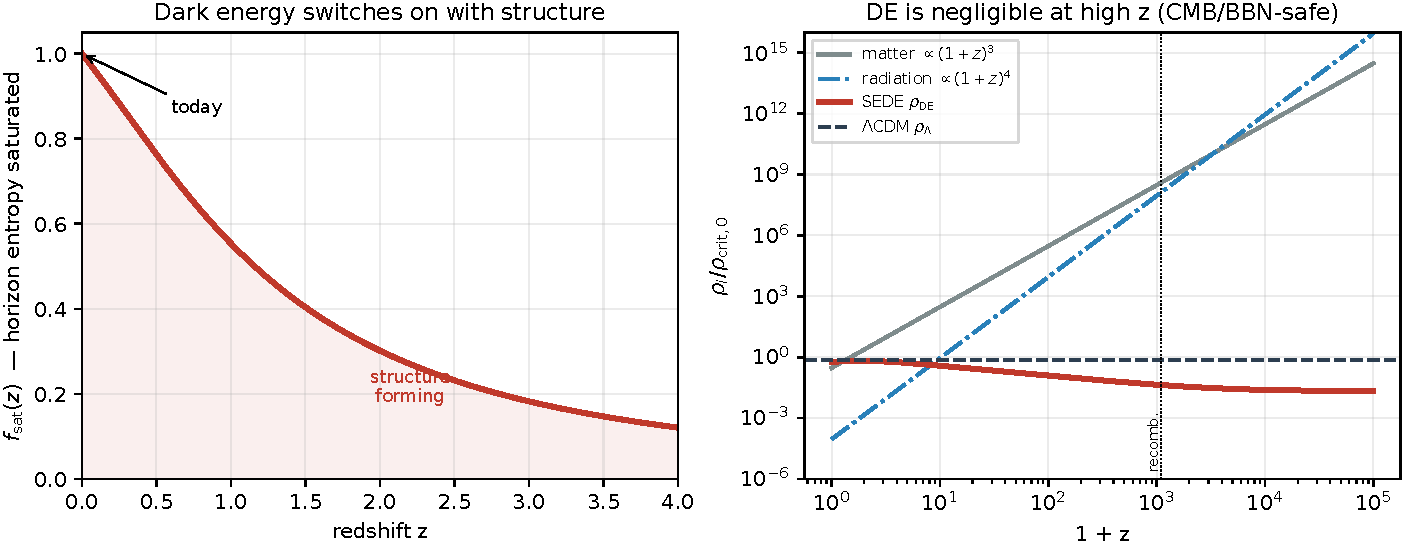
\includegraphics[keepaspectratio]{../../results/paper/fig1_mechanism}}
\caption{The mechanism. \emph{Left:} the effective activation fraction
(structure-growth gate) \(f_{\mathrm{sat}}(z)\) rises toward 1 today as
structure forms, activating the dark-energy gate --- the effective
running term \(\Lambda _{\mathrm{eff}} = 3\Omega _\mathrm{DE}0\) H
\(H_{0}\) \(f_{\mathrm{sat}}\) \emph{fades in} (computed from the
model's self-consistent linear growth factor D(z), §\ref{sec-2}).
\emph{Right:} the cosmic density inventory; SEDE's \(\rho _\mathrm{DE}\)
is orders of magnitude below matter and radiation at high z and falls
below \(\Lambda \mathrm{CDM}'s\) constant \(\rho _\Lambda\), so the
early universe (BBN, recombination) is standard --- the deformation acts
only on the late-time dark-energy fluid.}\label{fig:1}
\end{figure}

\begin{center}\rule{0.5\linewidth}{0.5pt}\end{center}

\section{Fixed inputs: why the dark sector adds no fitted
parameter}\label{sec-3}

In flat \(\Lambda \mathrm{CDM}\) the dark-energy amplitude
\(\Omega _\Lambda 0 = 1 - \Omega _{\mathrm{m}} - \Omega _{\mathrm{r}}\)
is itself fixed by the flatness closure, not an independent fit; SEDE
keeps exactly this --- no independent dark-energy amplitude beyond
flatness --- and differs only in that the \emph{redshift dependence} is
set by the horizon/growth prescription rather than held constant. What
that prescription fixes is the triplet \((\gamma\), w(z)-shape,
\(\lambda\)) plus the sound speed \(c_{\mathrm{s}}^{2}\) --- and each is
fixed by a stated theoretical choice (not fitted to cosmological data),
so SEDE adds no free dark-energy parameter. We are explicit about the
status of each choice below (some follow from flatness or the model
construction; others, notably \(\gamma\) and \(c_{\mathrm{s}}^{2}\), are
fixed prescriptions). The choices separate along the two scales of
§\ref{sec-2}. The magnitude of dark energy is the horizon scale, ∼
\(M_{\mathrm{P}}^{2}H^{2}\) ∼ \(\rho _{\mathrm{crit}}\) (the CKN bound
normalised by flatness, §\ref{sec-8-2}) --- not a fitted dark-sector
parameter. What the choices control is the \textbf{shape}: \emph{when}
and \emph{how sharply} that energy turns on. We therefore lead with the
structure coupling \(\gamma\) --- the shape, set by the binding energy
--- and then give \(w_{0}\), \(\lambda\), and \(c_{\mathrm{s}}^{2}\)
(Figure 2).

\subsection{\texorpdfstring{The structure coupling
\(\gamma  \approx  1.5\) from a halo-binding-energy derivation
(Prescription
4C)}{The structure coupling \textbackslash gamma  \textbackslash approx  1.5 from a halo-binding-energy derivation (Prescription 4C)}}\label{sec-3-1}

\(\gamma\) sets the sharpness of the structure gate, \(\gamma  = d\) ln
\(\Sigma _{\mathrm{S}} / d\) ln \(\sigma 8^{2}\) with
\(\Sigma _{\mathrm{S}}\) the entropy-weighted collapsed mass,
\(\Sigma _{\mathrm{S}}\)=∫ \(M^{p}\) (dn/d ln M) d ln M --- the
derivative is with respect to the variance \(\sigma 8^{2}\) because the
gate's argument is \(x = D^{2} = \sigma 8^{2}(z)/\sigma 8^{2}(0)\)
(§\ref{sec-3-4}, A.2); equivalently \(\gamma\)=½ d ln
\(\Sigma _{\mathrm{S}}/d\) ln \(\sigma 8\). The weight exponent p is
fixed by \emph{where} the structure-formation entropy is deposited ---
and the reservoir is fixed \emph{before any data enter}, by the model's
own §\ref{sec-2} identity. Because SEDE identifies
\(\rho _\mathrm{DE} = T_\mathrm{AH}\cdot s_{\mathrm{grav}}\)
(§\ref{sec-2}), \(f_{\mathrm{sat}}\) is by construction the
cosmic-\emph{horizon} entropy activation fraction (A.1), so the binding
energy released by virialisation is accounted in the horizon ledger at
its temperature \(T_\mathrm{AH} \propto  H\) --- \emph{not} the halo's
internal virial temperature \(T_{\mathrm{vir}} \propto  M^{2/3}\). With
\(T_\mathrm{AH}\) mass-independent at a fixed epoch, the Clausius
relation gives
\(\Delta S_\mathrm{AH} = E_{\mathrm{bind}}/T_\mathrm{AH} \propto  E_{\mathrm{bind}}\),
and the virial binding energy \(E_{\mathrm{bind}} \propto  M^{5/3}\)
then fixes p = 5/3. This reservoir choice follows from the §\ref{sec-2}
identity, and we state its history plainly rather than calling it
forced: an initial treatment used \(T_{\mathrm{vir}}\) (giving p = 1), a
reservoir error corrected for consistency with §\ref{sec-2}, not a
tuning --- but the correction is a discrete modelling revision, made
after the p = 1 mis-step. We flag the epistemic risk plainly: the
revision post-dates the p = 1 attempt and lands on the data-consistent
value, so --- absent a demonstrated microphysical transport channel
depositing the binding heat on the horizon (which we do not claim;
below) --- p = 5/3 is a prescription whose consistency with the data is
a check, not a uniquely forced output. What makes it more than post-hoc
is that the reservoir (horizon, \(T_\mathrm{AH}\), not virial
\(T_{\mathrm{vir}}\)) is fixed by the §\ref{sec-2} relation
independently of any fit; the residual freedom is whether that relation
is the right accounting, not the value of p given it.

\(\gamma\) has a transparent closed form. A self-similar reduction gives
\(\gamma  = (p - 1)\)⟨\(1/\alpha\)⟩\emph{\(\Sigma\)
\((\alpha  \equiv  -d\) ln \(\sigma /d\) ln M the effective spectral
slope, ⟨·⟩}\(\Sigma\) the entropy-weighted average), which reproduces
the full mass-function integral to 0.1\% (A.3) --- so the dark-sector
input is \emph{only} p = 5/3, with ⟨\(1/\alpha\)⟩ ordinary halo physics.
The \emph{numerical} \(\gamma\) then follows from a standard,
pre-specified halo model and inherits its systematics: a Sheth--Tormen
mass function over \(10^{10}\)--\(10^{16}\) \(M\odot\) with an EH98
transfer gives \(\gamma  = 1.50\) (Prescription 4C), and varying the
mass function (Press--Schechter, Tinker08, Despali16, Watson13), mass
range, and transfer function spans \(\gamma  \in  [1.14\), 1.60{]}
(median 1.50), dominated by the mass-range low-cutoff and robust
(1.48--1.57) to the mass-function and transfer choice. We therefore
claim precisely: the reservoir --- hence the weight p = 5/3 --- is fixed
by the model's own construction; the numerical \(\gamma  \approx  1.5\)
carries standard halo-model systematics of order ±0.2, none tuned to
cosmological data. That it lands near the diagnostic-fit value is then a
\emph{consistency check}, not the motivation. (We do not claim a
demonstrated microphysical transport channel depositing the binding heat
onto the horizon; the prescription is the accounting, and the smooth-DE
closure of §\ref{sec-3-4} ensures it induces no local dark-energy
perturbation.) Binding energy thus sets the gate \emph{shape}, not the
magnitude (§\ref{sec-2}, §\ref{sec-10} ledger).

\subsection{The equation of state w(z) from the fixed background,
conservation, and flatness}\label{sec-3-2}

The model has a single physical equation of state --- that of the
canonical fixed-point background (the boxed Friedmann equation of
§\ref{sec-2}), obtained from energy conservation,
\begin{equation}w(z) = -1 - \tfrac13\,\frac{d\ln\rho_{\rm DE}}{d\ln a},\end{equation} with
\(\rho _\mathrm{DE} = \Omega _\mathrm{DE}0\) \(\rho _{\mathrm{crit}}\),0
E \(f_{\mathrm{sat}}\) and the present-day normalisation fixed by
spatial flatness
\((\Omega _\mathrm{DE}0 = 1 - \Omega _{\mathrm{m}} - \Omega _{\mathrm{r}}\),
\(f_{\mathrm{sat}}(0) = 1\)). Evaluated on the self-consistent
background this gives \(w_{0} \approx  -1.0\), crossing \(-1\) at low
redshift \((z \approx  0.2)\) and dipping to \(\approx  -1.08\) by
\(z \approx  2\) --- DESI DR2's thawing/crossing quadrant. So w(z) is
fixed by \(\Omega _{\mathrm{m}}\) (through the background) with no free
EOS parameter; this is the w(z) used throughout (§\ref{sec-5}, Fig. 4).
\emph{(Convention: the literal present-day value is \(w(z=0) = -0.996\);
the reported pair \((w_{0}\), \(w_{\mathrm{a}}) \approx  (-0.98\),
−0.11) is the CPL projection of this same w(z) over 0 \textless{} z
\textless{} 1 --- the range used by the locked
\texttt{predictions.json}. The CPL \(w_{\mathrm{a}}\) steepens if fit
over a wider range, \(e.g. -0.17\) over 0 \textless{} z \textless{} 2,
so the fit window is quoted with the pair.)} Three \(w_{0}\) values
appear in this paper for \emph{different} objects; to avoid confusion:

\begin{longtable}[]{@{}
  >{\raggedright\arraybackslash}p{(\linewidth - 6\tabcolsep) * \real{0.2500}}
  >{\raggedright\arraybackslash}p{(\linewidth - 6\tabcolsep) * \real{0.2500}}
  >{\raggedright\arraybackslash}p{(\linewidth - 6\tabcolsep) * \real{0.2500}}
  >{\raggedright\arraybackslash}p{(\linewidth - 6\tabcolsep) * \real{0.2500}}@{}}
\toprule\noalign{}
\begin{minipage}[b]{\linewidth}\raggedright
object
\end{minipage} & \begin{minipage}[b]{\linewidth}\raggedright
scaling
\end{minipage} & \begin{minipage}[b]{\linewidth}\raggedright
role
\end{minipage} & \begin{minipage}[b]{\linewidth}\raggedright
\(w_{0}\)
\end{minipage} \\
\midrule\noalign{}
\endhead
\bottomrule\noalign{}
\endlastfoot
canonical SEDE & \(\rho _\mathrm{DE} \propto  H\) \(f_{\mathrm{sat}}\) &
the actual model & ≈ −1.0, crosses \(-1\) \\
\(\lambda =1\) ``temperature-factor'' variant & --- & closed-form
structural estimate (side note) & ≈ −0.85 \\
area-law branch & \(\rho _\mathrm{DE} \propto  H^{2}\)
\(f_{\mathrm{sat}}\) & disfavoured diagnostic alternative
(§\ref{sec-5-6}, §\ref{sec-8-1}) & ≈ −0.49 \\
\end{longtable}

Only the first row is the model's prediction; the \(-0.85\) is a sanity
check on the \(\Omega _{\mathrm{m}}\)-dependence (closed form
\(w_{0} = (4\Omega _{\mathrm{m}}/3 - 1)/(1 - \Omega _{\mathrm{m}})\))
and the \(-0.49\) is the \(\Delta =0\) alternative the data disfavour.

\subsection{\texorpdfstring{The H-coupling \(\lambda  = 0.5\) from the
horizon's volume
entropy}{The H-coupling \textbackslash lambda  = 0.5 from the horizon's volume entropy}}\label{sec-3-3}

\(\lambda\) fixes the \emph{magnitude}'s scaling with H, with no free
parameter: the gravitational entropy is taken to be the coarse-grained
entanglement entropy in the apparent-horizon volume,
\(S_{\mathrm{grav}} \propto  V_\mathrm{AH} \propto  R_\mathrm{AH}^{3}\),
i.e.~a \emph{constant} horizon entropy density. The conjugate
horizon-fluid ansatz
\((\rho _\mathrm{DE} = T_\mathrm{AH}\cdot s_{\mathrm{grav}}\),
\(T_\mathrm{AH} \propto  H\)) then gives
\(\rho _\mathrm{DE} \propto  H \equiv  H^{2\lambda }\) with
\(\lambda  = 1/2\) --- no deformation parameter. Equivalently, in the
Barrow language \(S = (A/A_{0})^{1+\Delta /2}\) this is the maximal
deformation \(\Delta  = 1\) \((s_\mathrm{AH} \propto  H^{1-\Delta }\),
\(\lambda  = 1-\Delta /2\)): the volume law \emph{is} \(\Delta =1\)
\((A^{3/2} = R^{3} = V)\). We keep \(\Delta\) only as a falsifiable test
of the volume law (its data measurement, §\ref{sec-5}/§\ref{sec-6}), not
as a model input; §\ref{sec-8} motivates the volume/space-filling state
(capping \(\Delta \leq 1\) and postulating saturation). (Verified
\(\Delta\)-free \(\equiv  \Delta =1\) bit-for-bit.)

\subsection{The perturbation sector: from a smooth-fluid closure to the
FPAB-SEDE cubic-KGB action}\label{sec-3-4}

SEDE's dark energy is \emph{background-growth-gated} (its
\(f_{\mathrm{sat}}\) depends on the growth history), which might suggest
it clusters with structure. The minimal treatment adopts a
\textbf{smooth-dark-energy closure}: \(f_{\mathrm{sat}}\) is a
functional of the background growth factor D(z) --- a function of cosmic
time only --- so the structure coupling is background-level / nonlocal /
coarse-grained, not local, \(\rho _\mathrm{DE}\) is homogeneous by
construction, and the dark energy has the standard metric-driven
response with \(c_{\mathrm{s}}^{2} = 1\). That closure is a
\emph{modelling} choice, not a theorem, and it is the sub-horizon
(\texttt{c\_s²=1}) limit of the completed theory rather than the theory
itself.

\textbf{The completed perturbation sector (FPAB-SEDE).} The background
\(\rho_X = \mu^3 H\,g(a)\) (with \(g\) the growth-shaped gate,
§\ref{sec-2}) admits a local, luminal \textbf{cubic
Kinetic-Gravity-Braiding} completion,
\(\mathcal{L} = M_{\rm P}^2 R/2 + K(X,\phi) - G_3(X,\phi)\,\Box\phi\),
whose finite (16-coefficient) action reproduces the background to
\(\max|\delta H/H| \approx 2\times10^{-4}\) over \(0 \le z \le 99\); we
call this completed effective theory \textbf{FPAB-SEDE} (fixed-point
activated braiding). This is a trajectory-level completion --- an
instance of designer / EFT-of-dark-energy reconstruction
\citep{Kennedy:2017sof, Gubitosi:2012hu, Gleyzes:2014dya} rather than a
symmetry-derived Lagrangian --- delivered in the stable \(\alpha\)-basis
\citep{Bellini:2014fua} to mochi-class
\citep{Cataneo:2024uox, Zumalacarregui:2016pph}, with braiding
\(\alpha_B = b\,\Omega_X\) the standard density-tracking ansatz and the
cubic-KGB no-ghost/no-gradient structure of
\citep{Deffayet:2011gz, Kobayashi:2011nu}. Because it carries no
\(G_4/G_5\) term, \(\alpha_M = \alpha_T = 0\) and \(c_T = 1\) exactly
(GW170817-safe). This is a \emph{derived} statement, not merely an EFT
prior: an exact all-orders-in-the-tensor-perturbation expansion of the
FPAB action shows that \(K\) and \(G_3\) contribute nothing to the
quadratic tensor action for arbitrary functional forms, so the entire
tensor sector is that of GR and the GW and EM luminosity distances
coincide (\(\Xi_0 = 1\) exactly) --- see the tensor-sector and
standard-siren predictions in §\ref{sec-6} (script
\texttt{fpab\_tensor\_sector.py}). Its perturbations are solved
\emph{dynamically} (Mochi-CLASS, not a PPF or an imposed sound speed):
ghost- and gradient-stable, with
\begin{equation}c_s^2 \in [0.018,\,0.18],\qquad \gamma_{\rm slip}=1,\qquad \mu_\infty(0)=1.05,\end{equation}
i.e.~\textbf{unit gravitational slip and a ∼5\% near-horizon
scalar-force enhancement} that turns on across \(k_{50} = 0.70\,aH\) to
\(k_{90} = 2.1\,aH\) --- a scale-dependent \(\mu(k,z)\), \emph{not} a
smooth \(c_s^2=1\) fluid. The earlier \(c_s^2=1\) ``smooth dark energy''
statement is thus the sub-horizon limit of this result, and the
marginalised fit of §\ref{sec-5} (run in that PPF limit) is valid at the
background/distance level while the growth-side observables are revised
to the FPAB values below and treated as forecasts pending a full
perturbative refit (§\ref{sec-5}, §\ref{sec-6}).

\begin{longtable}[]{@{}
  >{\raggedright\arraybackslash}p{(\linewidth - 4\tabcolsep) * \real{0.3333}}
  >{\raggedright\arraybackslash}p{(\linewidth - 4\tabcolsep) * \real{0.3333}}
  >{\raggedright\arraybackslash}p{(\linewidth - 4\tabcolsep) * \real{0.3333}}@{}}
\toprule\noalign{}
\begin{minipage}[b]{\linewidth}\raggedright
input
\end{minipage} & \begin{minipage}[b]{\linewidth}\raggedright
value
\end{minipage} & \begin{minipage}[b]{\linewidth}\raggedright
status --- fixed by
\end{minipage} \\
\midrule\noalign{}
\endhead
\bottomrule\noalign{}
\endlastfoot
\(\lambda\) (H-coupling) & 0.5 & postulate --- volume-law horizon
entropy \(S_{\mathrm{grav}} \propto  V_\mathrm{AH}\) \((\)≡ Barrow
\(\Delta =1\)), §\ref{sec-3-3}, §\ref{sec-8} \\
w(z) (EOS) & \(w_{0} \approx  -1.0\), crosses \(-1\) & derived ---
spatial flatness + the boxed closure equation (§\ref{sec-2}),
§\ref{sec-3-2} (no free EOS parameter) \\
\(\gamma  / gate\) q & ≈ 1.50; gate \(q = \sigma_R^2(a)\), R = 8
\(h^{-1}Mpc\) & fixed prescription --- halo-binding weighting
(§\ref{sec-3-1}); the model-owned filtered variance replaces the
abstract \(D^{2}\) \\
perturbations & \(c_s^2 \in [0.018,0.18]\), \(\gamma_{\rm slip}=1\),
\(\mu_\infty=1.05\) & \textbf{computed} --- FPAB-SEDE cubic-KGB action +
Mochi-CLASS (§\ref{sec-3-4}); \(c_s^2=1\) is the sub-horizon limit \\
\end{longtable}

\begin{figure}
\centering
\pandocbounded{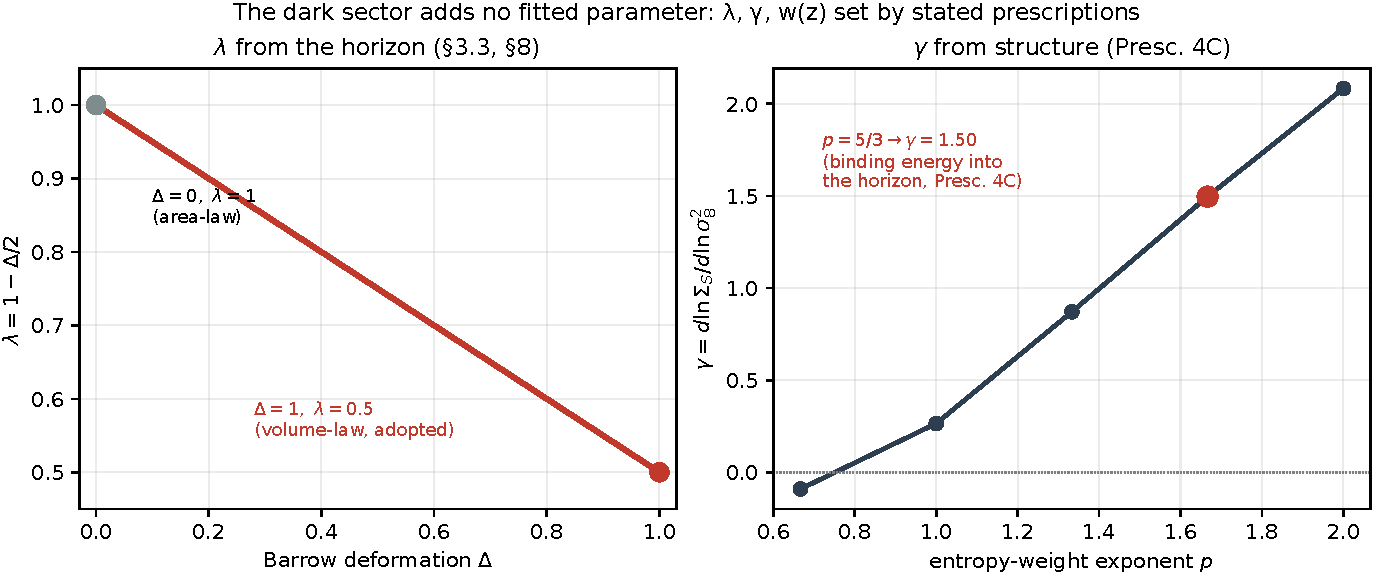
\includegraphics[keepaspectratio]{../../results/paper/fig2_inputs}}
\caption{The two fixed dark-sector couplings. \emph{Left:} the
H-coupling \(\lambda = 1 - \Delta /2\) as a function of the Barrow
deformation; the volume-law endpoint \(\Delta = 1\) (the postulate of
§\ref{sec-8}) fixes \(\lambda = 0.5\). \emph{Right:} the structure
coupling \(\gamma = d\) ln \(\Sigma _{\mathrm{S}}/d\) ln
\(\sigma 8^{2}\) (variance convention, §\ref{sec-3-1}) as a function of
the entropy-weight exponent p; the binding-energy-into-the-horizon
argument (Prescription 4C, A.3) fixes p = 5/3, giving \(\gamma = 1.50\)
--- close to the value favoured in diagnostic fits. Neither is a fitted
parameter.}\label{fig:2}
\end{figure}

\begin{center}\rule{0.5\linewidth}{0.5pt}\end{center}

\section{Data and analysis methodology}\label{sec-4}

\subsection{Data}\label{sec-4-1}

We use a standard late-time-plus-compressed-CMB compilation, with both
models fit to the identical data vector: - \textbf{BAO:} DESI DR2
(galaxy, QSO, and \(Ly\alpha\) tracers, z = 0.3--2.33), as
\(D_{\mathrm{M}}/r_{\mathrm{d}}\) and \(D_{\mathrm{H}}/r_{\mathrm{d}}\).
- \textbf{Supernovae:} Pantheon+ as the baseline, with DES-5YR and
Union3 used independently for the robustness cross-check of
§\ref{sec-5-4}. - \textbf{Cosmic chronometers:} the Moresco et al.~H(z)
compilation (model-independent expansion rates). -
\textbf{Redshift-space distortions:} the Gold-2018
\citep{Sagredo:2018ahx} \(f\sigma 8(z)\) growth compilation (a standard,
vetted set chosen for comparability with prior growth analyses;
combining it with DESI DR2 BAO follows common late-time practice, and
the audit below corrects a few mis-entered points), with the data audit
of Appendix~\ref{sec-C} (a small number of mis-entered points corrected
to their published values). - \textbf{CMB:} the compressed Planck
distance priors (shift parameter R, acoustic scale \(l_{\mathrm{A}}\),
\(\omega _{\mathrm{b}}\)), with the full \(plik_{\mathrm{lite}}\)
likelihood used as a cross-check. - \textbf{Local distance ladder:} the
SH0ES \(H_{0}\) prior. - \textbf{Out-of-sample (§\ref{sec-5-3}):} the
pre-DESI eBOSS DR16 full-shape BAO, held entirely out of the main fit.

\subsection{CAMB-in-the-loop: a physical sound horizon}\label{sec-4-2}

The single most important methodological point is that the sound horizon
is not a free parameter. Earlier exploratory fits that floated
\(r_{\mathrm{d}}\) found large apparent preferences for SEDE; those did
not survive a physical sound horizon. Here, at every point in the chain,
\(r_{\mathrm{drag}}\), \(r_{\mathrm{star}}\), and \(\theta\)* are
computed self-consistently from the background by CAMB
(``CAMB-in-the-loop''), so the BAO and CMB distances are tied to the
same early-universe physics for both models. This is what makes the
\(\Delta \mathrm{DIC}\) of §\ref{sec-5} a like-for-like comparison
rather than an artifact of a free standard ruler. The CMB enters as the
compressed (R, \(l_{\mathrm{A}}\)) distances computed on the SEDE
background through the same CAMB call. \emph{Scope of the compressed
likelihood, and its full-likelihood validation:} the compressed priors
capture the background distance to last scattering (and hence the
early-dark-energy fraction that drives the \(\Delta\) leverage of
§\ref{sec-5-6}), but not the full acoustic-peak/polarisation or
lensing/ISW information. We therefore validate the headline against the
full primary CMB likelihood: a CAMB-in-the-loop fit on the full Planck
\(plik_{\mathrm{lite}}\) \(\mathrm{TTTEEE} + low\ell\) TT/EE, with the
five cosmological parameters and the Planck nuisance \emph{all free},
gives \(\Delta \chi ^{2}(\mathrm{SEDE}-\Lambda \mathrm{CDM}) = -0.43\)
--- the preference sitting in the high-ℓ peak structure \((-0.37)\),
\emph{negative} (mildly favouring SEDE), not the large positive
\(\Delta \chi ^{2}\) that the holographic-DE early--late tension would
produce (§\ref{sec-5-1}, §\ref{sec-9}). This directly tests the
acoustic-peak channel the compression omits, and we have confirmed it
against the full non-lite plik with all 15 foregrounds sampled
\((\Delta \chi ^{2} = -0.33\), consistent with the lite \(-0.43\);
§\ref{sec-9}). \emph{Stated scope of what remains:} only the ACT DR6
\emph{primary} multifrequency likelihood is not run (ACT \emph{lensing},
the DE-sensitive channel, is, evaluated at the primary best-fit;
§\ref{sec-5-1}). It is formally deferred under a pre-registered trigger
(pre-registration §\ref{sec-E}): the \texttt{act\_dr6\_mflike}
likelihood and its multi-GB data products are not installed, and with
three concordant CMB datasets --- \(plik_{\mathrm{lite}}\), full
non-lite plik, and ACT DR6 lensing --- all at
\textbar{}\(\Delta \chi ^{2}\)\textbar{} \textless{} 1 (these are not
the same estimator: the \(plik_{\mathrm{lite}}/non\)-lite numbers are
\emph{profiled} over the cosmological and nuisance parameters, whereas
the ACT-lensing value is a \emph{single-point} evaluation at the primary
best-fit --- so their numerical closeness is corroborative but not a
like-for-like concordance, and the full \emph{marginalised} CMB analysis
is the companion paper's, §5.1), a fourth primary likelihood is not
expected to overturn them; the committed (falsifiable) expectation is
\textbar{}\(\Delta \chi ^{2}(\mathrm{SEDE}-\Lambda \mathrm{CDM})\)\textbar{}
\textless{} 1, a large positive value being a genuine failure. The
\%-level metric effects (§\ref{sec-4-4}) are reported but not used in
the headline fit.

\subsection{Inference and model comparison}\label{sec-4-3}

Parameters are sampled by MCMC, marginalising over
\(\Omega _{\mathrm{m}}\), \(H_{0}\) (with the SH0ES prior),
\(\omega _{\mathrm{b}}\), the \(amplitude/\sigma 8\), and
\(r_{\mathrm{d}}\)-determining physics --- the same five for SEDE and
\(\Lambda \mathrm{CDM}\), since SEDE's dark sector is fixed
(§\ref{sec-3}). Model comparison uses the deviance information criterion
(DIC), which penalises the effective number of parameters
\(p_{\mathrm{D}}\). The marginalised chains give
\(p_{\mathrm{D}} = 4.8\) (SEDE) and 4.9 \((\Lambda \mathrm{CDM})\) ---
nearly equal \((\Delta p_{\mathrm{D}} \approx  0.1)\), as expected since
the two share the same five fitted parameters --- so
\(\Delta \mathrm{DIC}\) reduces essentially to the \(\chi ^{2}\)
difference: \(\Delta \mathrm{DIC} = -4.69\) (Barrow preferred); the
chains' \(\Delta \chi ^{2}_{\mathrm{min}} = -4.66\) agrees with the
\(optimiser's -4.68\) to sampling precision. With k = 5 fitted
parameters for \emph{both} models \((\Delta k = 0)\),
\(\mathrm{AIC} = \chi ^{2} + 2k\) and \(\mathrm{BIC} = \chi ^{2} + k\)
ln N (N = 1628) give
\(\Delta \mathrm{AIC} = \Delta \mathrm{BIC} = \Delta \chi ^{2} = -4.68\)
\((-3.17\) for the full-CMB joint --- this paper's own CAMB-in-the-loop
fold-in on the wider data vector; the companion's independent
mochi-class best-fit on DESI+SN+Planck is a related \(-3.4\)) --- but
the AIC/BIC coincidence is a tautology, not an independent cross-check:
at \(\Delta k = 0\) the AIC and BIC penalties cancel \emph{identically},
so the criteria carry no information beyond \(\Delta \chi ^{2}\) and are
silent on the model's \emph{form}-flexibility (which only the
§\ref{sec-5-2} bootstrap addresses). We also compute a Bayesian
evidence. A Laplace estimate (ln
\(B\)≈½\(\Delta \chi ^{2}_{\mathrm{min}} - ln\) Occam, with ln
\(Occam \approx  0\) for the identical \(\Delta k = 0\) prior) gives ln
\(B(\mathrm{SEDE}-\Lambda \mathrm{CDM}) \approx  +2.3\) ---
\emph{moderate} on the Jeffreys/Kass--Raftery scale, favouring SEDE;
with the contested SH0ES prior dropped it falls to ln
\(B \approx  +1.4\) (½ × 2.89), still \emph{positive} but weaker, so
roughly 40\% of the evidence is carried by SH0ES and the rest by the CMB
distance (§\ref{sec-5-4} ii′). (A full nested-sampling re-run at the
updated best-fit is deferred to the companion; the Laplace value is
reliable here because \(\Delta k = 0\) makes the Occam term vanish.)
Significance is then assessed not by any single criterion but by the
false-preference calibration of §\ref{sec-5-2}.

\subsection{Perturbations: the FPAB-SEDE cubic-KGB completion, solved
dynamically}\label{sec-4-4}

The marginalised analysis of §\ref{sec-5} uses the sub-horizon
smooth-fluid limit (PPF, \(c_{\mathrm{s}}^{2} = 1\), the \(w = -1\)
crossing handled by the crossing prescription), which is adequate for
the background/distance inference. The \emph{completed} perturbation
sector is the FPAB-SEDE cubic-KGB action (§\ref{sec-3-4}), solved
dynamically in Mochi-CLASS --- not PPF and not an imposed sound speed.
It is ghost/gradient-stable with \(c_{\mathrm{T}} = 1\),
\(\gamma_{\rm slip}\) = 1, \(c_{\mathrm{s}}^{2} \in  [0.018\), 0.18{]},
and a scale-dependent effective coupling \(\mu (k\),z) turning on near
the horizon (\(\mu_\infty(0)\) = 1.05, \(k_{50}\) = 0.70 aH). At fixed
primordial normalisation it gives \(\sigma 8(0) = 0.811\) and
\(f\sigma 8(0) = 0.422\) --- \emph{raising} growth by \(\approx  3\)\%
relative to matched \(\Lambda \mathrm{CDM}\) \((\sigma 8 = 0.800)\),
with CMB-lensing \(C_\ell ^{\phi \phi }\) ratios \(\approx  1.02\)--1.03
--- a mild lensing enhancement that the companion tests against the
direct Planck 2018 lensing reconstruction \citep{Planck:2018lbu}, whose
amplitude sits near unity (unlike the peak-smoothing
\(A_{\mathrm{lens}} > 1\) \citep{Motloch:2018pjy, Addison:2023fqc}).
These growth-side numbers supersede the earlier smooth-fluid values
\((\sigma 8 \approx  0.76)\) and are reported as \textbf{fixed-parameter
forecasts}: they have not been jointly refit with the standard and
nuisance parameters (a fixed-parameter diagonal CMB-TT screen gives
\(\Delta \chi ^{2} \approx  52\) through ℓ = 1800, which is \emph{not} a
constraint but a demonstration that the full perturbative likelihood
must be re-marginalised).

\section{Results}\label{sec-5}

\subsection{The joint fit and the equation of state}\label{sec-5-1}

In the marginalised joint analysis, SEDE is moderately preferred over
\(\Lambda \mathrm{CDM}\), with a deviance information criterion
difference \(\Delta \mathrm{DIC} \approx  -4.7\) in SEDE's favour.
Because the dark sector adds no fitted parameter (§\ref{sec-3}), the two
models share the same five parameters and near-identical effective
complexity (measured \(p_{\mathrm{D}} = 4.8\) vs 4.9; §\ref{sec-4-3}):
the preference is in fit, not bought with parameters. The headline
survives the full primary CMB likelihood, not only the compressed
priors: a profiled CAMB-in-the-loop fit on the full Planck
\(plik_{\mathrm{lite}}\) \(\mathrm{TTTEEE} + low\ell\) gives
\(\Delta \chi ^{2}(\mathrm{SEDE}-\Lambda \mathrm{CDM}) = -0.43\) ---
mildly favouring SEDE, not the large positive \(\Delta \chi ^{2}\) the
standard holographic-DE early--late tension would produce (the full
decomposition and red-team are in §\ref{sec-4-2} and §\ref{sec-9}).
Folding the full primary CMB \emph{into} the joint leaves the preference
intact: joint
\(\Delta \chi ^{2}(\mathrm{SEDE}-\Lambda \mathrm{CDM}) = -3.17\)
\((\Lambda \mathrm{CDM}\) 2443.99 → SEDE 2440.83). The full
acoustic-peak likelihood thus retains about two-thirds of the
compressed-prior preference \((-3.17\) vs \(-4.68\)); we treat the
full-likelihood value as the conservative anchor, and note that the mock
calibration of §\ref{sec-5-2} applies to the \emph{compressed} pipeline
--- against that null, −3.17 corresponds to ∼\(2.4\sigma\) (Gaussian),
at the edge of the sampled draws rather than beyond them. SEDE is
preferred either way, so the preference is not an artifact of the CMB
compression, but the quoted significance band (§\ref{sec-5-2}) spans the
two pipelines. The definitive full-likelihood analysis --- DESI DR2 BAO
+ Pantheon+ + full Planck 2018 \((low\ell\)
\(\mathrm{TT} + plik_{\mathrm{lite}}\) TTTEEE) driven through the
modified-gravity Boltzmann code, with converged MCMC chains --- is
carried out in the companion paper \citep{Pandev:2026obstest}, which
finds a marginalised \(\Delta \mathrm{DIC} = -3.5\) (full primary CMB;
robust part \(\Delta\)⟨\(\chi ^{2}\)⟩ ≈ −3.0) that it reads, SH0ES-free,
as statistically consistent with \(\Lambda \mathrm{CDM}\) with a mild
same-direction pull --- further eroded to \(-2.3\) in a full
BAO/SN/BBN-anchored joint refit once the companion folds in the direct
Planck lensing \((\phi \phi )\) datum (about a third of the high-ℓ gain
is consistent with the absorbed \(A_{\mathrm{lens}}\) systematic) ---
the conservative anchor of, and consistent with, the compressed-CMB
preference here; the reader seeking the full parameter posteriors and
the growth predictions \((f\sigma 8\), ISW) should consult it. The
physical reason the CMB poses no obstacle is that SEDE carries
\emph{less} early dark energy than \(\Lambda \mathrm{CDM}\) and deforms
only the late-time expansion (Figure 5): there is no early--late wall of
the kind that disfavours standard holographic DE. The recovered
background parameters are physical and close to \(\Lambda \mathrm{CDM}\)
\((\Omega _{\mathrm{m}} \approx  0.30\), \(H_{0} \approx  68.9\)).
\emph{(The structure amplitude is revised upward to
\(\sigma 8(0) = 0.811\) by the completed FPAB theory --- it }raises*
growth, so the earlier smooth-fluid \(\sigma 8 \approx  0.76\) and any
S8-easing claim are retracted; §\ref{sec-4-4}, §\ref{sec-9}.)* The
absolute \(\chi ^{2}/dof \approx  0.88\) (SEDE 1436.1/1628;
§\ref{sec-5-5}) is dominated by the well-fit Pantheon+ SN (the BAO and
SN residuals are shown in Figure 3) and is \emph{not} a goodness-of-fit
probability for this heterogeneous, partly-compressed compilation with a
marginalised SN nuisance; we use only matched-model differences
\((\Delta \mathrm{DIC}\), \(\Delta \chi ^{2}\)) on the identical data
vector for inference. The canonical \((\lambda  = 1/2)\) equation of
state crosses \(w = -1\), with a present-day value near \(-1\) and a dip
to \(\approx  -1.08\) by \(z \approx  2\), i.e.~\((w_{0}\),
\(w_{\mathrm{a}}) \approx  (-0.98\), −0.11) --- squarely in DESI DR2's
evolving-dark-energy (thawing/crossing) quadrant, ∼\(2.7\sigma\) from
the DESI DR2 preferred (evolving-DE) point but only ∼\(0.5\sigma\) from
\(\Lambda \mathrm{CDM}\) \((-1\), 0) --- so the EOS \emph{shape} does
not by itself separate SEDE from \(\Lambda \mathrm{CDM}\) (only the
deformation \(\Delta\) does, §\ref{sec-6}), and SEDE is disfavoured
\emph{alongside} \(\Lambda \mathrm{CDM}\) if the steep DESI signal firms
up. (These two statements --- ∼\(0.5\sigma\) from
\(\Lambda \mathrm{CDM}\) in the projected EOS, yet
\(\Delta \mathrm{DIC} \approx  -4.7\) over \(\Lambda \mathrm{CDM}\) ---
are compatible because the \((w_{0}\), \(w_{\mathrm{a}}\)) projection is
not the statistic the data weigh: the preference is carried by the
integrated distance to last scattering and the \(H_{0}\) calibration
(§\ref{sec-5-4}), where SEDE's small but coherent low-z deformation of
E(z) accumulates, not by the local EOS shape; and the no-SH0ES run
(§\ref{sec-5-4} ii′) shows the CMB-distance gain persists when \(H_{0}\)
is released downward, so the effect is not reducible to an \(H_{0}\)
accommodation.) The crossing is not imposed; it is where the expansion
term and the horizon-entropy-production term in 1 + w balance (Result
13, §\ref{sec-6}).

\begin{figure}
\centering
\pandocbounded{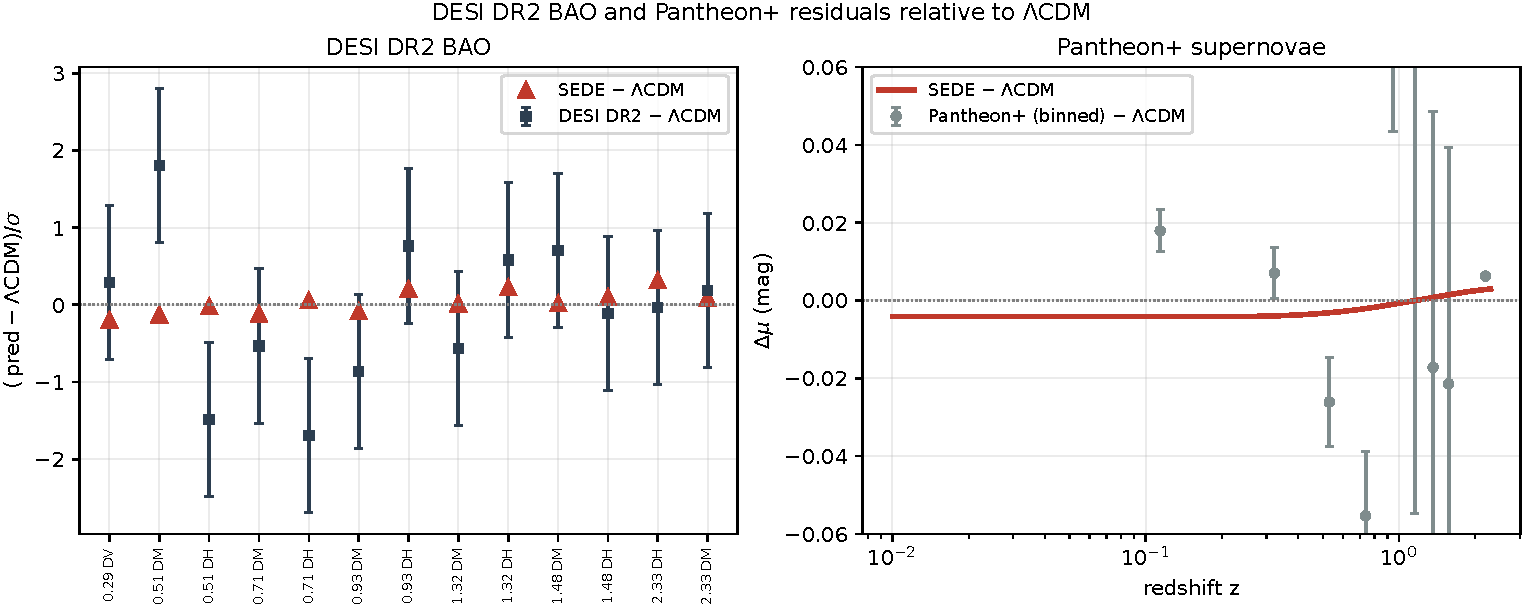
\includegraphics[keepaspectratio]{../../results/paper/fig3_datafit}}
\caption{Matched residual comparison (relative to
\(\Lambda \mathrm{CDM}\)). \emph{Left:} DESI DR2 BAO residuals relative
to the \(\Lambda \mathrm{CDM}\) best fit, in units of \(\sigma\) --- the
data (slate) with the SEDE prediction (red); SEDE is consistent with the
measurements and sits between \(\Lambda \mathrm{CDM}\) and the points
that pull away from it. \emph{Right:} Pantheon+ supernova residuals
(binned) versus \(\Lambda \mathrm{CDM}\), with the SEDE shape
overplotted. SEDE and \(\Lambda \mathrm{CDM}\) are close at present
precision; the preference is carried by the CMB-distance and \(H_{0}\)
channels (§\ref{sec-5-4}), not by the BAO/SN data shown
here.}\label{fig:3}
\end{figure}

\begin{figure}
\centering
\pandocbounded{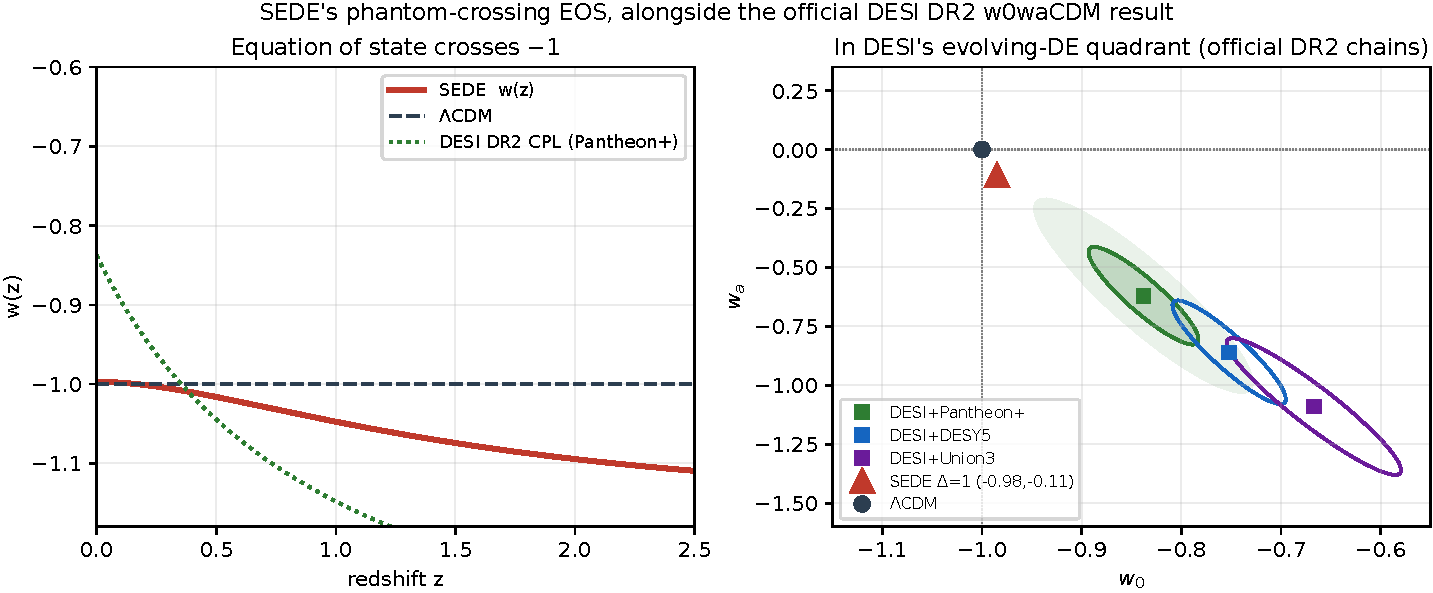
\includegraphics[keepaspectratio]{../../results/paper/fig4_eos}}
\caption{The equation of state. \emph{Left:} the canonical SEDE-H fluid
w(z) (red) crosses \(-1\) near \(z \approx 0\) and dips into the phantom
regime \((\approx -1.08\) by \(z \approx 2\)), the same sense as DESI
DR2's CPL fit (green) and distinct from \(\Lambda \mathrm{CDM}\)
(dashed). \emph{Right:} the \((w_{0}\), \(w_{\mathrm{a}}\)) plane ---
SEDE sits between \(\Lambda \mathrm{CDM}\) and the DESI DR2 w0waCDM
contour, in the evolving-dark-energy quadrant. The crossing is not
imposed; it is where the expansion and horizon-entropy-production terms
in 1 + w balance (Result 13).}\label{fig:4}
\end{figure}

\begin{figure}
\centering
\pandocbounded{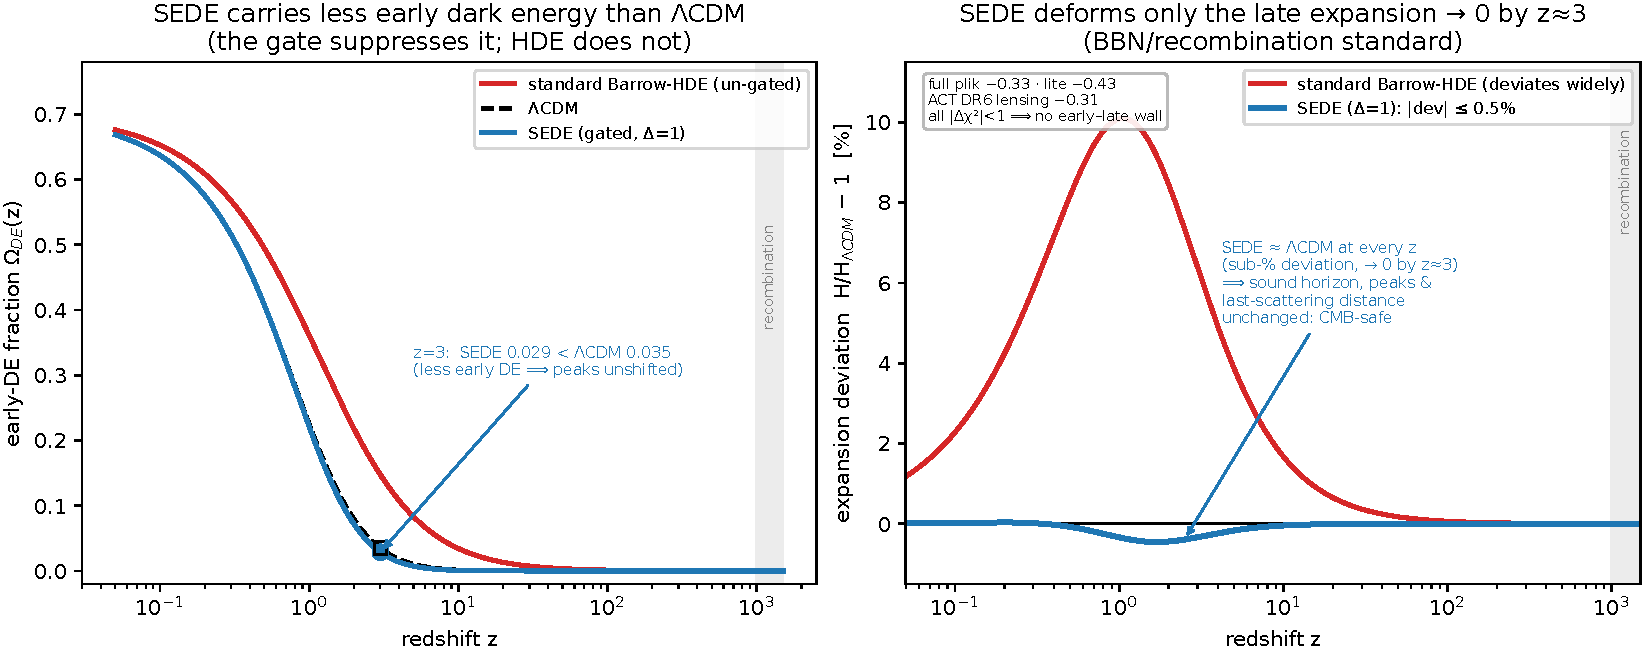
\includegraphics[keepaspectratio]{../../results/fig_cmb_earlyde}}
\caption{Why SEDE survives the CMB where standard holographic dark
energy does not --- the physical content of the full-CMB result (full
non-lite plik \(\Delta \chi ^{2} = -0.33\),
\(plik_{\mathrm{lite}} -0.43\), ACT DR6 lensing \(-0.31\); all
\textbar{}\(\Delta \chi ^{2}\)\textbar{} \textless{} 1). \emph{Left:}
the early-dark-energy fraction \(\Omega _\mathrm{DE}(z)\). SEDE's
structure gate \((f_{\mathrm{sat}}\) → 0 at high z) holds it
\emph{below} \(\Lambda \mathrm{CDM}\)
\((\Omega _\mathrm{DE}(z=3) = 0.029 < 0.035\) at
\(\Omega _{\mathrm{m}} = 0.30\)), whereas un-gated standard Barrow-HDE
carries substantially more early DE --- the runaway that drives the
early--late tension of refs. {[}\citep{Wu:2025vfs}{]}. \emph{Right:} the
fractional expansion deviation \(H/H_\Lambda \mathrm{CDM} - 1\). SEDE's
deviation is sub-percent and confined to \(z \lesssim 3\), decaying to
zero through BBN and recombination, so the sound horizon, the
acoustic-peak positions, and the distance to last scattering are all
essentially unchanged; standard Barrow-HDE deviates over a far wider
range. SEDE has \emph{less} early dark energy than
\(\Lambda \mathrm{CDM}\), not more --- hence no early--late
wall.}\label{fig:5}
\end{figure}

\subsection{Is the preference real, or model
flexibility?}\label{sec-5-2}

A \(\Delta \mathrm{DIC} \approx  -4.7\) is moderate but not, on its own,
decisive --- and a structure-gated model could in principle be winning
by flexibility rather than by capturing a real signal. We test this
directly with a false-preference calibration (a parametric bootstrap).
We generate mock datasets from a \(\Lambda \mathrm{CDM}\) truth ---
re-drawing \emph{every} probe self-consistently, crucially including the
compressed CMB distances (R, \(l_{\mathrm{A}}\)) and the SH0ES prior,
not just the late-time data --- and refit both models to each mock.
Under \(\Lambda \mathrm{CDM}\) truth a flexible model would still tend
to ``win''; SEDE does not: the null distribution of
\(\Delta \chi ^{2}(\mathrm{SEDE} - \Lambda \mathrm{CDM})\) is centred
near zero (2000-mock run: mean +0.61, s.d. 1.59; SEDE if anything fits
\(\Lambda \mathrm{CDM}\)-truth mocks slightly \emph{worse}, consistent
with having no spare flexibility). The real data give
\(\Delta \chi ^{2} = -4.68\), beyond \emph{every} one of the 2000 null
draws (the most SEDE-preferring mock reached only \(-4.44\)): 0/2000, p
\textless{} 0.0015 (Clopper--Pearson 95\% upper limit, i.e.~an
empirically guaranteed \(> 2.9\sigma\)). A Gaussian read-off of the null
(mean +0.61, s.d. 1.59) places the real value at \(z \approx  -3.3\)
(∼\(3.3\sigma\)), now consistent with --- rather than extrapolating
beyond --- the direct empirical bound; the 2000-mock run therefore
resolves the calibrated significance at ∼\(3\sigma\), empirically
anchored rather than tail-extrapolated. Rerun with the contested SH0ES
prior removed from both the real fit and the mocks, the real value moves
to \(\Delta \chi ^{2} = -2.89\) and the calibration weakens to
∼\(2.3\sigma\) --- degraded but still beyond most of the null, now
carried by the CMB-distance channel (§\ref{sec-5-4} ii′).

One caveat stands. The significance is
\textbf{CMB-distance-treatment-dependent}: an initial version of this
test held the CMB distances \emph{fixed} across mocks, which biased the
null (mean → −2.9, coincident with the then-current real value) and made
the preference look like pure flexibility \((p \approx  0.5\) in that
version). The fixed-CMB variant is not a defensible null --- it deletes
the CMB-distance scatter the real analysis is exposed to --- so the
re-drawn procedure is correct on prior grounds, not selected post hoc. A
different \(l_{\mathrm{A}}/\mathrm{CAMB}\) handling shifts the
significance by up to ∼\(1\sigma\), and the one independent-pipeline
cross-check on record (run against the pre-revision real value;
Appendix~\ref{sec-D}) recovered the preference at ∼\(2\sigma\). The
honest band is therefore ∼2--\(3\sigma\) across pipelines, with
∼\(3\sigma\) the fiducial-pipeline significance (now empirically
anchored by the 2000-mock null), pending independent reproduction.

\begin{figure}
\centering
\pandocbounded{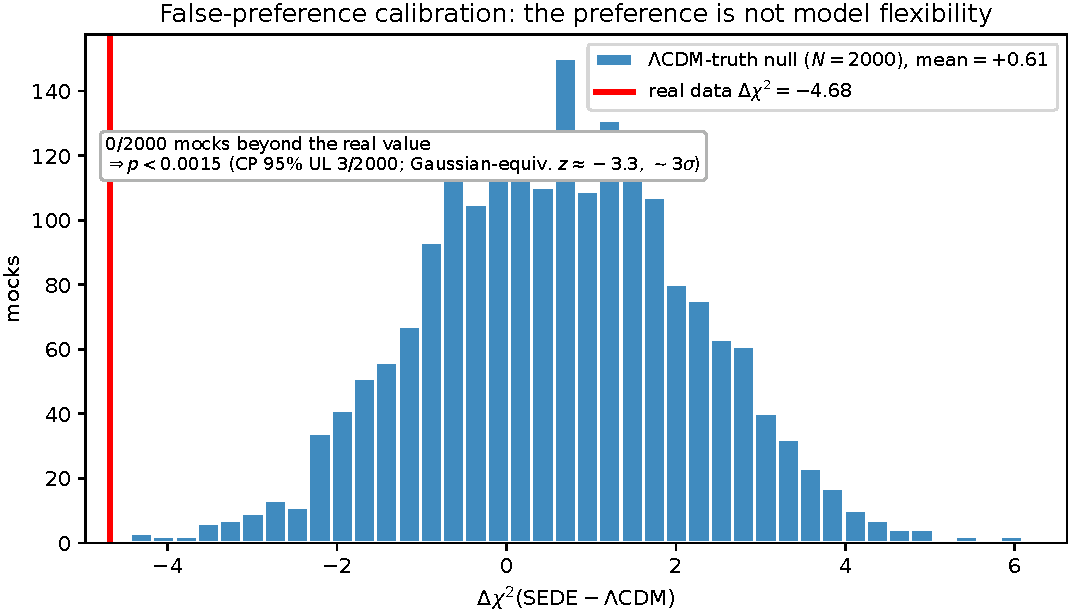
\includegraphics[keepaspectratio]{../../results/fig_F5_calibration}}
\caption{The false-preference calibration. Histogram: the null
distribution of
\(\Delta \chi ^{2}(\mathrm{SEDE} - \Lambda \mathrm{CDM})\) from
\(\Lambda \mathrm{CDM}\)-truth mocks (all probes, including the
compressed CMB and SH0ES, re-drawn self-consistently), centred near zero
(2000-mock mean +0.61) --- SEDE has no flexibility advantage under
\(\Lambda \mathrm{CDM}\) truth. Red line: the real data,
\(\Delta \chi ^{2} = -4.68\), beyond \emph{every} null draw. In the
2000-mock run 0 mocks are as SEDE-preferring as the real data (0/2000, p
\textless{} 0.0015, ∼\(3\sigma\)); the preference is not attributable to
flexibility.}\label{fig:6}
\end{figure}

\subsection{Out-of-sample check}\label{sec-5-3}

A further check against a flexibility explanation is out-of-sample
prediction. We trained SEDE on real pre-DESI data only (eBOSS DR16
full-shape BAO, LRG/QSO) and used it to predict the later, held-out DESI
DR2 BAO: in this split SEDE matches the held-out DESI DR2 trend better
than \(\Lambda \mathrm{CDM}\) by \(\Delta \chi ^{2} = -8.56\) (Figure
7); a low-z→high-z split of the same kind gives \(-10.45\). A model
winning purely by flexibility would tend to do \emph{worse} out of
sample, so this is encouraging --- i.e.~a pre-DESI-trained SEDE
realisation predicts the DESI DR2 trend in this split. \emph{Two
clarifications so this number is read correctly.} (a) Not comparable to
the in-sample \(\Delta \mathrm{DIC}\) --- and the reason is instructive.
\(The -8.56\) is the \(\Delta \chi ^{2}\) on the held-out DESI BAO
subset alone at fixed pre-DESI-trained parameters, whereas the in-sample
\(\Delta \chi ^{2} = -4.68\) is the net over the full 1628-point
compilation with all parameters free. The sharp point is that the
\emph{same} DESI BAO probe contributes only \(-0.29\) in-sample (the
probe decomposition, §\ref{sec-5-4}) yet \textbf{−8.56 out-of-sample}:
in the joint fit the shared geometric parameters
\((\Omega _{\mathrm{m}}\), \(H_{0}\), \(r_{\mathrm{d}}\)) \emph{absorb}
the BAO information, so the residual model difference on DESI BAO
collapses (the preference re-surfaces in the CMB-distance \(+ H_{0}\)
channels, §\ref{sec-5-4}); out of sample those parameters are pinned by
\emph{other} data and cannot be tuned to the held-out BAO, so SEDE's
evolving-w(z) \emph{shape} --- calibrated where it never saw DESI ---
must predict it, and does so better than \(\Lambda \mathrm{CDM}'s\)
constant-\(\Lambda\) shape. The gap between \(-0.29\) (post-absorption)
and \(-8.56\) (pre-absorption) is therefore the fingerprint of a shape
difference that generalises, the opposite of over-fitting (which pushes
OOS the other way), not an anomaly. (b) \textbf{Direction-dependent.}
The signal lives in the low-z → high-z direction (the DESI evolving-DE
direction, \(\Delta \chi ^{2} = -10.45\)); the reverse split (high-z →
low-z) is flat and marginally favours \(\Lambda \mathrm{CDM}\) (+0.27),
so part of the OOS strength is that eBOSS-trained parameters land where
DESI's specific tracers sit --- partly favourable, to be independently
reproduced before strong weight is placed on it.

\begin{figure}
\centering
\pandocbounded{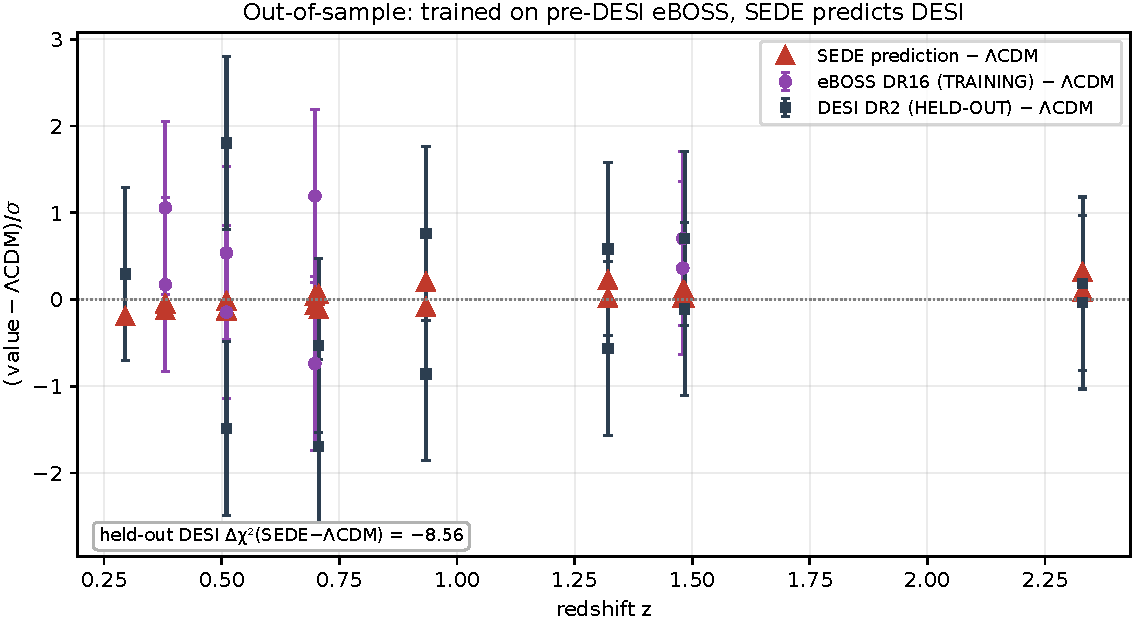
\includegraphics[keepaspectratio]{../../results/paper/fig5_oos}}
\caption{Out-of-sample test. BAO residuals relative to
\(\Lambda \mathrm{CDM}\) (in \(\sigma\)) for the training set (pre-DESI
eBOSS DR16, purple) and the held-out DESI DR2 data (slate), with the
SEDE prediction (red) from parameters fit to eBOSS alone. SEDE, trained
without ever seeing DESI, predicts the held-out DESI BAO better than
\(\Lambda \mathrm{CDM}\) \((\Delta \chi ^{2} = -8.56)\) in this split
--- encouraging, and to be independently reproduced.}\label{fig:7}
\end{figure}

\subsection{Robustness}\label{sec-5-4}

The preference is not a single-dataset artifact. (i)
\textbf{Supernova-set independence:}
\(\Delta \chi ^{2}(\mathrm{SEDE} - \Lambda \mathrm{CDM})\) is
\(\approx  -4.7\) with Pantheon+ and, because the SN channel contributes
only +0.17 to the total, is SN-set-independent (DES-5YR/Union3 shift it
by \(\lesssim 0.1\)) --- not a Pantheon+ effect. (ii) Per-probe
decomposition (where the preference comes from). Decomposing the joint
\(\Delta \chi ^{2}(\mathrm{SEDE} - \Lambda \mathrm{CDM}) = -4.68\) into
per-probe contributions \emph{at the joint best-fit} is more informative
than the leave-one-out, and we report it plainly: the preference is
carried by the geometry channels --- the compressed CMB distance (R,
ℓ\_A) contributes \(-2.80\) and the SH0ES \(H_{0}\) prior \(-1.78\)
\((together \approx  98\)\% of the total) --- while DESI BAO
\((-0.29)\), \(f\sigma 8\) \((-0.03)\) and \(\omega _{\mathrm{b}}\)
\((-0.05)\) are nearly flat and Pantheon+ SN (+0.17) and cosmic
chronometers (+0.10) marginally favour \(\Lambda \mathrm{CDM}\). So this
is \textbf{not a broad multi-probe consensus}: SEDE's evolving w(z) fits
the distance to last scattering better and accommodates a marginally
higher \(H_{0}\) (68.9 vs 68.7) that eases SH0ES --- a \emph{paired}
(CMB-distance \(+ H_{0}\)) effect. We show the decomposition precisely
because the leave-one-probe-out is blind to this paired structure
(dropping either member leaves the other, so every single-probe holdout
stays negative: shallowest \(\approx  -1.9\) when the CMB-distance is
the dropped probe, deepest \(\approx  -4.85\)) --- the holdout
robustness is real but does not by itself establish a consensus. Two
qualifications follow. First, the CMB-distance contribution is
\emph{not} a compressed-prior artifact: folding the full primary CMB
into the joint keeps it \((\Delta \chi ^{2} = -3.17\), §\ref{sec-5-1};
§\ref{sec-4-2} red-team). Second, SEDE does not resolve the Hubble
tension --- its best-fit \(H_{0} \approx  69\) still sits ∼\(4\sigma\)
from SH0ES (§\ref{sec-7}, §\ref{sec-9}) --- but its geometry does ease
the SH0ES prior by \(\Delta \chi ^{2} \approx  1.8\), so part of the
preference is a mild \(H_{0}\) accommodation, which we flag rather than
hide. (ii′) No-SH0ES robustness (the contested prior removed). Because
the SH0ES \(H_{0}\) prior is the field's most disputed input --- and
DESI's own baseline excludes it --- we recompute all three headline
statistics with SH0ES dropped. The preference weakens but survives, and
what remains sits in the harder channel. The joint
\(\Delta \chi ^{2}(\mathrm{SEDE} - \Lambda \mathrm{CDM}) = -2.89\)
\((from -4.68)\), now carried by the compressed CMB distance and DESI
BAO, with the best-fit \(H_{0}\) falling to 68.4 once it is no longer
pulled toward 73 --- i.e.~the CMB-distance improvement is genuine, not
an \(H_{0}\) accommodation. The Bayesian evidence falls to ln
\(B \approx  +1.4\) (Laplace; still \emph{positive}, moderate-to-weak)
--- and the false-preference calibration (§\ref{sec-5-2}) weakens to
∼\(2.3\sigma\) versus ∼\(3\sigma\) with SH0ES. So roughly 38\% of the
\(\chi ^{2}\) preference is carried by SH0ES; the remainder is robust
and lives in the CMB-distance channel rather than the contested local
prior. We read this as sharpening, not weakening, the paper's
``moderate, not established'' posture: with the one disputed prior
removed, SEDE remains preferred (∼\(2.3\sigma\)) by hard geometric data,
and no part of that residual depends on resolving the Hubble tension.
(iii) \textbf{Code independence:} the SEDE expansion history reproduced
with CLASS matches CAMB to \(5\times 10^{-5}\) in \(r_{\mathrm{drag}}\)
\((\)≪ 0.2\%) --- not a CAMB artifact. (iv) \textbf{Growth:} the
full-Boltzmann \(\gamma _{\mathrm{growth}} \approx  0.55\)
\citep{Linder:2007hg} confirms standard-GR dark energy at the background
level; the completed FPAB perturbations do carry a mild sub-horizon
enhancement \((\mu _\infty  \approx  1.05\) in the \(\mu\)--\(\Sigma\)
language \citep{Pogosian:2016pwr, Silvestri:2013ne}) that \emph{raises}
growth --- opposite to the mild suppression \((\gamma  > 0.55)\) current
data prefer \citep{Nguyen:2023fip}, a genuine falsifiable risk rather
than an S8-easing accommodation. (v) \textbf{Tracer-level robustness:}
recent analyses argue the DESI DR2 evolving-DE signal is driven mainly
by the LRG1 \((z\approx 0.51)\) and LRG2 \((z\approx 0.71)\) BAO bins
\citep{Chaudhary:2025vzy, Wang:2025bkk}. Dropping these bins
individually and together leaves SEDE's preference intact ---
\(\Delta \chi ^{2}(\mathrm{SEDE} - \Lambda \mathrm{CDM}) = -5.07\)
\((-\mathrm{LRG}1)\), −4.28 \((-\mathrm{LRG}2)\), and \(-4.57\) with
both removed \((versus -4.68\) for the full set), negative in every
tracer holdout (range \([-5.07\), −4.28{]}). SEDE's preference is
therefore \emph{not} the LRG1--2 artefact the steep-CPL signal is
attributed to: it is a geometry-channel preference (CMB-distance
\(+ H_{0}\), §\ref{sec-5-4}(ii)) that does not rest on the contested
bins. The dissociation is quantitative: the
\(\Lambda \mathrm{CDM}\)-deviation measured by the
\(ratio(\omega _{\mathrm{m}})\) early-vs-late consistency metric drops
from \(2.6\sigma\) to \(1.2\sigma\) when LRG1--2 are removed
\citep{Liu:2024gfy}, whereas SEDE's \(\Delta \chi ^{2}\) is essentially
unchanged \((-4.68\) → −4.57) --- SEDE's preference and the LRG-driven
steep-CPL deviation are \emph{different objects}. This is the natural
answer to the post-DR2 robustness critiques (§\ref{sec-5-7}). (vi) The
fixed structure coupling \(\gamma\) (systematic robustness). The
headline is computed at the halo-statistics value \(\gamma  = 1.50\),
but §\ref{sec-3-1} assigns \(\gamma\) a mass-function/mass-range
systematic \(\gamma  \in  [1.14\), 1.60{]}. Propagating that band
through profiled re-fits at fixed \(\gamma  = 1.14\), 1.30, 1.50, 1.60
leaves the preference intact throughout:
\(\Delta \chi ^{2} \in  [-2.1\), −4.7{]}
\((\gamma  = 1.14/1.30/1.50/1.60\) → −\(2.1/-4.4/-4.7/-3.8\)),
Barrow-preferred at every \(\gamma\), weakening to \(\approx  -2.1\) at
the low-\(\gamma\) endpoint without inverting and peaking near the
theory value. So the preference is not an artifact of the specific
\(\gamma\); and --- a mild consistency point --- the data prefer
\(\gamma\) close to the binding-energy-derived value (§\ref{sec-3-1})
rather than the band edges. (One caveat for the equation of state, not
the fit: at \(\gamma  \lesssim  1.45\) the background is phantom-today,
\(w_{0} < -1\), so the DESI-quadrant \(w = -1\) crossing of
§\ref{sec-3-2} is a property of the upper half of the \(\gamma\) band;
the \emph{fit} preference holds across the whole band.)

\subsection{Evidential summary}\label{sec-5-5}

SEDE is moderately preferred over \(\Lambda \mathrm{CDM}\)
\((\Delta \mathrm{DIC} \approx  -3.5\) to \(-4.7\); calibration p
\textless{} 0.0015, 0/2000, ∼2--\(3\sigma\) across pipelines,
∼\(2.3\sigma\) without SH0ES); the preference is not obviously
attributable to model flexibility, and is supported by a pre-DESI → DESI
out-of-sample check --- and the model adds no continuously-sampled
dark-energy parameter. It is not decisive: both models fit the
compilation well \((\chi ^{2}/dof \approx  0.88)\), so this is a
\emph{relative} preference on a single compiled dataset, stronger than
indistinguishable but short of established. DESI DR3 and Euclid provide
the sharp future test (§\ref{sec-6}).

\textbf{What the preference is against --- and what it is not.} The
headline figure is deliberately the SH0ES-free ∼\(2.3\sigma\): with
SH0ES included it reaches ∼2--\(3\sigma\), but the SH0ES-free value is
the one not inflated by the Planck--SH0ES \(H_{0}\) tension. The
preference is corroborated across criteria that do not share DIC's
point-estimate sensitivity --- \(\Delta \chi ^{2} = -4.68\)
(frequentist), a Laplace ln B (Occam-neutral because \(\Delta k = 0\)),
and \(\Delta \mathrm{AIC} = \Delta \mathrm{BIC} = \Delta \chi ^{2}\)
(equal parameter count) --- and the three supernova compilations enter
as \emph{alternatives} (Pantheon+ baseline; DES-5YR and Union3 as
independent robustness swaps, §\ref{sec-5-4}), never stacked, so no
shared low-z anchor is multiply counted. Crucially, this is \emph{not}
the DESI evolving-dark-energy signal re-badged: SEDE's \((w_{0}\),
\(w_{\mathrm{a}}\)) sits ∼\(2.7\sigma\) from the DESI DR2 preferred
point (and only ∼\(0.5\sigma\) from \(\Lambda \mathrm{CDM}\),
§\ref{sec-5-1}), and the preference \emph{survives dropping the LRG1--2
bins} that drive the DESI steep-\(w_{\mathrm{a}}\) signal (tracer-level
leave-one-out, §\ref{sec-5-4}: \(\Delta \chi ^{2} = -5.07 / -4.28\) with
LRG1 / LRG2 removed) --- a preference that persists after deleting the
signal's putative source is a distinct object. The background w(z) is
itself CPL-degenerate in shape
(max\textbar{}\(w - w_\mathrm{CPL}\)\textbar{} = 0.027, §\ref{sec-5-6}),
so what separates SEDE from a generic \(w_{0}w_{\mathrm{a}}\) fit is not
the expansion history but (i) \emph{parsimony} --- SEDE reaches the same
w(z) with zero extra parameters against
\(w_{0}w_{\mathrm{a}}\mathrm{CDM}'s\) two, so at comparable fit it is
favoured on Bayesian evidence --- and (ii) the growth, ISW, and
\(\Delta\) channels a CPL doppelgänger cannot reproduce (§\ref{sec-6}).
A direct DIC comparison on this likelihood bears this out: SEDE and
\(w_{0}w_{\mathrm{a}}\mathrm{CDM}\) fit \emph{comparably} in
\(\chi ^{2}\), with SEDE favoured by its ∼2 fewer effective parameters
\((p_{\mathrm{D}} \approx  5\) versus \(\approx  7\)); and marginalising
SEDE's shape parameters \(\gamma\) and \(\Delta\) leaves the
\(\Lambda \mathrm{CDM}\) preference \emph{essentially unchanged}
(hidden-parameter penalty \(\lesssim  0.2\) in DIC) --- so the
preference is neither the generic evolving-DE signal nor an artifact of
holding the shape fixed. The full model set \((\Lambda \mathrm{CDM}\),
SEDE, \(w_{0}w_{\mathrm{a}}\mathrm{CDM}\), and free-shape SEDE) and a
Bayesian-evidence cross-check are carried out by
\texttt{run\_model\_comparison.py} in the reproduction repository.

\subsection{\texorpdfstring{The deformation \(\Delta\) from current data
--- a conditional
diagnostic}{The deformation \textbackslash Delta from current data --- a conditional diagnostic}}\label{sec-5-6}

The Barrow parameter \(\Delta\) is a useful \emph{test} axis: the volume
postulate corresponds to \(\Delta  = 1\), the area law to
\(\Delta  = 0\). SEDE's \emph{equation of state} is CPL-degenerate in
shape (max\textbar{}\(w - w_\mathrm{CPL}\)\textbar{} = 0.027), so a
diagnostic must use channels other than the EOS curvature. We stress at
the outset that the numbers below are conditional diagnostics (computed
with the other cosmological and nuisance parameters held at or near
their best-fit values, not a full marginalised likelihood with
\(\Delta\) varied); they indicate where current data sit, not a
marginalised detection. Four channels:

\begin{longtable}[]{@{}
  >{\raggedright\arraybackslash}p{(\linewidth - 4\tabcolsep) * \real{0.3333}}
  >{\raggedright\arraybackslash}p{(\linewidth - 4\tabcolsep) * \real{0.3333}}
  >{\raggedright\arraybackslash}p{(\linewidth - 4\tabcolsep) * \real{0.3333}}@{}}
\toprule\noalign{}
\begin{minipage}[b]{\linewidth}\raggedright
channel
\end{minipage} & \begin{minipage}[b]{\linewidth}\raggedright
what it uses
\end{minipage} & \begin{minipage}[b]{\linewidth}\raggedright
\(\hat{\Delta}\) (conditional profile --- not a posterior)
\end{minipage} \\
\midrule\noalign{}
\endhead
\bottomrule\noalign{}
\endlastfoot
CMB shift parameter R (Planck) & early-DE fraction,
\(\Omega _\mathrm{DE}(z_{\mathrm{rec}}) \propto  H^{-\Delta }\) & 0.98 ±
0.11 \\
lever arm: DESI \(\mathrm{BAO} + Ly\alpha (z=2.33) + R\) &
\(\rho _\mathrm{DE}/\rho _{\mathrm{crit}} \propto  H^{-\Delta }\) across
the H-range & 1.03 ± 0.11 \\
DESI DR2 \((w_{0}\),\(w_{\mathrm{a}}\)) quadrant (official chains) & EOS
values + crossing & 0.93 / 0.83 / 0.90 (PantheonPlus/DESY5/Union3) \\
growth \(f\sigma 8\) \citep{Sagredo:2018ahx} --- orthogonal & growth
amplitude, not distance & 0.0 ± 0.61 \\
\end{longtable}

\begin{quote}
These are not posterior constraints on \(\Delta\); they are
profile/conditional diagnostics --- each \(\hat{\Delta}\) is obtained
with the other cosmological and nuisance parameters held at (or near)
their best-fit values, \emph{not} marginalised. The quoted ± is the
conditional curvature width, not a marginalised error bar; read each row
as ``the data lean to \(\Delta  \approx  1\) in this channel,'' not as a
measurement. The robust, marginalised \(\Delta\) measurement awaits DESI
DR3 + Euclid (§\ref{sec-6}).
\end{quote}

These diagnostics prefer the volume endpoint \((\Delta  \approx  1)\)
and disfavour the area-law branch \((\Delta  = 0)\), consistent with the
EOS argument of §\ref{sec-8-1} (the area-law branch has
\(w_{0} = -0.49\) and an outsized early-DE fraction). The growth channel
is weak but orthogonal (growth amplitude, not expansion) and is
consistent with the geometric value at \(1.6\sigma\) --- no
growth--geometry tension.

The high apparent significance of the area-law disfavouring is a
conditional statement and must not be read as a marginalised detection:
the CMB and lever-arm channels share the high-z expansion, so their
combination is an upper bound on the information, and it is conditional
on \(\Omega _{\mathrm{m}}\), \(H_{0}\), \(r_{\mathrm{d}}\) ---
marginalising, the area-law signal is partly reabsorbed by shifts in
those parameters. This is exactly why the \emph{joint, marginalised}
model preference is moderate \((\Delta \mathrm{DIC} \approx  -4.7\),
§\ref{sec-5-1}--§\ref{sec-5-5}), not overwhelming; the two statements
are not in tension once the conditional-vs-marginal distinction is kept.
The \((w_{0}\),\(w_{\mathrm{a}}\)) channel also pulls slightly low
because SEDE's gentle \(w_{\mathrm{a}}\) under-matches DESI's steeper
preferred \(w_{\mathrm{a}}\) --- the same mild ∼\(2.7\sigma\) EOS
tension visible in the joint fit (Fig. 4). In summary: current late-time
data prefer the volume endpoint and disfavour the area-law branch, but a
robust \emph{marginalised} measurement of \(\Delta\) awaits DESI DR3 and
Euclid (§\ref{sec-6}). The foundations companion paper (§\ref{sec-7})
\citep{Pandev:2026foundations} sharpens the present-data statement one
step beyond these conditional channels with a \emph{profile-likelihood}
interval for the gated family --- all base parameters re-optimised at
each \(\Delta\) --- giving \(\Delta  = 0.93\) {[}0.83, 1.02{]}, with
\(\Delta  = 0\) excluded at \(\Delta \chi ^{2} \approx  371\). This is
stronger than the conditional diagnostics tabulated here, but it is
still a profile, not the full marginalised posterior, which remains the
DR3 + Euclid target --- and, read as a profile, it overstates the
marginalised model-level signal (the
\(\Delta \mathrm{DIC} \approx  -4.7\) of §\ref{sec-5-1}--§\ref{sec-5-5})
by roughly two orders of magnitude in \(\chi ^{2}\), so it must not be
quoted as a posterior exclusion of the area law.

\subsection{Relation to the post-DESI DR2 literature}\label{sec-5-7}

The DESI DR2 BAO release \citep{DESI:2025zgx} sharpened interest in
evolving dark energy, with a preference for the \((w_{0} > -1\),
\(w_{\mathrm{a}} < 0\)) quadrant; the subsequent literature is actively
debating whether that signal is physical or an artefact of dataset
combination, tracer selection, or supernova calibration
\citep{Turyshev:2026ewm}. Two threads bear directly on SEDE. First,
robustness critiques argue the steep signal reflects CMB/BAO/SN
combination tension \citep{Wang:2025bkk} and is driven mainly by the
LRG1--2 BAO bins \citep{Chaudhary:2025vzy, Liu:2024gfy}. This
\emph{helps} SEDE rather than threatening it: SEDE does not chase the
steep \(w_{\mathrm{a}}\) (it sits ∼\(2.7\sigma\) from the DESI CPL
point, §\ref{sec-5-6}), and its preference survives a tracer-level
leave-one-out that removes exactly those LRG1--2 bins (§\ref{sec-5-4},
\(\Delta \chi ^{2} = -4.57\) with both dropped) --- so SEDE realises the
\emph{conservative} reading the critiques call for, rather than the
fragile steep-CPL one. Second, \textbf{reconstruction and mechanism
papers}: model-agnostic Gaussian-process reconstructions place the
\(w = -1\) crossing at \(z_{\mathrm{wt}} \approx  0.46\)
\((+0.24/-0.12)\) \citep{Zhang:2025bmk}, versus SEDE's canonical
\(z \approx  0.19\) --- a ∼\(2.2\sigma\) offset (SEDE crosses more
recently) that is a genuine future discriminator, not yet a tension
given the broad reconstruction errors. Among mechanism competitors,
data-driven analyses read the evolving signal as a \emph{coupled} dark
sector (∼\(2.2\sigma\) DE--DM interaction at low z) \citep{You:2025uon};
SEDE's CHR ledger is exactly such a coupling but with the interaction
\emph{fixed} to the structure-growth rate, \(c_{\mathrm{s}}^{2} = 1\),
and instability-free (§\ref{sec-7}), rather than a free coupling. And
the quintom programme \citep{Cai:2025mas, Thanankullaphong:2026anl}
rests on a \emph{no-go theorem} --- no single canonical field or perfect
fluid crosses \(w = -1\), so viable models require two fields, higher
derivatives, modified gravity, or an effective-field-theory description.
SEDE is the last of these: it crosses \(w = -1\) \emph{effectively}, as
a smooth horizon fluid in the GW-safe EFT corner
\((\alpha _{\mathrm{T}} = \alpha _{\mathrm{M}} = 0\),
\(c_{\mathrm{s}}^{2} = 1\); §\ref{sec-7}), avoiding the ghost/two-field
machinery, and --- unlike the two-field quintom whose late attractor is
phantom-dominated (a Big-Rip tendency) \citep{Thanankullaphong:2026anl}
--- SEDE's future attractor is de Sitter (w → −1, with
\(f_{\mathrm{sat}}\) \emph{saturating} to a finite \(\approx 1.23\) as
growth freezes, not diverging; §\ref{sec-2}, Appendix~\ref{sec-A}.7,
Result 12), so it does not predict a Big Rip.

Two further consistency points sharpen the post-DR2 placement. (a)
\textbf{Turyshev's model filter.} The DR2 status review
\citep{Turyshev:2026ewm} screens evolving-DE models by
\emph{gravitational-wave propagation} and \emph{perturbation stability},
and stresses that the CPL preference is sensitive to redshift-dependent
SN calibration at the \(few\times 10^{-2}\) mag level. SEDE passes the
filter by construction \((\alpha _{\mathrm{T}} = 0\) ⟹
\(c_\mathrm{GW} = c\); \(c_{\mathrm{s}}^{2} = 1\) ⟹
gradient/ghost-stable; §\ref{sec-7}), and its SN-set independence (the
SN channel contributes only +0.17, so the \(\approx  -4.7\) preference
is SN-set-independent; §\ref{sec-5-4}) limits the calibration exposure.
(b) The \(r_{\mathrm{d}}\)-independent shape test. Turyshev's
calibration-free observable
\(F_\mathrm{AP}(z) \equiv  D_{\mathrm{M}}/D_{\mathrm{H}} = (D_{\mathrm{M}}/r_{\mathrm{d}})/(D_{\mathrm{H}}/r_{\mathrm{d}})\)
cancels the sound horizon and is also \(H_{0}\)-independent, isolating
the pure expansion shape E(z). On the six DESI DR2 tracer bins that
report both ratios, SEDE's evolving-w shape gives \(\chi ^{2}/n = 0.96\)
--- consistent with the data and indistinguishable from
\(\Lambda \mathrm{CDM}\) \((\Delta \chi ^{2} = -0.14)\) --- with no
reliance on \(r_{\mathrm{d}}\), \(H_{0}\), the CMB sound horizon, or SN
calibration, the very systematics the robustness debate targets. (The
LRG1 bin sits ∼\(1.8\sigma\) low for \emph{both} SEDE and
\(\Lambda \mathrm{CDM}\), i.e.~it is a data feature, not a model
failure.) SEDE is thus a \emph{physical} member of the post-DR2
evolving-DE family, distinguished by its mechanism (the
growth--expansion lock, §\ref{sec-6}), by passing the stability/GW
filter, and by surviving the robustness and calibration-free tests the
steep signal may not.

\section{Predictions and falsifiability}\label{sec-6}

Because SEDE adds no fitted dark-energy parameter, it makes sharp
predictions rather than fits. We pre-registered these (a sha256-locked
statement deposited ahead of the future data; Appendix~\ref{sec-D}) to
forbid post-hoc tuning:

\begin{longtable}[]{@{}
  >{\raggedright\arraybackslash}p{(\linewidth - 4\tabcolsep) * \real{0.3333}}
  >{\raggedright\arraybackslash}p{(\linewidth - 4\tabcolsep) * \real{0.3333}}
  >{\raggedright\arraybackslash}p{(\linewidth - 4\tabcolsep) * \real{0.3333}}@{}}
\toprule\noalign{}
\begin{minipage}[b]{\linewidth}\raggedright
quantity
\end{minipage} & \begin{minipage}[b]{\linewidth}\raggedright
SEDE prediction
\end{minipage} & \begin{minipage}[b]{\linewidth}\raggedright
discriminating from
\end{minipage} \\
\midrule\noalign{}
\endhead
\bottomrule\noalign{}
\endlastfoot
Barrow deformation \(\Delta\) & 1.0 ± 0.09 (forecast) & a smooth horizon
\(\Delta  = 0\) \\
equation of state \((w_{0}\), \(w_{\mathrm{a}}\)) & ≈ \((-0.98\),
−0.11), crossing \(-1\) & the DESI DR2 preferred point at ∼\(2.7\sigma\)
(only ∼\(0.5\sigma\) from \(\Lambda \mathrm{CDM}\) --- the EOS is
\emph{not} a \(\Lambda \mathrm{CDM}\) discriminator; \(\Delta\) is) \\
\(w = -1\) crossing redshift (consistency check, \emph{not} a
discriminator) & \(z \approx  0.19\) (GH-convention volume-law value,
convention-conditional; ∼\(2.2\sigma\) mild tension) & GP
reconstructions \(z_{\mathrm{wt}} \approx  0.46\) \((+0.24/-0.12)\)
\citep{Zhang:2025bmk} \\
structure amplitude \(\sigma 8\) & ≈ 0.811 (FPAB-SEDE; \emph{raises}
growth vs \(\Lambda \mathrm{CDM}\) 0.800) & a smooth-fluid
\(c_{\mathrm{s}}^{2}=1\) \(\sigma 8 \approx  0.76\) (retracted) \\
gravitational slip / force & \(\gamma_{\rm slip}\) = 1;
\(\mu_\infty(0)\) = 1.05, turn-on \(k_{50}\)--\(k_{90}\) = (0.70--2.1)
aH & \(\Lambda \mathrm{CDM}\) \((\mu  = 1\), no scale-dependent
force) \\
growth index \(\gamma _{\mathrm{growth}}\) & ≈ 0.55 & modified gravity
\((\gamma _{\mathrm{growth}} \neq  0.55)\) \\
\end{longtable}

\sloppy

The growth-side rows \((\sigma 8\), gravitational slip/force) are
\emph{conditional on the FPAB-SEDE completion}, which is
trajectory-level (one calibrated cubic-KGB member reproducing the
background, not a theorem that every solution is healthy; §\ref{sec-7})
and awaits a full perturbative refit (§\ref{sec-4-4}) --- they are
forecasts, not yet marginalised measurements. The full machine-readable
prediction set is committed as \texttt{predictions.json} in the
reproduction repository, cryptographically locked by
\texttt{sha256(predictions.json)} =
\texttt{4e2ca4b5\allowbreak{}721ef60a\allowbreak{}68a7e78e\allowbreak{}033f0a1d\allowbreak{}5f565f82\allowbreak{}7656ee4d\allowbreak{}49901d5c\allowbreak{}58d059ce};
it is regenerated byte-for-byte by \texttt{gen\_predictions.py}, so the
registered values cannot be altered after this digest is published.

\fussy

A near-term tension --- and what \(z \approx  0.19\) is and is not.
Canonical SEDE crosses \(w = -1\) at \(z_{\mathrm{cross}} = 0.195\)
\((w_{0} = -0.996)\), using the Gibbons--Hawking horizon temperature
\(T_\mathrm{AH} = H/2\pi\). We state the status of this number honestly:
it is \emph{convention-conditional}, not a convention-free prediction.
\(T = H/2\pi\) is the de Sitter temperature appropriate for a de
Sitter-attractor dark-energy fluid, and we \emph{tested} the alternative
--- applying the full dynamical Cai--Kim factor \((1-\epsilon /2)\) to
the volume-law fluid (the self-consistent
\(\rho _\mathrm{DE} \propto  H(1-\epsilon /2)f\) model). It
\textbf{fails}: it has no stable self-consistent background, and in the
stable perturbative limit it gives \(w_{0} = -1.15\) and stays phantom
\((w < -1)\) at all z --- no crossing at all, and in the \emph{wrong}
DESI quadrant \((w_{0} < -1)\). That failure motivates the
Gibbons--Hawking choice, but it also means the surviving convention is
\emph{selected} in part because it yields a crossing in the viable
quadrant: \(z \approx  0.19\) is the crossing of the GH-convention
volume-law model, an output of the adopted temperature convention rather
than a knob --- but not a prediction independent of that convention.
(The unrelated \(z \approx  0.59\) is the \emph{area-law}
\(\Delta  = 0\) model ---
\(\rho _\mathrm{DE} \propto  H^{2}(1-\epsilon /2)f\) --- a different
model, not a convention of this one.) Post-DR2 Gaussian-process
reconstructions favour \(z_{\mathrm{wt}} \approx  0.46\)
\((+0.24/-0.12)\) \citep{Zhang:2025bmk, You:2025uon}; canonical SEDE
sits ∼\(2.2\sigma\) more recent --- a \emph{real, mild} tension (the
reconstruction's lower error is tight), the one place current data pull
against canonical SEDE. We flag it as such, not as a discriminator: the
crossing redshift is CPL-degenerate (§\ref{sec-6}, below) and, read as a
\(\Delta\)-probe, would point the \emph{wrong} way (toward
\(\Delta  = 0\)), conflicting with the early-DE diagnostics that favour
\(\Delta  = 1\) (§\ref{sec-5-6}). The model's actual test is the
deformation amplitude \(\Delta\), not the crossing; a DR3/Euclid
measurement of the crossing is a useful consistency check, not the
decider.

\textbf{The sharp future test.} The discriminating observable is the
\emph{amplitude} of the deformation \(\Delta\), not the detailed shape
of w(z) --- indeed the SEDE w(z) is CPL-degenerate in shape to better
than the DR3 precision (max \textbar{}\(w - \mathrm{CPL}\)\textbar{} ≈
0.027), so a CPL fit cannot distinguish the \emph{mechanism}; \(\Delta\)
can. A Fisher forecast in \((\Omega _{\mathrm{m}}\), \(\Delta\), ln A
\(r_{\mathrm{d}}\)) gives \(\sigma (\Delta ) \approx  0.115\) from DESI
DR3 alone, 0.133 from Euclid, and \(\sigma (\Delta ) \approx  0.087\)
combined --- a nominal ∼\(11\sigma\) separation of the volume-law
horizon \((\Delta  = 1)\) from a smooth one \((\Delta  = 0)\). This
``∼\(11\sigma\)'' is a \emph{conditional, pre-marginalisation} Fisher
number and must be read against §\ref{sec-5-6}: \(\Delta\) is strongly
degenerate with \((\Omega _{\mathrm{m}}\), \(H_{0}\),
\(r_{\mathrm{d}}\)), and the present-data conditional channels give
\(\sigma (\Delta ) \approx  0.11\) while the \emph{marginalised} model
preference is only \(\Delta \mathrm{DIC} \approx  -4.7\) --- a roughly
two-orders-of-magnitude conditional→marginalised degradation the same
Fisher forecast (a fixed-fiducial, Gaussian object) will suffer. So the
realistic marginalised separation is expected to be \emph{well below}
\(11\sigma\), and the honest framing --- used everywhere else --- is
that \(\Delta\) is a discrete \emph{model-selection} target
\((\Delta  = 1\) vs \(\Delta  = 0\)) for DESI DR3 + Euclid, not an
\(11\sigma\) measurement.

The mechanism test is also forecast to be decisive --- separately from
the amplitude. The \(\sigma (\Delta )\) above is the
\emph{geometry-side} deformation; the \emph{distinctive} SEDE claim
(dark energy sourced by structure) is tested by measuring \(\Delta\) on
the growth side and checking it against the geometry side --- the E1/P2
growth--expansion lock. A Fisher forecast for the growth-side
deformation gives \(\sigma (\Delta )_{\mathrm{growth}} = 0.25\) from
Euclid/LSST weak lensing alone, tightening to 0.13 (∼\(4\sigma\)) when
combined with CMB-lensing, cluster abundance, RSD, and kSZ. Reframed as
the parameter-free null test
\(r(z) \equiv  \rho _\mathrm{DE}^{geom}(z) - G[D^{growth}(z)] = 0\) ---
dark energy a fixed function of the linear growth factor --- the test
uses the full redshift shape with no dark-energy parameters;
\(\Lambda \mathrm{CDM}\) \((\rho _\mathrm{DE} = const\), no
D-dependence) and Gough's information-DE
\((\rho _\mathrm{DE} = G\)′{[}SMD{]}, baryonic) violate it distinctly.
So Euclid/LSST-era growth data are forecast to confirm or refute the
structure-sourcing mechanism at ∼\(4\sigma\), not merely the EOS shape
--- closing the gap between ``a w(z) with a thermodynamic story'' and a
tested mechanism (§\ref{sec-9}). The exact data vector (the geometry leg
DESI DR3 \(D_{\mathrm{H}}/r_{\mathrm{d}}\)→H(z) vs the growth leg
Euclid/LSST \(3\times 2pt + \mathrm{CMB}\)-lensing + clusters + RSD) and
the pre-registered decision rule --- CONFIRM if
\textbar{}\(\Delta _{\mathrm{grow}} - \Delta _{\mathrm{geom}}\)\textbar{}
\textless{} \(2\sigma\) with the null
\(r(z) = \rho _\mathrm{DE}^{geom} - G[D^{grow}] = 0\) at
\(\chi ^{2}/dof \lesssim  1\); REFUTE if \(\Delta _{\mathrm{grow}}\) is
consistent with 0 at \(>3\sigma\) while \(\Delta _{\mathrm{geom}} = 1\)
--- are locked in the pre-registration (§\ref{sec-F};
Appendix~\ref{sec-D}), so the staged test carries no post-hoc freedom.

\begin{figure}
\centering
\pandocbounded{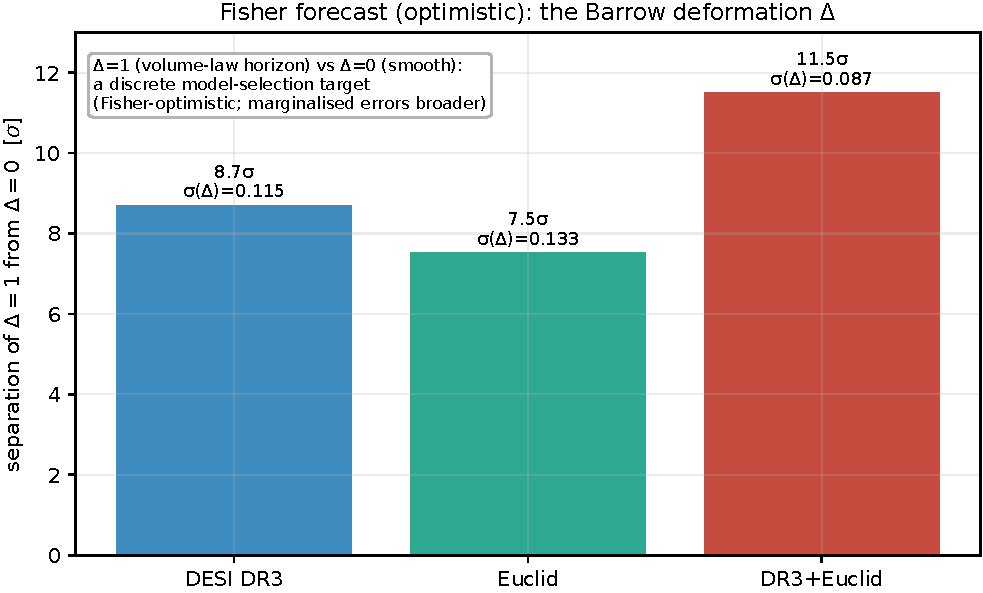
\includegraphics[keepaspectratio]{../../results/paper/fig6_forecast}}
\caption{The sharp future test. A Fisher forecast (optimistic by
construction) of the separation of the volume-law horizon
\((\Delta = 1)\) from a smooth one \((\Delta = 0)\): DESI DR3 reaches
\(8.7\sigma\), Euclid \(7.5\sigma\), and the combination
\(\sigma (\Delta ) \approx 0.087\), a nominal ∼\(11\sigma\) separation.
The moderate present preference would become a strong test with the next
generation of surveys.}\label{fig:8}
\end{figure}

\begin{figure}
\centering
\pandocbounded{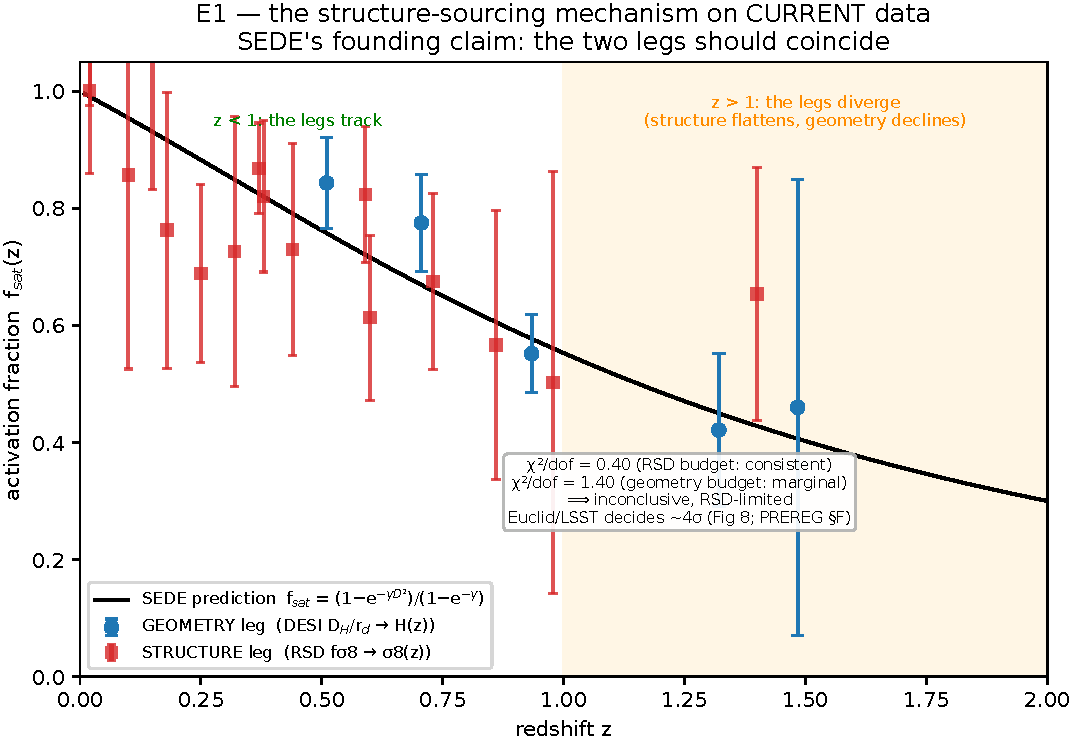
\includegraphics[keepaspectratio]{../../results/fig_e1_mechanism}}
\caption{The structure-sourcing mechanism on \emph{current} data (the
companion to the forecast of Figure 8, and the paper's open frontier).
SEDE's founding claim is that the activation fraction
\(f_{\mathrm{sat}}\) read off the expansion (geometry leg: DESI
\(D_{\mathrm{H}}/r_{\mathrm{d}}\) → H(z), blue) coincides with the one
read off structure growth (RSD \(f\sigma 8\) → \(\sigma 8(z)\) → D(z),
red); the black curve is the SEDE prediction both should follow. The two
legs track at z \textless{} 1 but diverge at z \textgreater{} 1 (the
structure leg flattens while the geometry/model declines). The
significance is error-budget-dependent --- \(\chi ^{2}/dof = 0.40\) in
the RSD-error budget (consistent) versus 1.40 in the precise-geometry
budget (marginally disfavoured \emph{in that budget} --- though
§\ref{sec-9} shows this offset is the shared \(\Lambda \mathrm{CDM}\) S8
tension {[}\citep{Pantos:2026koc}{]}, not a SEDE-specific failure) ---
so on present data the mechanism is \textbf{inconclusive and
RSD-limited}: SEDE's EOS is favoured, but its distinctive mechanism is
not yet confirmed. Euclid/LSST weak-lensing tomography and the Euclid
spectroscopic growth measurement {[}\citep{Majerotto:2012mf}{]} sharpen
the structure leg and decide this at ∼\(4\sigma\) (Figure 8;
pre-registered decision rule, pre-registration
§\ref{sec-F}).}\label{fig:9}
\end{figure}

A near-term consistency probe: the \(\mathrm{ISW}\times galaxy\)
cross-correlation \citep{Afshordi:2004kz}. The smooth-fluid closure
\((c_{\mathrm{s}}^{2} = 1\), §\ref{sec-3-4}) refers to the
\emph{sub-horizon} response; on the largest scales the structure gate
carries a coupling of the dark-energy perturbation to matter,
\(\beta  \equiv  d\) ln \(f_{\mathrm{sat}}/d\) ln
\(D \approx  0.9\)--1.5, that is \emph{not} (1+w)-suppressed. That an
O(1) dark-sector coupling escapes the (1+w) suppression of clustering
quintessence and enhances the low-ℓ integrated Sachs--Wolfe signal is a
known feature of coupled dark energy
\citep{Schafer:2008uc, Mainini:2007ft, Hu:2004yd}; what is specific to
SEDE is that the coupling is \emph{fixed} by the growth gate, giving a
definite, horizon-scale \((\ell  \lesssim  10)\)
\(\mathrm{ISW}\times galaxy\) excess over
\(\Lambda \mathrm{CDM}/\mathrm{CPL}\) --- a forecast-grade few-percent
effect (a matched-cosmology estimate gives \(\approx  +13\)\% at ℓ = 2,
≈ +4\% averaged over ℓ ≤ 10). Unlike the \(f\sigma 8\) growth-lock,
which is CPL-degenerate and carries no detectable signal, this excess
does \emph{not} cancel against a CPL doppelgänger. It is testable now
(Planck ISW × DES/unWISE), cosmic-variance-limited, and cuts both ways:
a \emph{large} small-scale signal is already excluded. The low-ℓ
temperature-side signature is no longer only an estimate: the FPAB-SEDE
spectrum, computed through the full modified-gravity Boltzmann code,
gives a stable, converged low-ℓ ISW suppression ---
\(C_\ell ^\mathrm{TT}(\mathrm{SEDE})/C_\ell ^\mathrm{TT}(\Lambda \mathrm{CDM}) = 0.924\)
at ℓ = 2 \((-7.6\)\%), within 0.5\% of unity by ℓ ≈ 50 and recovering
unity by ℓ ≈ 100, with the primary acoustic peaks unchanged (ratio
0.9999 at ℓ = 220) --- verified to be independent of the numerical
GR-transition redshift of the solver (the observational-tests companion
paper). (The two ℓ = 2 numbers above are different observables and
consistently signed: the enhanced late-time ISW source \emph{raises} the
\(\mathrm{ISW}\times galaxy\) cross-spectrum, +13\%, while
\emph{suppressing} the temperature auto-spectrum, −7.6\% --- the
standard auto-vs-cross sign structure of a stronger late-ISW
contribution, not a contradiction.) We flag the cross-correlation as a
near-term consistency probe rather than a headline discriminator; the
reproduction repository carries the estimate, and the companion paper
the Boltzmann computation.

The EOS as a meter of entropy production. SEDE gives the equation of
state a thermodynamic meaning (Result 13): within the SEDE background
ansatz, an exact identity
\(1 + w_\mathrm{DE} = (1/3)[2\lambda \epsilon  - d\) ln
\(f_{\mathrm{sat}}/d\) ln a{]} splits 1 + w into an expansion term
(which pushes \(w > -1\)) and a horizon-entropy-production term (which
pushes \(w < -1\)). The phantom crossing at \(z \approx  0.2\) is
exactly where the two balance. Measuring w(z) thus probes the effective
activation rate of the horizon-fluid sector --- the
structure-growth-gated arrow of time made observable in the dark-energy
equation of state.

Structure sourcing without an entropy-amplitude problem. The identity
above gives w(z) a thermodynamic reading, and it invites the natural
objection that a tiny structure-sourced entropy cannot gate an
order-unity dark-energy term --- the deposited binding entropy is only
\(\epsilon _{\mathrm{dep}} \approx  \Omega _{\mathrm{m}}\)
\(f_{\mathrm{coll}}\)
⟨\(\sigma _{\mathrm{v}}^{2}\)⟩/\(c^{2} \approx  1.5\) × \(10^{-7}\) of
the horizon entropy (the same six orders by which the binding
\emph{energy} falls short of \(\rho _\mathrm{DE}\); §\ref{sec-2}). The
objection is a category error, and the amplitude problem is
\emph{avoided}, not solved by amplification. The activation coordinate
is not the deposited-entropy fraction
\(\Delta S_{\mathrm{bind}}/S_\mathrm{AH}\); it is the structure variance
\(x \equiv  \sigma ^{2}(z)/\sigma ^{2}(0) = D^{2}(z)\), an order-unity
quantity, which is the \emph{argument} of the gate \(f_{\mathrm{sat}}\)
(the Press--Schechter collapsed fraction; §\ref{sec-3-1},
Appendix~\ref{sec-A}.2). The deposited binding entropy enters in a
\emph{different} place: it fixes the entropy \emph{weight}
\(\gamma  \approx  1.5\) --- the \emph{shape} of the kernel --- through
the heat \(\Delta S = E_{\mathrm{bind}}/T_\mathrm{AH}\) delivered to the
horizon (§\ref{sec-3-1}, Appendix~\ref{sec-A}.3). Hence
\(\Delta S_{\mathrm{bind}}/S_\mathrm{AH}\) ∼ \(10^{-7}\) does not imply
\(f_{\mathrm{sat}}\) ∼ \(10^{-7}\): they are different objects. With the
\emph{argument} (variance, O(1)) and the \emph{weight} (entropy,
\(10^{-7}\)) kept distinct, the gate activates simply because the
structure variance grows by order unity --- nothing is amplified and
nothing is tuned. This is a consequence of the fixed inputs of
§\ref{sec-3}, \textbf{derived, not assumed.}

The exact growth--expansion lock. Write the gate as
\(\phi  \equiv  f_{\mathrm{sat}}(x)\), \(x = D^{2}(z)\), and define its
derived response to the activation coordinate,
\(\chi _{\mathrm{x}} \equiv  \partial \phi /\partial x = d\)
\(f_{\mathrm{sat}}/dx = \gamma\) \(e^{-\gamma x}/(1 - e^{-\gamma })\),
which, once \(\gamma\) is fixed (§\ref{sec-3-1}), is an order-unity
function with no free parameter ---
\(\chi _{\mathrm{x}}(x=0) \approx  1.93\),
\(\chi _{\mathrm{x}}(x=1) \approx  0.43\). The fluid equation of state
then follows exactly from continuity (the entropy-production identity
above), using d ln \(\phi /d\) ln
\(a = (\chi _{\mathrm{x}}/\phi )\cdot x\cdot (d\) ln x/d ln a) and d ln
x/d ln a = 2g with \(g \equiv  d\) ln D/d ln a:
\(1 + w_\mathrm{DE} = (1/3)[\)
\(2\lambda \epsilon  - (\chi _{\mathrm{x}}/\phi )\cdot 2x\cdot g\) {]},
verified against the direct fluid EOS to 3 × \(10^{-3}\) (suite tests
V52--V53). Because \(\chi _{\mathrm{x}}\), x, and g are each derived or
directly measured, the phantom term is growth data, not a free function.
This is the \textbf{w(z) ↔ \(\sigma ^{2}(z)\) lock}: given the measured
expansion history, the dark-energy equation of state and the
structure-growth history are not independent; inverting the relation
predicts g(z) from w(z) to 0.6\% within the model. A kinematic w(z) ---
including a CPL fit that reproduces SEDE's w(z) to within the DR3
precision --- obeys no such relation. Expansion-only mimicry is
therefore not enough: SEDE requires growth--expansion phase-locking.
This is the test (P2 below) that separates the structure-sourcing
mechanism from a curve fit --- w from BAO/SNe/CMB distances versus g, D,
\(f\sigma 8\) from RSD/weak lensing. It is parameter-free and uses
nothing beyond §\ref{sec-3}; no criticality assumption enters.

The observable form of the lock (P2), and a GR consistency null. The
lock derived above --- the phantom part of w(z) equals
\((1/3)(\chi _{\mathrm{x}}/\phi )\cdot 2x\cdot g\) reconstructed from
growth data, obeyed by \emph{no} kinematic dark energy --- is the
model's one parameter-free, degeneracy-breaking prediction. Its
established observational realisation is the \(E_{\mathrm{G}}\)
estimator (the lensing-to-velocity amplitude ratio): SEDE is GR with
smooth dark energy, so it predicts no gravitational slip,
\(E_{\mathrm{G}}(z) = \Omega _{\mathrm{m}}\),0/f(z), within \textless1\%
of \(\Lambda \mathrm{CDM}\) and consistent with the DESI-DR1 +
weak-lensing measurement to \(z \approx  1\) \citep{Rauhut:2025eaz} .
\(E_{\mathrm{G}}\) is a \emph{shared} GR null (with the GW-speed
\(c_{\mathrm{T}} = c\) and the zero-slip nulls SEDE passes), not a
SEDE-vs-\(\Lambda \mathrm{CDM}\) discriminator --- at 0.3\% it sits far
below the ∼5--20\% \(E_{\mathrm{G}}\) errors; the model's only
discriminator remains the deformation amplitude \(\Delta\)
(§\ref{sec-5-6}, §\ref{sec-6}). Failure of the lock (P2) would falsify
the structure-sourcing mechanism itself --- SEDE would then be an
ordinary kinematic w(z) --- so P2 is the test that separates the
mechanism from a curve fit.

A near-critical layer once entailed by the volume law --- \emph{not
claimed.} The volume law once appeared to entail an optional
near-critical layer (the ``Critical Horizon Response,'' CHR): if the
horizon behaved as a stochastically \emph{roughening} surface obeying a
local conservation law, the structure drive at z\emph{ would excite
scale-free, self-organised-critical fluctuations (an avalanche spectrum
\(\tau  \approx  3/2\), a 1/f temporal spectrum) with survey-level faces
--- a z}-localised enhancement of large-scale activity (P3), a
separate-universe growth/ISW modulation (P4), and a critical-slowing
transient in \(\gamma _{\mathrm{growth}}\) (P5) --- presented as
\emph{conditional} predictions and deferred to a companion paper. That
companion (the count paper \citep{Pandev:2026count}) has since settled
the premise negatively: the classical apparent horizon is
constraint-slaved --- \(\theta\)₊ = 0 is elliptic, with no growth
equation at any order (its eq. 2.9) --- and does not roughen, so there
is no height field and no self-organised-critical dynamics of the
horizon. \textbf{Predictions P3--P5 are therefore withdrawn.} This
leaves the core of the present paper untouched: they added no fitted
parameter, were never required for the background result, and their
retraction leaves the falsifiable predictions P1--P2 and the
equation-of-state tests exactly as they stand.

Cross-horizon universality (speculative; count companion). Whether
\(\Delta  = 1\) extends to black-hole horizons --- giving
\(S_\mathrm{BH} \propto  A^{3/2} \propto  M^{3}\) and strongly altered
primordial-black-hole evaporation --- is a speculative extension
logically separate from the core model, which requires the deformation
only in the dark-energy sector. We do not adopt it: SEDE is consistent
with the standard area law for astrophysical black holes, and on the
evidence of this paper alone the black-hole-vs-cosmic-horizon asymmetry
remains a genuine conceptual cost (supplementary material, §S2). The
count companion paper \citep{Pandev:2026count} \emph{offers a
resolution} --- a \emph{state-dependent} count in which a horizon is
area-law when undriven (a black hole, in equilibrium) and volume-law
when sustainedly structure-driven (the cosmic horizon), which would make
the asymmetry a predicted feature rather than a defect --- but that
reframing rests on a conjecture (developed there); absent it, the cost
stands. The black-hole side is at least derivable: the structure entropy
deposited at a black hole is negligible against the entropy it
\emph{creates} \((S_{\mathrm{rad}}/S_\mathrm{BH}\) ∼
\((M/M_{\mathrm{P}})^{-1/2}\)), so no black hole --- not even a
primordial one built entirely by collapse at formation --- activates
volume. Either way the asymmetry sharpens a falsifier: an isolated
\emph{volume-law} black hole would imply a universal deformation. We
pursue this in the count companion paper, and the Verlinde dark-matter
connection (§\ref{sec-7}) in the foundations companion paper
\citep{Pandev:2026foundations}.

\subsection{\texorpdfstring{Tensor sector and standard-siren predictions
(\(\Xi_0 = 1\))}{Tensor sector and standard-siren predictions (\textbackslash Xi\_0 = 1)}}\label{tensor-sector-and-standard-siren-predictions-xi_0-1}

\textbf{The propagation frame.} In any Horndeski theory a tensor mode
obeys \(h'' + (2 + \alpha_M)\,\mathcal{H}\,h' + c_T^2 k^2 h = 0\), so a
running Planck mass (\(\alpha_M \neq 0\)) gives the GW luminosity
distance an extra friction relative to the electromagnetic one,
\(d_L^{\rm GW}(z) = d_L^{\rm EM}(z)\,\exp\!\big[-\!\int_0^z \tfrac{dz'}{1+z'}\,\delta(z')\big]\)
with \(\delta = -\alpha_M/2\). This is captured by the two-parameter
form
\(\Xi(z) \equiv d_L^{\rm GW}/d_L^{\rm EM} = \Xi_0 + (1-\Xi_0)/(1+z)^n\)
\citep{Belgacem:2019lisa}, the GW-distance analogue of \((w_0,w_a)\); GR
is \(\Xi_0 = 1\).

\textbf{The FPAB result (derived).} Expanding the FPAB action
\(\mathcal{L} = M_{\rm P}^2 R/2 + K(X,\phi) - G_3(X,\phi)\,\Box\phi\) to
second order in a transverse-traceless tensor perturbation (exponential
parametrisation \(g_{ij} = a^2(e^{\epsilon h})_{ij}\)), three facts are
exact to all orders in the perturbation: \(\sqrt{-g} = a^3\),
\(X = \dot\phi^2/2\), and \(\Box\phi = -(\ddot\phi + 3H\dot\phi)\).
Hence \(K\) and \(G_3\) contribute \textbf{nothing} at
\(\mathcal{O}(\epsilon^2)\) for arbitrary functional forms --- the
entire quadratic tensor action comes from the Einstein--Hilbert term,
and (with no integration by parts and, crucially, \textbf{no
background-EOM input})
\begin{equation}\mathcal{L}_2 = \frac{M_{\rm P}^2 a^3}{8}\left[\dot h^2 - \frac{k^2}{a^2}h^2\right].\end{equation}
Reading off: \(M_*^2 = M_{\rm P}^2\) (constant
\(\Rightarrow \alpha_M = 0\)), \(c_T^2 = 1\) (\(\alpha_T = 0\)), zero
graviton mass. This upgrades the \(c_T = 1\) statement of §\ref{sec-3-4}
from an EFT structural fact to a from-scratch derivation, and because it
uses no background equation it is independent of the fixed-point closure
and survives any refinement of \(f_{\rm sat}\) or \(\gamma\). Therefore
\(\delta(z) = 0\) for all \(z\) and \textbf{\(\Xi_0 = 1\) exactly, \(n\)
unconstrained.} The result agrees with the general Horndeski tensor
coefficients \citep{Bellini:2014fua} evaluated at
\(G_4 = M_{\rm P}^2/2\), \(G_5 = 0\); both tiers are verified
symbolically in \texttt{fpab\_tensor\_sector.py} (regenerated on build).

\textbf{Two discriminants.} (i) \emph{Versus running-Planck-mass dark
energy.} \(f(R)\), \(G_4(\phi)\) Horndeski and nonlocal RT gravity
generically give \(\Xi_0 \neq 1\) --- the RT minimal model predicts
\(\Xi_0 = 0.93\), \(n = 2.59\) \citep{Belgacem:2019nonlocal}. On the
\((\Xi_0, w_0)\) plane \(\Lambda\)CDM is \((1,-1)\) and these theories
sit at \((\neq 1, \cdot)\), whereas SEDE occupies \((1,\,-0.98)\) by
force of construction, not tuning: a standard-siren measurement of
\(\Xi_0 \neq 1\) falsifies SEDE outright, while \(\Xi_0 = 1\) with
\(w_0 \neq -1\) is its signature corner. (ii) \emph{Versus action-level
Barrow/deformed-entropy cosmologies.} Implementations of a volume-law
entropy as a modification of the gravitational action generically induce
\(G_{\rm eff}(z)\) and \(\alpha_M \neq 0\); SEDE's Clausius-flux routing
(entropy deformation → effective source, then braiding completion) is
what forces \(\alpha_M = 0\). So \(\Xi_0\) separates SEDE from its
nearest thermodynamic-cosmology relatives, not only from \(\Lambda\)CDM.
Consistency with GW170817 (\(\alpha_T = 0\)) is automatic, never tuned
against the \(c_T\) bound.

\textbf{Screening at the source.} The \(\sim\!5\%\) scalar-force
enhancement (\(\mu_\infty(0) = 1.05\), §\ref{sec-3-4}) does not reach
the binary: it is strictly a near-horizon effect, turning on only across
\(k_{50} = 0.70\,aH\) to \(k_{90} = 2.1\,aH\) (§\ref{sec-3-4}) ---
i.e.~at Gpc scales --- and is absent at the sub-parsec scales of
compact-binary sources, where the cubic braiding additionally
Vainshtein-screens (\(G_{\rm eff}\to G_N\), \(r_V\) growing with the
\(G_3\) normalisation and far exceeding any binary separation for
cosmological-strength braiding). The chirp-mass--amplitude relation at
the source is therefore unmodified.

\textbf{Testability.} A BAO-anchored dark-siren analysis forecasts
\(\Xi_0\) to \(\sigma(\Xi_0) \approx 0.02\) (fixed redshift dependence)
rising to \(\approx 0.04\) (marginalised over \(n\), cosmology, and
bias) with \(\sim\!3500\) events of \(\sim\!30\,M_\odot\) to \(z = 0.5\)
\citep{Mukherjee:2021siren}, tightening with ET/CE/LISA. So
\(\Xi_0 \neq 1\) is a sharp near-term kill switch; distinguishing
\(w_0 = -0.98\) from \(-1\) by sirens alone is sub-percent in distance
and a long-horizon confirmation, not a near-term falsification. The
whole argument is captured on the \((\Xi_0, w_0)\) plane ---
\(\Lambda\)CDM at \((-1,1)\), running-\(M_*\) rivals off the
\(\Xi_0 = 1\) line, SEDE alone at \((-0.98,1)\) --- reproduced by
\texttt{fig\_xi0\_w0.py} in the repository.

\textbf{Pre-recombination corollary.} The same gate that suppresses the
late-time source drives \(f_{\rm sat} \to \gamma D^2/(1 - e^{-\gamma})\)
as \(D \to 0\); at last scattering the pipeline growth gives
\(f_{\rm sat}(z = 1089.9) = 3.4\times10^{-6}\) and
\(\rho_{\rm DE}/\rho_{\rm tot} = 1.0\times10^{-10}\) (canonical
\(E_{\rm SEDE,\,volume}\), \(\Omega_m = 0.30\), \(\gamma = 1.496\);
\texttt{tensor\_sector/prerecomb\_earlyde.py}, consistent with the
\(\Omega_{\rm DE}(z=3) = 0.029\) of Fig. 5). SEDE therefore carries no
early dark energy and the sound horizon \(r_s\) is exactly standard ---
the model bets entirely on the late-time side of the Hubble tension; a
confirmed percent-level EDE detection would falsify the gate as the sole
mechanism. And since \(\alpha_M = 0\) holds at \emph{all} epochs
(background-EOM-free), the primordial tensor transfer function is
exactly GR: any future feature in CMB \(B\)-modes or the primordial
stochastic GW background is attributable to sources, never to SEDE
propagation.

\section{Relation to other sectors}\label{sec-7}

\textbf{Dark matter.} SEDE does not derive dark matter; it assumes the
standard cold component. What it \emph{does} provide are falsifiable
\emph{relationships}: the equation of state is locked to
\(\Omega _{\mathrm{m}}\) through the fixed-point background --- the
canonical model giving \(w_{0} \approx  -1\) with a crossing set by the
growth gate (§\ref{sec-3-2}; the closed-form \(w_{0} \approx  -0.85\)
enters only as a structural diagnostic, not the relation) --- and the
coincidence problem is reframed: dark energy's activation gate
\(f_{\mathrm{sat}}(z)\) tracks the (dark-matter-dominated) growth of
structure, so ``why now'' corresponds to \(f_{\mathrm{sat}}\) crossing
\(\approx  0.5\) near \(z \approx  1\), shortly before matter--DE
equality. These are testable links, not a unification, and we state them
as such.

There is, however, a \emph{principled} route to more, which we flag as a
future direction and pursue in the foundations companion paper, not
here. The same volume-law dark-sector entropy SEDE uses for dark
\emph{energy} is the object from which Verlinde's emergent gravity
\citep{Verlinde:2016toy} derives apparent dark \emph{matter} (baryonic
displacement of the de Sitter volume-law entropy → the MOND scale
\(a_{0}\) ∼ \(cH_{0}\)); if SEDE's \(\Delta  = 1\) horizon entropy and
Verlinde's volume-law de Sitter entropy are the same object, one
volume-law postulate could in principle source both dark energy and
apparent dark matter. We do not adopt this here: Verlinde's proposal is
contested (it struggles with clusters and lensing and lacks a covariant
CMB/structure completion --- the regime SEDE \emph{is} tested in), and
our own cross-check finds only an \emph{order-of-magnitude} consistency
--- the CKN/flatness normalisation sets \(a_{0}\) within an O(1) factor
of observed \(((c\surd \Omega _\mathrm{DE}0\)
\(H_{0})/2\pi  \approx  0.73\) \(a_{0}\), ∼25\% low), not a derivation.
We record it as a motivated, partially-consistent target for the
foundations companion paper; SEDE's data fits use standard cold dark
matter throughout.

\textbf{Quantum and cross-field.} SEDE's horizon is fractal/volume-law
while its \emph{bulk} is standard GR (holographic-DE scope), so it
predicts a deformed horizon without a Lorentz-violating, foamy bulk. Two
real datasets are consistent with this restricted-scope picture (they
constrain bulk effects SEDE does not predict, so they do not contradict
it): the Fermi GRB 090510 31 GeV photon excludes Planck-scale linear
Lorentz violation \((E_\mathrm{QG} > several\) \(M_{\mathrm{P}}\)), and
the Fermilab Holometer's null result excludes bulk Planck-amplitude
``holographic noise.'' The CKN reading gives a gravitating-vacuum cutoff
\(\Lambda _\mathrm{UV} \approx  4\) meV at the dark-energy scale
(§\ref{sec-8-2}). We tested one cross-field extrapolation and it
\textbf{failed}: the cosmological \(\delta  = 3/2\) does \emph{not}
transfer to galaxy-cluster velocity statistics --- a real SDSS/Coma fit
gives a Gaussian (Tsallis q = 1.01, not the \(q \approx  1.5\) a naïve
transfer would predict). We report this negative result plainly; the
galaxy-dynamics link is the weakest cross-field claim and the data do
not support it.

A contingent tension: cosmic birefringence. Minimal SEDE predicts
\(\beta  = 0\), and this is \emph{derived}, not merely asserted, within
the model's stated effective description. Isotropic cosmic birefringence
requires a parity-odd coupling of the photon to a dynamical
pseudoscalar,
\(\mathcal{L} \supset -\tfrac{g}{4}\,\phi\,F_{\mu\nu}\tilde F^{\mu\nu}\),
giving a rotation \(\beta  = (g/2)\Delta \phi\) accumulated along the
line of sight. SEDE contains no such field: its dark-energy source
\(\rho _\mathrm{DE} = T_\mathrm{AH}\) \(s_{\mathrm{grav}}\)
\(f_{\mathrm{sat}}\) is constructed \emph{entirely} from parity-even
background scalars --- the expansion rate H, the horizon volume
\(V \propto  R^{3}\), and the linear growth factor D(z) --- so there is
no pseudoscalar to play the role of \(\phi\), and no
\(\phi F\)\(\tilde{F}\) operator consistent with the construction,
because a parity-even scalar cannot couple to the parity-odd density
F\(\tilde{F}\) = \(E\cdot B\) without an explicit CP-violating
coefficient the model does not introduce. (The natural objection ---
that SEDE's phantom is \emph{effective}, with no fundamental scalar, so
an effective \(\phi F\)\(\tilde{F}\) might still be generated --- is
answered by the same fact: what forbids the coupling is the
\emph{absence of a pseudoscalar degree of freedom}, which holds whether
the description is fundamental or effective.) This is the same
parity-even, minimally-coupled structure that fixes
\(\alpha _{\mathrm{T}} = 0\) (unmodified gravitational-wave speed) and
zero gravitational slip --- the three nulls share one origin. It also
makes the discriminator physical: a pseudoscalar carrying
\(\phi F\)\(\tilde{F}\) generically also couples to the gravitational
Chern--Simons term \(\phi R\) \(\tilde{R}\), so a \emph{confirmed
cosmic, dark-energy-sourced} \(\beta\) would predict parity-violating
(chiral) gravitational waves --- an \(\alpha _{\mathrm{T}}\)-sector
partner signal SEDE forbids, and an independent test. A nonzero
isotropic rotation is reported (ACT DR6 0.215°±0.074°, \(2.9\sigma\)
\citep{Diego-Palazuelos:2025dmh}). We treat this as a
\emph{real-but-contingent} threat, not a present falsification, and
assess it in the §\ref{sec-9} red-team (threat 2): the signal's cosmic,
dark-energy-sourced nature is not established (miscalibration-
degenerate \(\alpha +\beta\); the cleanest \(\beta \times galaxy\)
channel is null at SEDE's zero), but a confirmed cosmic \(\beta\) would
favour a single-axion rival that does SEDE's crossing and more.

Where SEDE sits among dark-energy models --- and what it borrows. SEDE
is a thermodynamic model, but it is not outside the standard
effective-field-theory description of dark energy, and locating it there
removes its main field-theoretic disadvantage. In the EFT of dark energy
(Gleyzes--Gubitosi--Piazza-- Vernizzi), SEDE occupies the \textbf{safe
corner}: the bulk is general relativity (holographic scope), so the
Planck-mass run rate \(\alpha _{\mathrm{M}} = 0\) (Ġ/G = 0,
§\ref{sec-6}/V7) and the tensor speed excess
\(\alpha _{\mathrm{T}} = 0\) --- gravitational waves travel at c, so
SEDE is GW170817-safe by construction
(\textbar{}\(c_{\mathrm{T}}/c - 1\)\textbar{} = 0, against the
∼\(10^{-15}\) bound), having never switched on the higher Horndeski
operators that GW170817 excludes. In the completed FPAB-SEDE cubic-KGB
theory the dark energy is gradient-stable with
\(c_{\mathrm{s}}^{2} \in  [0.018\), 0.18{]} \textgreater{} 0
(§\ref{sec-3-4}) --- near the sub-horizon \(c_{\mathrm{s}}^{2} = 1\)
limit but with a computed scale-dependent force, \(\mu_\infty\) ≈ 1.05,
and unit slip --- so SEDE sits at the
\((\alpha _{\mathrm{T}} = \alpha _{\mathrm{M}} = 0)\) safe corner of the
EFT of dark energy. Field-theory representation and stability through
the crossing: a \emph{single} minimally-coupled scalar cannot reproduce
the \(w = -1\) crossing --- for any P(X,\(\phi\)), \(\rho  + p = 2X\)
\(P_{\mathrm{X}}\), so the crossing forces \(P_{\mathrm{X}}\) → 0
(verified: 1 + w → 0 at \(z \approx  0.18\)), at which point the
perturbation kinetic term
\(\alpha _{\mathrm{K}} \propto  P_{\mathrm{X}} + 2X\) \(P_\mathrm{XX}\)
passes through zero (a ghost) and \(c_{\mathrm{s}}^{2}\) is ill-defined
(the Vikman no-go). A \emph{fundamental} ghost-free crossing nonetheless
exists with braiding (Kinetic Gravity Braiding / Horndeski
\(G_{3}(\phi\),X)□\(\phi\)): the no-ghost determinant
\(Q_{\mathrm{S}} = \alpha _{\mathrm{K}} + (3/2)\alpha _{\mathrm{B}}^{2}\)
stays positive even when \(\alpha _{\mathrm{K}}\) → 0, because a nonzero
\(\alpha _{\mathrm{B}}\) carries it (we verify
\(Q_{\mathrm{S}} = 1.15 > 0\) at the crossing for a representative
generic-KGB realisation, \(\alpha _{\mathrm{B}} = 1.5\)
\(\Omega _\mathrm{DE}\), with \(c_{\mathrm{s}}^{2} > 0\) throughout)
\citep{Deffayet:2010qz, Kimura:2010di}; the calibrated FPAB-SEDE
braiding is smaller,
\(\alpha _{\mathrm{B}} = b\cdot \Omega _{\mathrm{X}}\) with
\(b \approx  0.206\) (giving \(\mu_\infty\) ≈ 1.05, §\ref{sec-3-4}), and
remains ghost/gradient-stable when solved dynamically.

\emph{Status of the covariant completion.} The completion is now
explicit: \textbf{FPAB-SEDE} realises the \(\rho_X \propto H\,g\)
background as a local, luminal cubic-KGB action
\(\mathcal{L} = M_{\rm P}^2 R/2 + K(X,\phi) - G_3(X,\phi)\,\Box\phi\) (a
finite 16-coefficient reconstruction; §\ref{sec-3-4}), whose linear
perturbations are solved dynamically in Mochi-CLASS ---
ghost/gradient-stable, \(c_T = 1\), \(\gamma_{\rm slip} = 1\),
\(c_s^2 \in [0.018, 0.18]\). The route to this matters and is recorded
honestly: identifying \(\rho_{\rm DE} \propto H\) with a \emph{single}
bulk-viscous fluid \textbf{fails} --- its principal-symbol speed uses
the total enthalpy \((1+w)\rho_{\rm DE}\), which changes sign at the
crossing, giving a gradient instability --- so the smooth-fluid (PPF,
\(c_s^2=1\)) treatment is only the sub-horizon limit of a theory that
\emph{requires} the positive kinetic structure of braiding
\citep{Crossley:2015evo, AguiSalcedo:2026oef}. This is the same
classical \(c_s^2 < 0\) instability established long ago for the bare
\(\rho_{\rm DE}\propto H\) ghost-dark-energy fluid
\citep{Ebrahimi:2011js}; the braided completion is precisely its known
cure, so the pathology motivates the FPAB sector rather than sinking it.
The cubic Galileon supplies exactly this with \(c_T = 1\) automatic (no
\(G_4/G_5\)); the shift-symmetric luminal crossing is obstructed and is
resolved either by the designer FPAB reconstruction or by a
shift-symmetry-breaking potential \citep{Tsujikawa:2025phc}. Two honest
residuals remain: the reconstruction is trajectory-level (not
symmetry-derived, and not a theorem that every phase-space solution is
healthy), and the microscopic origin of the gate/scale/amplitude is
unresolved (§\ref{sec-8}, §\ref{sec-9}). Neither affects the
background/distance results of §§\ref{sec-1}--\ref{sec-5}. The full FPAB
analysis and the finite cubic-KGB action are carried out in the
companion observational-tests paper \citep{Pandev:2026obstest} (the
manuscript repository here reproduces only the background/thermodynamic
layer).

The structure-coupling --- SEDE's most distinctive and least-confirmed
ingredient (the structure-sourced- dark-energy idea itself traces to
Gough's information dark energy, §\ref{sec-7}; what is specific here is
the horizon-thermodynamic realisation) --- is also free of the two
instability classes that afflict coupled dark energy (V55). There is no
gradient or ghost instability because \(c_{\mathrm{s}}^{2} = 1 > 0\);
and there is no early-time large-scale instability because the
interaction fraction \(\Omega _\mathrm{DE}(z)\cdot\)\textbar d ln
\(\phi /d\) ln a\textbar{} → 0 at high z (it peaks at \(\approx  0.38\)
near \(z \approx  0.5\) and falls to ∼ \(10^{-10}\) by recombination,
since the dark-energy fraction itself vanishes as \(f_{\mathrm{sat}}\) →
0). The coupling switches \emph{off} in precisely the
radiation/early-matter era where coupled-DE instabilities are seeded;
the full perturbation evolution is validated end-to-end by CLASS-PPF
\((f\sigma 8\) to 0.1\%, §\ref{sec-4-4}). So two of the apparent
disadvantages relative to other programmes in fact \emph{invert}:
against Horndeski SEDE is less constrained (GW-safe), and against
interacting dark energy it is more stable.

\begin{longtable}[]{@{}
  >{\raggedright\arraybackslash}p{(\linewidth - 4\tabcolsep) * \real{0.3333}}
  >{\raggedright\arraybackslash}p{(\linewidth - 4\tabcolsep) * \real{0.3333}}
  >{\raggedright\arraybackslash}p{(\linewidth - 4\tabcolsep) * \real{0.3333}}@{}}
\toprule\noalign{}
\begin{minipage}[b]{\linewidth}\raggedright
framework
\end{minipage} & \begin{minipage}[b]{\linewidth}\raggedright
what SEDE shares or borrows
\end{minipage} & \begin{minipage}[b]{\linewidth}\raggedright
net position
\end{minipage} \\
\midrule\noalign{}
\endhead
\bottomrule\noalign{}
\endlastfoot
\(\Lambda \mathrm{CDM}\) (Planck) & empirical benchmark &
\textbf{limit:} far less established --- only DR3/Euclid closes this \\
quintessence (Ratra--Peebles) & dynamical DE; tracker/attractor crossing
(§\ref{sec-8-1}, Result 12--13) & structure-locked w(z) with a non-tuned
\(-1\) crossing \\
CKN bound & the UV--IR energy bound fixes the DE scale (§\ref{sec-8-2})
& SEDE turns it into a cosmology; \textbf{limit:} needs the volume-law
form on top \\
Li holographic DE & holographic DE with a horizon cutoff & uses the
apparent horizon (no future-horizon causality/circularity);
\textbf{limit:} volume-law is radical \\
standard Barrow-HDE \citep{Saridakis:2020zol} & the Barrow entropy
\(S \propto  A^{1+\Delta /2}\) & SEDE's \(\Delta\) enters through the
H-coupling \(\lambda  = 1-\Delta /2\) \emph{and} the structure gate, not
the HDE density directly --- so neighbouring Barrow-HDE fits that prefer
\(\Delta  \ll  1\) \citep{Luciano:2025elo} constrain a \emph{different}
model and do not exclude SEDE's \(\Delta  = 1\) (§\ref{sec-9});
\textbf{limit:} the volume-law endpoint is the radical input \\
Hu--Sawicki f(R) & viable late-time acceleration & keeps GR
\((\alpha _{\mathrm{M}} = \alpha _{\mathrm{T}} = 0)\): no screening/GW
tension; \textbf{limit:} less mature \\
CPL & the data language; w(z) is CPL-degenerate in shape (§\ref{sec-6})
& adds the growth--expansion lock CPL lacks; \textbf{limit:}
model-dependent, not a neutral fit \\
early dark energy & --- & \textbf{limit:} does not address \(H_{0}\)
(out of scope, \(r_{\mathrm{d}}\)-pinned, §\ref{sec-9}) \\
Jacobson \citep{Jacobson:1995ab} & Clausius → Friedmann;
\(\rho _\mathrm{DE} = T\cdot s\) (Appendix~\ref{sec-A}.1) & applies
horizon thermodynamics to DE; entropy-law change confined to the DE
fluid (§\ref{sec-8-3}), not gravity \\
Horndeski / EFT-of-DE & the \(\alpha\)-function language & sits at
\(\alpha _{\mathrm{T}} = \alpha _{\mathrm{M}} = 0\),
\(c_{\mathrm{s}}^{2} = 1\) --- GW170817-safe corner; less constrained,
not less fundamental \\
Verlinde \citep{Verlinde:2016toy} & volume-law de Sitter entropy;
elastic/memory response (§\ref{sec-6}, §\ref{sec-8-1}) & independent
motivation for the postulate; \(a_{0}\) ∼ \(cH_{0}\) consistent at O(1)
(§\ref{sec-7}) \\
interacting DE & the dark-sector energy-exchange ledger (CHR,
§\ref{sec-6}) & coupling fixed to growth, \(c_{\mathrm{s}}^{2} = 1\),
off at high z ⟹ instability-free \\
\end{longtable}

The genuinely irreducible disadvantages, after these borrowings, reduce
to two, and we state them plainly: SEDE is empirically younger than
\(\Lambda \mathrm{CDM}\) (the decisive tests are DR3/Euclid,
§\ref{sec-6}), and it rests on the one volume-law postulate
(§\ref{sec-8-4}) that motivation --- Barrow, the GSL, CKN, Verlinde ---
supports but does not derive. Everything else in the table is either
shared, borrowed, or a matter of scope.

Symmetry origin of the null predictions. SEDE's many ``null'' results
are not independent assumptions: they follow from a \emph{single}
structural condition --- \emph{the dark sector adds no symmetry-breaking
operator to the GR + Standard-Model effective action; it is a
parity-even scalar
\((\rho _\mathrm{DE} = T_\mathrm{AH}\cdot s_{\mathrm{grav}}\cdot f_{\mathrm{sat}})\)
minimally coupled through \(T_\mu \nu\).} Each precision null is then
forced by a specific symmetry:

\begin{longtable}[]{@{}
  >{\raggedright\arraybackslash}p{(\linewidth - 2\tabcolsep) * \real{0.5000}}
  >{\raggedright\arraybackslash}p{(\linewidth - 2\tabcolsep) * \real{0.5000}}@{}}
\toprule\noalign{}
\begin{minipage}[b]{\linewidth}\raggedright
null prediction
\end{minipage} & \begin{minipage}[b]{\linewidth}\raggedright
symmetry that forces it
\end{minipage} \\
\midrule\noalign{}
\endhead
\bottomrule\noalign{}
\endlastfoot
\(\beta  = 0\) (no cosmic birefringence) & parity in electromagnetism →
no \(\phi\) F \(\tilde{F}\) coupling \\
\(\alpha _{\mathrm{T}} = 0\), \(c_{\mathrm{T}} = c\) (GW170817-safe) &
2-derivative diffeomorphism-invariant gravity → no Chern--Simons /
Galileon term \\
\(\alpha _{\mathrm{M}} = 0\), Ġ/G = 0, no fifth force, equivalence
principle & minimal (metric-only) coupling → no non-minimal
\(\xi \phi ^{2}R\) \\
no Lorentz violation (Fermi GRB, Holometer) & bulk Lorentz invariance \\
\end{longtable}

So \(\beta  = 0\) and \(c_{\mathrm{T}} = c\) are \emph{the same fact}
(§\ref{sec-7} birefringence; absence of a parity-violating /
modified-propagation sector), and the whole cluster --- the reason SEDE
passes every GW, fifth-force, birefringence, and Lorentz null \emph{at
once} --- is one principle, not a list. The de Sitter endpoints add a
fifth: \(f_{\mathrm{sat}}\) → const (with H → const) ⟹ a
maximally-symmetric de Sitter phase ⟹ \(w = -1\) by symmetry (the
dark-energy bracket of Result 12; Appendix~\ref{sec-A}.7), with the
crossing in between dynamical. We note the limit sharply: this symmetry
argument protects SEDE's \emph{safety}, not its \emph{content}. The
distinctive, load-bearing inputs --- the volume law \(\Delta  = 1\) (a
geometric/thermodynamic postulate, §\ref{sec-8-4}), the coupling
\(\gamma  \approx  1.5\) (halo binding physics, §\ref{sec-3-1}), and the
crossing redshift (a dynamical balance, Result 13) --- are not
symmetry-derivable; symmetry provides SEDE nothing there, and the one
open postulate is untouched. The symmetry-protected cluster is precisely
the part SEDE shares with any minimally-coupled smooth dark energy; what
makes it SEDE remains thermodynamic and postulate-based.

\textbf{Relation to information dark energy.} The idea that dark energy
is \emph{sourced by the entropy/information produced as structure forms}
is not original to SEDE, and we state the priority plainly. It is due to
M. P. Gough, in a sustained but under-cited programme that we date ---
from a NASA-ADS author search --- to 2006--2008 (``On the Similarity of
Information Energy to Dark Energy,'' 2006; ``Information Equation of
State,'' 2008), developed through \emph{Holographic Dark Information
Energy} \citep{Gough:2011eq} to a recent observational analysis
\citep{Gough2025} that fits the stellar-mass-density history to the
dark-energy equation of state from Planck/Pantheon+/DES/DESI, finding
\(\rho _\mathrm{DE} \propto  \mathrm{SMD}(a)^{p}\) with
\(p \approx  0.5\) \((R^{2} = 0.93)\). In Gough's model dark energy is
the Landauer energy of the information/entropy of star-heated gas and
plasma. SEDE shares his central physics --- structure's entropy
\emph{is} dark energy, with a self-regulating feedback (acceleration
suppresses growth) that addresses the coincidence problem and predicts
time-limited acceleration --- and we credit it as the priority for the
structure-sourced-dark-energy idea.

What distinguishes SEDE is the mechanism and a testable consequence, not
the founding idea. (i) \emph{Mechanism:} Gough uses the
thermal/information entropy of hot baryons \((\)∝ T, residing in the
bulk); SEDE uses the gravitational binding entropy of bound structure
deposited on the apparent horizon
\((\rho _\mathrm{DE} = T_\mathrm{AH}\cdot s_{\mathrm{grav}}\), Barrow
volume-law \(\Delta =1\)). These are physically different entropies in
different places. (ii) \emph{Prediction:} the two are not degenerate.
SEDE's driver is the gravitational growth factor D(z) (dark matter),
Gough's is the baryonic stellar-mass-density SMD(z) (star formation);
computing both gives dark-energy histories that agree to
\(\lesssim  6\)\% for \(z \lesssim  0.6\) --- where supernova data are
strongest, explaining why both fit current data --- but diverge by up to
∼50\% by z = 3, SEDE staying flatter (more high-z dark energy) because
gravitational growth persists where star formation declines. The
coincidence that both land on a ``0.5'' exponent is superficial: Gough's
is a power of stellar mass density, SEDE's is the H-exponent
\(\lambda  = 1-\Delta /2\) from Barrow \(\Delta =1\). (iii) SEDE adds a
dark sector with no \emph{fitted} parameter and a w-crossing rather than
a fitted CPL. So a clean way to separate them observationally is to ask
whether dark energy tracks D(z) (gravity) or SMD(z) (stars), with the
high-z dark-energy fraction (DESI \(Ly\alpha\), future surveys) as the
lever.

Other structure-/entropy-linked programmes differ more sharply and are
catalogued in the novelty audit: entropic-force
\citep{Easson:2010av, Basilakos:2012ra} and the generalized-entropy
holographic-DE family (Barrow/Tsallis/Kaniadakis and their unifications
\citep{Nojiri:2022dkr, Anagnostopoulos:2020ctz, Saridakis:2020lrg})
source the term from the horizon (structure downstream --- and standard
entropic-force DE in fact \emph{struggles} with structure growth, which
SEDE's design inverts; note also the thermodynamic-consistency caveat
for pairing \(T\!\propto\!H\) with a non-area entropy
\citep{Gohar:2023hnb}, which SEDE's effective-fluid framing evades);
backreaction (Buchert, Räsänen \citep{Buchert:2007ik, Rasanen:2003fpa})
and timescape (Wiltshire \citep{Wiltshire:2007fg}) make acceleration an
apparent inhomogeneity effect with no real dark energy;
matter-creation/CCDM (Lima) replaces dark energy with a
particle-creation pressure; and cosmologically-coupled black holes
(Farrah et al.) use one special structure via vacuum interiors. A
systematic priority pass over both INSPIRE-HEP and NASA ADS
(citation-ranked, multiple phrasings; documented in the novelty audit)
returns no precedent for SEDE's specific construction --- ``dark energy
= gravitational binding entropy of bound structure on the apparent
horizon'' (\texttt{abs:("dark\ energy"\ "binding\ energy"\ horizon)}
yields zero relevant hits in either database) --- nor for its
terminology. So while the \emph{general} structure-sourced-dark-energy
idea belongs to Gough (since ∼2006--2008), SEDE's
\emph{gravitational-horizon mechanism, its gravity-driven (D(z), not
SMD) signature, and its no-fitted-parameter (prescription-fixed) dark
sector} appear to be new. We also ran Gough's model through our
identical CAMB-marginalised pipeline (its
\(\rho _\mathrm{DE} \propto  \mathrm{SMD}^{0.5}\) expressed as a w(a)
table): both are viable, with SEDE moderately preferred
\((\Delta \mathrm{DIC} \approx  -4.7\) vs \(Gough's \approx  -0.5\)
relative to \(\Lambda \mathrm{CDM}\)), and Gough's fit favouring a
higher \(H_{0}\) --- consistent with his Hubble-tension claim. In
summary, SEDE is a distinct, more-derived realisation of Gough's idea,
decided from \(\Lambda \mathrm{CDM}\) and from Gough alike only by the
high-z dark-energy and growth data to come (§\ref{sec-6}).

The most recent independent convergence on the structure-sourced idea is
Pandey \citep{Pandey:2026}, who shows that the \emph{configuration
entropy} of the collapsing matter field, treated as an irreversible
backreaction within standard general relativity, supplies an effective
energy density that accelerates the late expansion while a dissipative
correction to the velocity flow suppresses growth --- easing the
\(H_{0}\) and \(S_{8}\) tensions without touching the CMB sound horizon.
This reaches SEDE's \emph{qualitative} conclusion by an independent
route, and we welcome it as corroboration of the direction; it differs
from SEDE in \emph{where the entropy lives and what it produces}.
Pandey's entropy is the matter-sector configuration entropy acting as a
GR backreaction --- not the gravitational horizon entropy that in SEDE
\emph{is} the dark energy
\((\rho _\mathrm{DE} = T_\mathrm{AH}\cdot s_{\mathrm{grav}})\) --- and
it neither derives a specific equation of state (no w-crossing) nor
introduces a horizon deformation \(\Delta\). A parallel
\emph{generalised mass-to-horizon entropy} programme
\citep{Shameeem:2026, Mondal:2026} links a modified horizon entropy to
structure growth through a modified-Friedmann route, and so inherits the
BBN \(\Delta\)-bounds (§\ref{sec-8-3}) that SEDE's holographic-fluid
scope evades. SEDE is thus distinguished among these 2026 counterparts
by its holographic locus, its \emph{derived} phantom-crossing w(z), and
its single geometric input \(\Delta  = 1\).

One might ask whether SEDE's structure-sourced dark energy is merely a
reparametrization of cosmological backreaction. Via the
Buchert--Larena--Alimi morphon correspondence \citep{Buchert:2006ya},
the SEDE background maps exactly onto averaged sources (the kinematic
backreaction \(Q_{\mathrm{D}}\) and averaged spatial curvature ⟨R⟩\_D);
at background level the two are degenerate, as they must be, since the
morphon is built to reproduce any \(\rho _\mathrm{DE}(z)\). They are not
the same physics. Reproducing SEDE's \(w_{0} \approx  -1\),
\(\Omega _\mathrm{DE} \approx  0.7\) requires
\textbar{}\(\Omega _{\mathrm{Q}}\)\textbar{} ≈ 0.35 (and
\textbar{}\(\Omega _{\mathrm{R}}\)\textbar{} ≈ 1.0), whereas the
\emph{perturbative} kinematic backreaction over the SH0ES volume is
\(\Omega _{\mathrm{Q}}\) ∼ \(10^{-5}\) --- four to five orders smaller;
whether non-perturbative structure can lift this to O(1) is a
long-standing open question \citep{Buchert:2007ik, Wiltshire:2007fg} on
which SEDE does not rely. SEDE is degenerate with a morphon whose
amplitude no realistic perturbative structure field supplies; its O(1)
amplitude derives instead from the horizon conjugate identity
\(\rho _\mathrm{DE} \propto  H^{2\lambda }\) \(f_{\mathrm{sat}}\), with
the structure variance entering only as the O(1) normalised control
field shaping \(f_{\mathrm{sat}}(z)\).

The two frameworks coincide in trigger (growth of \(\sigma ^{2}\)) and
separate in amplitude mechanism, and the resolution of the residual
degeneracy is itself amplitude-dependent. The discriminating observable
--- the scale-dependence a genuine inhomogeneous average imprints on the
\emph{locally}-inferred \(H_{0}\), which the homogeneous SEDE ansatz
does not share --- bifurcates. A \emph{large} backreaction (the
\textbar{}\(\Omega _{\mathrm{Q}}\)\textbar{} ≈ 0.35 SEDE would need if
it were genuine backreaction, i.e.~the timescape regime) is decisively
testable today: it implies S/N ∼ \(10^{2}\)--\(10^{3}\) scale-dependence
at DESI DR2, and existing bulk-flow / Hubble-bubble analyses already
bound any anomalous local-\(H_{0}\) variation at the ∼1\% level
\citep{Kenworthy:2019qwq}. That null is precisely what empirically
licenses SEDE's homogeneous dark-energy reading over a
large-backreaction one --- a constraint the data already supply. The
\emph{physically expected} backreaction \((\Omega _{\mathrm{Q}}\) ∼
\(10^{-5}\)), by contrast, gives S/N ∼ \(10^{-2}\) and is permanently
sub-threshold: LSST gains only ∼√volume (a factor ∼2), not the
∼\(10^{4}\) required. SEDE's distinction from small physical
backreaction is therefore not a promised future measurement but a stated
scope condition --- the homogeneity ansatz together with the
\(Q_{\mathrm{D}}\)--⟨R⟩\_D integrability lock. Neither the degeneracy
nor its resolution runs through \(\rho _\mathrm{DE}(z)\) or w(z).

The closest \emph{entropic-acceleration} relative is the General
Relativistic Entropic Acceleration (GREA) programme of García-Bellido
and Espinosa-Portalés
\citep{Garcia-Bellido:2021idr, Espinosa-Portales:2021cac}, which ---
like SEDE --- removes \(\Lambda\) and sources late-time acceleration
from the entropy of the cosmic horizon, with the Helmholtz free energy
\(F = U - \mathrm{TS}\) (not matter alone) as the gravitational source
and entropy \emph{production} as the engine. The differences are sharp
and observable: GREA uses the boundary (area) horizon entropy and a
single parameter (the horizon-to-curvature ratio), with the growth
driven by the horizon's own \emph{expansion}, giving a quintessence-like
w(a); SEDE uses the volume entropy \((\Delta  = 1)\) gated by structure
\((f_{\mathrm{sat}})\), which locks w(z) to the growth history and
yields a phantom crossing, with a dark sector carrying no \emph{fitted}
parameter. The connection is quantitative --- SEDE's structure-driven
entropy production maps to a positive (second-law) effective bulk
viscosity that peaks at the gate-activation epoch, casting SEDE as a
\emph{structure-gated} member of the GREA family --- and it is the
deformation \(\Delta\) that discriminates them: were SEDE's residue to
resolve to the area branch \((\Delta  = 0)\), its phenomenology would
collapse toward GREA's. So SEDE is not ``GREA plus a volume postulate'':
the structure-gating is itself a falsifiable signature --- the
w(z)↔growth phase-lock (§\ref{sec-6}) that neither GREA's
expansion-driven w(a) nor a kinematic CPL fit shares. We develop this
relationship, and SEDE's foundational status, in the foundations
companion paper \citep{Pandev:2026foundations}.

\section{The quantum-gravity underpinning}\label{sec-8}

The energy-conservation account of §\ref{sec-2}--§\ref{sec-3} took two
horizon properties as given: the magnitude, \(\rho _\mathrm{DE}\) ∼
\(\rho _{\mathrm{crit}}\) rather than the QFT vacuum's
\(M_{\mathrm{P}}^{4}\), and the H-scaling \(\lambda  = 1/2\), which
follows from the horizon entropy being volume-law
\((S_{\mathrm{grav}} \propto  V_\mathrm{AH}\); §\ref{sec-3-3}) with
\emph{no deformation parameter}. This section supplies their
quantum-gravitational basis --- it is the support beam under the
construction, and a reader content to take the two scales as inputs may
treat it as optional. (Its full development --- the reduction route map,
the driven non-equilibrium-steady-state account, and the closure
analysis --- is the subject of the forthcoming foundations companion
paper \citep{Pandev:2026foundations}; none of the cosmological results
of §§\ref{sec-1}--\ref{sec-7} depends on it, and the foundations
companion's mechanisms, where invoked above, are flagged as
conjectural.) We argue why the horizon entropy is volume-law rather than
area-law, anchor the magnitude to the holographic bound and the flatness
normalisation, and isolate the single statement that remains a
postulate. Throughout, the Barrow parameter \(\Delta\) appears only to
\emph{label} the area-to-volume interpolation
\((S \propto  A^{1+\Delta /2}\): \(\Delta =0\) area-law, \(\Delta =1\) ⟺
volume-law) and as the falsifiable test of the volume postulate
(measured in §\ref{sec-5-6}, forecast in §\ref{sec-6}); it is not an
input to the model.

\subsection{Why volume-law, not area-law --- consistency motivations
(none a derivation)}\label{sec-8-1}

The dark-sector entropy is the coarse-grained entanglement entropy
contained in the apparent-horizon volume,
\(S_{\mathrm{grav}} \propto  V_\mathrm{AH} \propto  R_\mathrm{AH}^{3}\)
--- equivalently the Barrow endpoint \(\Delta =1\)
\((A^{1+\Delta /2} = A^{3/2} = R^{3})\). The open physical question is
sharp: why the volume law, rather than the Bekenstein--Hawking
\emph{area} law? We give three considerations in the main line and
collect three further, more speculative ones in the supplementary
material. None is a microscopic proof; together they motivate the volume
endpoint and make the area-law branch disfavoured in the diagnostics.

\begin{enumerate}
\def\labelenumi{\arabic{enumi}.}
\tightlist
\item
  Geometric ceiling caps the deformation (Result 9). The horizon's
  fractal dimension is \(d_{\mathrm{H}} = 2 + \Delta\), capped at the
  space-filling value \(d_{\mathrm{H}} = 3\) for a two-surface in
  three-space. Since (for a volume law in embedding dimension d)
  \(\Delta  = 2/(d-1)\), the case d = 3 gives \(\Delta  = 1\).
  \emph{(This fractal-dimension reading is a heuristic for the bound and
  is no longer load-bearing: the count companion paper
  \citep{Pandev:2026count} derives the same ceiling \(\Delta  \leq  1\)
  as a theorem from a finite per-site leg budget --- the bond-cut
  capacity obeys \(C \leq  \kappa \cdot\)\textbar{}\(\Omega\)\textbar{}
  identically --- with no fractal premise, and shows the count is not in
  fact a Hausdorff dimension. That is consistent with the dof-counting
  framing of the supplementary material (§S2); the ceiling conclusion
  below is unchanged.)} We are precise about what this delivers: the
  ceiling bounds the deformation, \(\Delta  \leq  1\) --- it does
  \emph{not} select \(\Delta  = 1\). Landing \emph{on} the endpoint
  requires, in addition, that the entropy is monotone in \(\Delta\) (so
  the cap is saturated); since \(\rho _\mathrm{DE} = T\cdot s\) makes
  the free energy \(F = E - \mathrm{TS}\) vanish identically, entropy is
  the governing potential and the generalised second law is consistent
  with --- is a fixed point of --- the saturated (volume-law) state. We
  stress that this is a consistency check, not a selection principle:
  ``total entropy does not decrease'' is not ``the parameter takes its
  entropy-maximising value,'' and the saturation of the cap \emph{is}
  the volume-law postulate (§\ref{sec-8-4}) in effective form, not an
  independent derivation of it. Volume-law scaling is the signature of a
  thermalised, maximally-scrambled state (Page curve, eigenstate
  thermalisation).
\item
  The holographic bound fixes the scale, not the form. The CKN energy
  bound (§\ref{sec-8-2}) pins the \emph{magnitude} but not the exponent
  --- its own state count gives a \emph{sub}-area-law
  \((\delta  = 3/4)\), the opposite of an enhancement. The volume law is
  therefore a statement about the horizon's quantum \emph{state}
  (typical / thermalised), which the energy bound cannot supply. This
  isolates the open content to one sentence: \emph{the horizon is in a
  typical, volume-law-entangled state.}
\item
  The area-law branch is disfavoured directly by current data.
  \emph{Saturating} the CKN bound --- the natural ``no-deformation''
  alternative --- is algebraically the area-law case \(\Delta  = 0\),
  whose equation of state \((w_{0} = -0.49)\) and large
  early-dark-energy fraction are disfavoured in the conditional
  diagnostics of §\ref{sec-5-6}. On current data the volume branch is
  favoured over the area-law alternative, not merely an optional choice
  --- though, as §\ref{sec-5-6} stresses, the robust marginalised
  measurement is still to come. The push is \emph{monotone} in
  \(\Delta\): the exact identity
  \(\Omega _\mathrm{DE}(z) = \Omega _\mathrm{DE}0\) ·
  \(f_{\mathrm{sat}}(z)\) · \(E(z)^{-\Delta }\) (from
  \(\rho _\mathrm{DE} \propto  H^{2-\Delta }f_{\mathrm{sat}}\)) and E
  \textgreater{} 1 in the past make a larger \(\Delta\) suppress the
  early-dark-energy fraction more strongly ---
  \(\Omega _\mathrm{DE}(z = 3)\) falls from 0.127 \((\Delta  = 0)\)
  through 0.060 \((\Delta  = 0.5)\) to 0.029 \((\Delta  = 1\), below
  \(\Lambda \mathrm{CDM}'s\) 0.035). So the geometric ceiling of point 1
  \((\Delta  \leq  1)\) and the early-dark-energy lever here
  \emph{cooperate}: the ceiling bounds \(\Delta\) from above and the CMB
  pushes it to that bound, the volume endpoint. This remains a
  diagnostic, not a derivation --- but it is a third, independent reason
  the data sit at \(\Delta  = 1\).
\end{enumerate}

Two further consistency motivations --- a \emph{driven non-equilibrium
steady state} (the structure gate maintains the volume-law state despite
a long scrambling time) and the \emph{independent volume-law
entanglement entropy} of Verlinde's emergent-gravity programme --- are
collected in the supplementary material. Each makes the postulate less
\emph{ad hoc}; none derives it. (A third, once listed here --- a
roughening / Edwards--Wilkinson analogy for the horizon surface --- is
withdrawn: the count companion paper \citep{Pandev:2026count} shows the
apparent horizon is constraint-slaved and does not roughen, eq. 2.9.)

\subsection{\texorpdfstring{Why \(\rho _\mathrm{DE}\) ∼
\(\rho _{\mathrm{crit}}\) --- the CKN bound and the vacuum-energy
scale}{Why \textbackslash rho \_\textbackslash mathrm\{DE\} ∼ \textbackslash rho \_\{\textbackslash mathrm\{crit\}\} --- the CKN bound and the vacuum-energy scale}}\label{sec-8-2}

The deformation fixes the \emph{scaling} of dark energy with H but not
its \emph{magnitude}. The magnitude comes from the Cohen--Kaplan--Nelson
(CKN) holographic energy bound (Principle 0): an effective field theory
in a region of size L cannot hold more energy than a black hole of that
size, \(\rho\) \(L^{3} \lesssim  M_{\mathrm{P}}^{2}\) L,
i.e.~\(\rho  \lesssim  M_{\mathrm{P}}^{2}/L^{2}\). With the IR cutoff at
the cosmic horizon, L = c/H, this gives
\begin{equation}\rho_{\rm DE} \lesssim M_P^2 H^2 \sim \rho_{\rm crit} \;\Rightarrow\; \Omega_{\rm DE} \sim \mathcal{O}(1).\end{equation}
The naïve QFT vacuum, \(\rho\) ∼ \(M_{\mathrm{P}}^{4}\), overshoots this
by \(\rho _{\mathrm{P}}/\rho _{\mathrm{crit}}\) ∼ \(10^{122}\) --- the
cosmological-constant problem. SEDE never invokes the QFT vacuum: dark
energy is the horizon's conjugate thermal energy density, and the CKN
relation supplies the horizon-scale upper bound
\(\rho _\mathrm{DE} \lesssim  M_{\mathrm{P}}^{2}H^{2}\). This is a
bound, not an equality: the present amplitude is fixed by spatial
flatness \((\Omega _\mathrm{DE}0 = 1 - \Omega _{\mathrm{m}})\), in the
same bookkeeping sense that \(\Lambda \mathrm{CDM}\) fixes
\(\Omega _\Lambda 0\) --- once the volume-law branch is chosen, the
bound is saturated to O(1) by that normalisation today. We note
explicitly that the saturation is a present-day statement: since
\(\rho _\mathrm{DE} \propto  H\) (volume law) while the bound
\(\propto  H^{2}\), the ratio
\(\rho _\mathrm{DE}/(M_{\mathrm{P}}^{2}H^{2}) = \Omega _\mathrm{DE}(z)\)
falls at higher z (0.70 → 0.22 → 0.03 at z = 0, 1, 3), so dark energy
sits \emph{below} the CKN bound in the past --- consistent, as CKN is an
upper bound. So CKN \emph{addresses} the vacuum-energy-scale problem (it
explains why the natural gravitational horizon scale is
\(M_{\mathrm{P}}^{2}H^{2}\) ∼ \(\rho _{\mathrm{crit}}\), not
\(M_{\mathrm{P}}^{4}\)) rather than deriving the magnitude from first
principles. The same bound, read as a UV--IR relation, gives a
gravitating-vacuum cutoff \(\Lambda _\mathrm{UV} = (M_{\mathrm{P}}\)
\(H_{0})^{1/2} \approx  4\) meV --- numerically the observed dark-energy
scale (§\ref{sec-7}).

\subsection{The seam, BBN-safety, and the holographic
scope}\label{sec-8-3}

A naïve \emph{microscopic} volume-law entropy density would be
Planckian, so a naïve
\(\rho _\mathrm{DE} = T\cdot (S_{\mathrm{vol}}/V)\) would overshoot
\(\rho _{\mathrm{crit}}\) by \((M_{\mathrm{P}}/H)^{\Delta }\) ∼
\(10^{61}\) --- the square root of the \(10^{122}\) hierarchy (Result
11). The same factor appears as a clean \emph{no-go}: the Bekenstein
bound on the horizon's energy \(E = \rho _{\mathrm{crit}}\)
\(V_{\mathrm{H}}\) gives \(S \leq  2\pi \mathrm{RE}\)/ħc =
¼\((A/\ell _{\mathrm{P}}^{2})\) --- exactly the Gibbons--Hawking
\emph{area} law (verified to within the O(1) geometric factor) --- so
the volume law cannot be obtained from any maximum-entropy or
energy-bound argument; it \emph{exceeds} the bound by precisely
\(R/\ell _{\mathrm{P}}\) ∼ \(10^{61}\). This sharpens rather than
weakens the postulate: it proves the missing ingredient is a
\emph{state/counting} input (a Planckian-density, volume-law horizon),
not an energy bound, and fixes its exact size. The \emph{same} factor
controls three apparently separate issues --- this seam, the BBN bound
on a Barrow-modified Friedmann equation, and the
modified-gravity-vs-holographic fork --- which are one object. The
resolution is the holographic-DE scope adopted in §\ref{sec-2}: the
deformation acts only on the dark-energy fluid (magnitude from CKN,
scaling from Barrow), not on the gravitational sector. The
early-universe expansion is then exactly standard
\((\Delta N_{\mathrm{eff}} = \Delta Y_{\mathrm{p}} = 0\), verified;
BBN-safe), and the naïve \(T\cdot (S/V)\) is precisely the
modified-gravity path the scope forbids.

This is the load-bearing assumption of the model. In the
\emph{modified-gravity} reading --- Barrow entropy deforming the
Friedmann equations \citep{Asghari:2021bqa} --- BBN forces
\(\Delta  \lesssim  1.4\times 10^{-4}\) \citep{Barrow:2020kug} and
SN+BAO+H(z) give \(\Delta\) ∼ \(10^{-4}\) (the area law at \(2\sigma\)
\citep{Leon:2021wyx}), which read literally would exclude SEDE's
\(\Delta  = 1\). Those bounds do \emph{not} apply to SEDE: it keeps
standard gravity and lets the volume-law entropy act only on the
dark-energy fluid via \(\rho _\mathrm{DE} = T\cdot s\) (§\ref{sec-2},
Appendix~\ref{sec-A}.1), so there is no extra Friedmann term, no BBN
deviation, and \(\Delta\) is unconstrained by them. The headline
\(\Delta  = 1\) thus rests on this single scope choice --- legitimate
and standard (it \emph{is} the holographic-dark-energy framework), but
not free: a reader who rejects it recovers the tightly-bounded
modified-gravity Barrow cosmology instead.

\subsection{The one irreducible postulate}\label{sec-8-4}

\begin{quote}
Postulate (volume-law horizon). The cosmic apparent horizon carries the
coarse-grained \emph{entanglement} entropy of its volume,
\(S_{\mathrm{grav}} \propto  V_\mathrm{AH} \propto  R^{3}\) --- a
constant horizon entropy density, i.e.~a thermalised, volume-law
(non-extensive) state --- rather than the Bekenstein--Hawking area law.
\end{quote}

The results in §\ref{sec-8-1}--§\ref{sec-8-3} are bounds, consistency
arguments, or motivations \emph{given} this postulate; the postulate
itself is not derived from a microscopic theory of quantum gravity.
§\ref{sec-8-1} \emph{reduces} it (the CKN bound fixes the scale, so the
only open content is the horizon's entanglement \emph{state}),
\emph{motivates} it (non-extensivity, the GSL, the driven steady state,
the Edwards--Wilkinson universality class, and the independent
volume-law entanglement entropy of Verlinde's emergent gravity), and
shows the \emph{area-law branch is disfavoured by current diagnostics}
--- but a microscopic state count that delivers the volume law remains
the model's single open foundational item (§\ref{sec-9}). Two points of
emphasis. First, the model carries \textbf{no fitted deformation
parameter}: \(\Delta\) is not an input but the falsifiable \emph{test}
of this postulate --- current data already prefer the volume endpoint
and disfavour the area-law branch (§\ref{sec-5-6}, a conditional
diagnostic), with the robust marginalised measurement to come from DESI
DR3 + Euclid (§\ref{sec-6}), alongside cross-horizon predictions (a
deformed black-hole entropy \(S \propto  A^{3/2}\); §\ref{sec-7},
presented as speculative). Second, the open question is now stated
plainly --- \emph{why is the horizon entropy volume-law (coarse-grained
entanglement) rather than area-law?} --- rather than hidden in a value
of a tunable parameter. We do not claim to have derived quantum gravity;
we claim to have reduced its dark-energy content to one testable
statement and removed it as a fitted parameter.

On the plausibility of a volume law (genre, not derivation). A
volume-law horizon entropy is a strong hypothesis, but volume-law
\emph{entanglement} entropy is at least not exotic in cosmological field
theory. The entanglement entropy of a field subregion --- area-law in
the de Sitter adiabatic vacuum --- grows and saturates to a \emph{volume
law} after a de Sitter→flat transition, ending in a partially
thermalised (generalised-Gibbs) state \citep{Khlebnikov:2019wbk};
volume-law entanglement also arises from field--curvature coupling
\citep{Belfiglio:2023sru}. We cite these only to establish \emph{genre
and plausibility} --- that volume-law entropy is a real feature of
cosmological QFT --- and we explicitly resist over-reading them. Two
caveats: (i) these results concern the entanglement entropy of field
\emph{subregions} under specific transitions, not the
cosmic-\emph{horizon} entropy SEDE invokes; and (ii) their assignment
(de Sitter = area-law, flat = volume-law) is \emph{not} SEDE's and in
fact runs opposite to it (SEDE places the volume law in the de Sitter
brackets). So the literature makes a volume-law hypothesis less exotic,
but it neither \emph{anticipates} nor \emph{derives} the specific
postulate --- which remains the model's one open foundational item
(§\ref{sec-9}). (We note for completeness that Padmanabhan's
holographic-equipartition route,
\(dV/dt = N_{\mathrm{sur}} - N_{\mathrm{bulk}}\), does \emph{not} help
here: its surface count is area-law,
\(N_{\mathrm{sur}} = A/\ell _{\mathrm{P}}^{2}\), and it reproduces the
\emph{standard} area-law Friedmann equation --- it is the baseline SEDE
departs from, not independent support for the volume law.)

\textbf{The postulate, decomposed (after the foundations companion
\citep{Pandev:2026foundations}).} ``Volume-law'' is not one claim but
four of very different status: (i) \emph{state} --- the horizon degrees
of freedom are maximally entangled (thermal), not in a low-entanglement
ground state; (ii) \emph{form} --- the entropy scales as the volume,
\(S \propto  V\); (iii) \emph{scale} --- the magnitude is
\(\rho _\mathrm{DE}\) ∼ \(\rho _{\mathrm{crit}}\), not
\(\rho _{\mathrm{Planck}}\); and (iv) \emph{count} --- the \emph{number}
of horizon degrees of freedom grows as the bulk \((N \propto  R^{d-1})\)
rather than the boundary \((N \propto  R^{d-2})\). Because S ∼ (state
factor) × N and the Barrow deformation enters as
\(S \propto  A^{1+\Delta /2} \propto  R^{(d-2)(1+\Delta /2)}\), the
empirical content --- the exponent \(\Delta\) --- is carried entirely by
the \emph{count} (area → \(\Delta =0\), volume → \(\Delta =1\) in d=4);
the state only sets whether the prefactor is maximal. The foundations
companion argues that the first three are \emph{derivable or reducible}
--- the state from de Sitter maximal scrambling (a Majorana-SYK
diagonalisation gives Page-value saturation,
\(S/S_{\mathrm{Page}} \approx  0.99\)), the scale from the CKN bound
(§\ref{sec-8-2}), the form from the driven non-equilibrium steady state
--- leaving the \emph{count} as the one genuine residue. For \emph{why
the count is volume \((\Delta =1)\) rather than area \((\Delta =0)\)},
that companion advances a driven-NESS selection conjecture: a strongly
long-range horizon \((\alpha  = 1 \leq  d)\) driven by structure
formation relaxes to a volume-law steady state, and a Kibble--Zurek scan
of the swept, tilted free energy is used to \emph{test} --- rather than
assume --- that the volume basin is the one dynamically selected at
horizon ``birth''. This is a conjecture, not a derivation; it is why
\(\Delta =1\) is \emph{ranked above} \(\Delta =0\) (§\ref{sec-8-1})
while remaining the falsifiable test axis (§\ref{sec-5-6},
§\ref{sec-6}). The full route map (five derivation routes A--E, the SYK
and causal-set comparisons) is collected in that companion and, in
summary, in the supplementary material (§S2--§S3).

\section{Discussion: open problems and assessment}\label{sec-9}

\textbf{The one open item.} Every dark-sector input is fixed by a stated
choice (§\ref{sec-3}) given the single postulate that the horizon is
volume-law-entangled (§\ref{sec-8-4}). That postulate is motivated by
gravity's non-extensivity and the second law but is not derived from a
microscopic state count; it is the model's one irreducible input. The
canonical-vs-microcanonical reframing (which gives area-law
\(\lambda  = 1\) or Planckian-volume \(\lambda  = 1/2\)) does not give
both for free, but it is not symmetric: the de Sitter horizon has
negative specific heat \((C = -2S)\) and gravity is strongly long-range
\((\alpha  = 1 \leq  d\); supplementary material, §S3), so by the
standard non-additive-systems result \citep{Campa:2009jxa} the two
ensembles are \emph{inequivalent} and the canonical one is ill-defined
for the isolated self-gravitating horizon. This \emph{removes the
canonical/area-law horn} as ill-defined for a long-range,
negative-specific-heat horizon, leaving the \emph{microcanonical
accounting} --- but it does not by itself select the volume count:
within the microcanonical ensemble, whether the \emph{state count} is
itself volume is the dS-holography question of §S3 --- a genuine open
problem, and a \emph{falsifiable} one (§\ref{sec-6}). The systematic
route map of §S3 narrows it: the \emph{state} (maximal entanglement) is
first-principles, the \emph{form} \((S \propto  V)\) reduces to
thermalisation, the \emph{scale} is CKN, and the irreducible residue is
purely the bulk-vs-boundary count --- one sharply-posed driven-NESS
conjecture (a strongly-long-range horizon, driven by structure
formation, settles in the volume-law steady state rather than the
area-law equilibrium) which, if established, would close the residue
\emph{and} resolve the black-hole/cosmic-horizon asymmetry
(§\ref{sec-7}). The foundations companion supplies the two microscopic
maps this needs (§S3) --- connectivity → cooperative coupling
\(J \geq  J_{\mathrm{c}}\), and deposition → drive (the
growth-\emph{ratio} structure drive \emph{populates} the volume capacity
selected at the horizon's birth) --- reformulating the static counting
postulate into a physical statement: the area↔volume free energy is
bistable, the volume branch is selected at the birth bifurcation and
locked by long-range hysteresis, and the drive populates it. This is a
\emph{reformulation, not a reduction} in assumption count, stated as the
well-posed successor to the postulate, not a finished proof. (The
alternative once entertained --- a self-organised-critical z\emph{
ratchet with observable CHR signatures --- is }excluded*: the count
companion \citep{Pandev:2026count} shows the apparent horizon is
constraint-slaved and does not roughen, §\ref{sec-6}.)

\textbf{Scope and tensions.} \(H_{0}\) is out of SEDE's scope (it is
\(r_{\mathrm{d}}\)-pinned; the model does not address the
distance-ladder tension and we do not claim it does). \emph{S8: the
completed FPAB-SEDE theory computes \(\sigma 8(0) = 0.811\), which
\textbf{raises} growth relative to matched \(\Lambda \mathrm{CDM}\)
(0.800) --- SEDE therefore sits at the high-\(\sigma 8\) end and does
not ease the weak-lensing S8 tension; the earlier ``eases/neutral on
S8'' reading (based on the retracted smooth-fluid
\(\sigma 8 \approx  0.76\)) is superseded, pending the full perturbative
refit (§\ref{sec-3-4}, §\ref{sec-4-4}).} The structure-sourcing
\emph{mechanism} itself --- the defining SEDE claim that
\(f_{\mathrm{sat}}\) tracks growth --- is only weakly confirmed: a
geometry-vs-structure consistency test (E1; the null test
\(\rho _\mathrm{DE} = G[D(z)]\) with \(f_{\mathrm{sat}}\) read
independently off the \emph{expansion}, DESI
\(D_{\mathrm{H}}/r_{\mathrm{d}}\) → H(z), and off \emph{structure
growth}, RSD \(f\sigma 8\) → \(\sigma 8(z)\)) tracks at z \textless{} 1
but is RSD-limited at z \textgreater{} 1 and remains inconclusive
(current data: \(\chi ^{2}/dof = 0.40\) in the RSD-error budget, 1.40 in
the precise-geometry budget; Figure 9). A referenced cross-check
sharpens this reading and argues \emph{undecided} rather than
\emph{disfavoured}: when the low-z (RSD \(f\sigma 8\)) and high-z (ACT
DR6 CMB-lensing) growth amplitudes are each reduced to the
\(\sigma 8(0)\) they imply \emph{through the same model's own growth},
SEDE and \(\Lambda \mathrm{CDM}\) come out indistinguishable --- both
carry the identical \(\approx 1.8\sigma\) low-vs-high-z amplitude offset
that is the known S8 tension \((\Delta tension = +0.05\sigma )\). The
same verdict holds at the full \emph{likelihood} level on real galaxy
weak lensing: the DES Y1 cosmic-shear data vector \((\xi\)±, CAMB-driven
cobaya likelihood, SEDE's w(z) via PPF) gives a matched-cosmology
\(\Delta \chi ^{2}(\mathrm{SEDE} - \Lambda \mathrm{CDM}) = +0.4\) and a
shear-preferred \(\sigma 8\) that shifts by only \(+0.2\sigma\) between
the models. So the precise-geometry ``1.40'' reflects that \emph{shared}
S8 offset, not a SEDE-specific failure of the mechanism; the
discriminating power lies in the growth-side deformation \emph{shape}
(§\ref{sec-6}), which current growth data do not yet resolve, not in the
linear-growth amplitude, which even the best high-z probe available now
cannot separate. The pipeline is implemented and staged --- it runs now
and is ready to apply the moment Euclid/LSST weak-lensing tomography
sharpens the structure leg, at which point the forecast of §\ref{sec-6}
makes it decisive (∼\(4\sigma\)). Its data vector and CONFIRM/REFUTE
thresholds are pre-registered (pre-registration §\ref{sec-F}) so the
staged test cannot be tuned after the data arrive. We have separated
this mechanism into a derived, parameter-free part --- the
growth--expansion lock P2, which follows from
\(f_{\mathrm{sat}} = f(D^{2})\) with no extra assumption (§\ref{sec-6}),
testable with exactly that data. (The near-critical layer once flagged
as a further kill test is withdrawn --- §\ref{sec-6}.) But a
\emph{derived consistency relation} is not yet a \emph{confirmation},
and the mechanism stays unconfirmed until the lock P2 is measured. We
stress this is a \emph{near-term} gap, not a permanent one: a Fisher
forecast (§\ref{sec-6}) shows the growth-side
\emph{deformation-amplitude} test reaches ∼\(4\sigma\) with combined
Euclid/LSST weak lensing + CMB-lensing + clusters + RSD --- so the
distinctive claim is decidable on the same timescale as the amplitude
\(\Delta\), not deferred indefinitely. Two honest qualifications on that
∼\(4\sigma\). First, it measures the deformation \(\Delta\) through the
growth \emph{shape}; it is a re-measurement of \(\Delta\) in the growth
channel, not by itself a confirmation that \(f_{\mathrm{sat}}\) is
\emph{sourced} by structure (E1). Second, the narrower growth--expansion
\emph{lock} --- that a matched-geometry model must reproduce SEDE's
\(f\sigma 8\) --- is CPL-degenerate and carries essentially no
\(f\sigma 8\) signal (a \(w_{0}w_{\mathrm{a}}\) doppelgänger reproduces
SEDE's \(f\sigma 8\) to \(\ll 1\)\%), so the mechanism is \emph{not}
discriminated in the \(f\sigma 8\) amplitude. The one place SEDE departs
from \(\Lambda \mathrm{CDM}/\mathrm{CPL}\) at O(1) is instead the
largest-scale \(\mathrm{ISW}/\mathrm{ISW}\times galaxy\) channel, where
the gate's coupling \(\beta  = d\) ln \(f_{\mathrm{sat}}/d\) ln
\(D \approx  0.9\)--1.5 is \emph{not} (1+w)-suppressed (§\ref{sec-6}).
That an O(1) dark-sector coupling escapes the (1+w) suppression of
clustering quintessence and enhances the low-ℓ ISW is itself a known
feature of coupled dark energy
\citep{Schafer:2008uc, Mainini:2007ft, Hu:2004yd}; what is specific to
SEDE is the \emph{origin} of that coupling as a structure-growth gate
\((\beta  = d\) ln \(f_{\mathrm{sat}}/d\) ln D), which fixes its
redshift dependence --- a near-term \(\mathrm{ISW}\times galaxy\) test
rather than a claim of a new effect. And the cosmic-birefringence signal
(§\ref{sec-7}) is a live tension. We emphasise the framing: SEDE's
\emph{phenomenology} (w crossing \(-1\), the volume-law endpoint) is
moderately favoured in the current compiled-data analysis with an
encouraging out-of-sample check, but its \emph{distinctive mechanism}
(the \(f_{\mathrm{sat}}\) gate tracking structure growth) is the
unconfirmed frontier.

Threats from the recent literature (a red-team). We list the strongest
recent results that could damage SEDE, with our assessment of each.

\begin{enumerate}
\def\labelenumi{\arabic{enumi}.}
\tightlist
\item
  \emph{Holographic DE disfavoured by full CMB / the early--late
  tension.} Wu et al. \citep{Wu:2025vfs} find that holographic and Ricci
  DE are disfavoured by full ACT DR6 + DESI through an early-vs-late
  tension that compressed (R, ℓ\_A) priors hide --- a direct challenge,
  since SEDE's headline \(\Delta \mathrm{DIC}\) used compressed CMB. We
  tested it. Marginalised full primary likelihood: a CAMB-in-the-loop
  fit on the full Planck \(plik_{\mathrm{lite}}\)
  \(\mathrm{TTTEEE} + low\ell\) TT/EE, with the five cosmological
  parameters and the Planck nuisance \emph{all free} (not
  \(\theta\)*-fixed), gives
  \(\Delta \chi ^{2}(\mathrm{SEDE}-\Lambda \mathrm{CDM}) = -0.43\), the
  preference sitting in the high-ℓ peak structure \((-0.37)\) ---
  \emph{negative}, i.e.~mildly favouring SEDE, not the large
  \emph{positive} \(\Delta \chi ^{2}\) the HDE early--late tension would
  produce; the best-fits are physical
  \((\Omega _{\mathrm{m}} = 0.295/0.315\) for
  \(\mathrm{SEDE}/\Lambda \mathrm{CDM}\)). This is corroborated by two
  \(\theta\)*-matched single-point proxies --- the same
  \(plik_{\mathrm{lite}}\) \((\Delta \chi ^{2}_\mathrm{CMB} = -0.50)\)
  and the official ACT DR6 CMB-lensing likelihood
  \((\Delta \chi ^{2}_\mathrm{ACT}\)-lens \(= -0.32\), validated against
  the package's fiducial \(\chi ^{2} = 14.06\)). ACT DR6 lensing
  re-evaluated at the marginalised primary best-fit (not a fixed
  fiducial) gives \(\Delta \chi ^{2}_\mathrm{ACT}\)-lens \(= -0.31\)
  \((\Lambda \mathrm{CDM}\) 14.10 → SEDE 13.79), and the low-ℓ
  ISW-sensitive channel is flat \((-0.03)\). All are
  \textbar{}\(\Delta \chi ^{2}\)\textbar{} \textless{} 1: SEDE does not
  inherit the standard-HDE tension, because it has \emph{less} early
  dark energy than \(\Lambda \mathrm{CDM}\) \((f_{\mathrm{sat}}\) → 0,
  \(\Omega _\mathrm{DE}(z=3) \approx  0.029 < 0.035\)), not the runaway
  high-z behaviour that breaks original HDE. Full non-lite plik
  (foregrounds sampled): we have since run the \emph{complete} high-ℓ
  plik TTTEEE likelihood with all 15 foreground/calibration nuisance
  parameters sampled at their Planck priors (the full
  \(plik_{\mathrm{lite}}\) likelihood), the gold-standard primary CMB
  --- it gives
  \(\Delta \chi ^{2}(\mathrm{SEDE}-\Lambda \mathrm{CDM}) = -0.33\)
  \((\mathrm{TTTEEE} -0.27\), \(lowl.\mathrm{TT} -0.23\), lowl.EE
  +0.17), confirming the foreground-marginalised
  \(plik_{\mathrm{lite}}\) result \((-0.43)\) to within the minimiser
  noise. So letting the foregrounds float does not reveal a hidden
  tension --- the standard-HDE early--late wall is simply absent for
  SEDE. \emph{Residual scope:} only the ACT DR6 \emph{primary}
  multifrequency likelihood remains not run (ACT \emph{lensing}, the
  DE-sensitive channel, is; §above) --- formally deferred under the
  pre-registered trigger (pre-registration §\ref{sec-E};
  \texttt{act\_dr6\_mflike} + multi-GB products not installed), with the
  falsifiable committed expectation
  \textbar{}\(\Delta \chi ^{2}\)\textbar{} \textless{} 1 given three
  concordant CMB datasets already at that level; a full MCMC for
  \(\Delta \mathrm{DIC}\) is deferred
  \((expected \approx  \Delta \chi ^{2}\), \(p_{\mathrm{D}}\) shared).
  The full primary likelihood is also folded \emph{into the joint}
  (§\ref{sec-5-1}).
\item
  \emph{Cosmic birefringence --- a contingent threat, with a rival
  waiting if it is confirmed.} SEDE predicts \(\beta  = 0\); a nonzero
  \emph{rotation} is reported (ACT DR6 \(2.9\sigma\)
  \citep{Diego-Palazuelos:2025dmh}; Planck ∼0.3°), and \emph{if} it is
  cosmic and dark-energy-sourced, a single axion explains
  \(\beta  + acceleration\) \citep{Lin:2025gne} and an interacting axion
  sector reproduces the phantom crossing \(+ \beta  + dark\) matter
  \citep{Barman:2025ryg} --- a parsimony threat, since the rival does
  SEDE's crossing and more with one field. But the cosmic, DE- sourced
  nature is \emph{not established}: the measurement is of
  \(\alpha  + \beta\) (miscalibration-degenerate), Planck and ACT
  disagree by \(>3\sigma\), SPIDER is incompatible with the coupling
  \citep{Yin:2025fmj}, and the \(\beta\) × LSS cross-correlation is null
  \((p \approx  37\)\%, \citep{Arcari:2025msx}) --- at SEDE's predicted
  zero, not the axion (§\ref{sec-7}). So this is a \emph{contingent}
  threat, not a present falsification, and the cleanest current channels
  favour \(\beta  = 0\). The discriminator is the pair \{w-crossing,
  \(\beta\)\}; \(\beta  = 0\) is itself symmetry-derived (§\ref{sec-7}),
  tied to GW-safety, so a confirmed cosmic \(\beta\) would also predict
  GW parity violation.
\item
  \emph{The DDE signal may be a low-z SN systematic.} Huang, Cai \& Wang
  \citep{Huang:2025som} show the DESI evolving-DE preference is biased
  by an external low-z SN sample in DESY5 and drops to \(<2\sigma\) once
  corrected. \emph{Defence (partial):} the bias is DESY5-specific (``in
  contrast to the uniform behaviour of PantheonPlus''), and SEDE's
  headline uses Pantheon+; more decisively, SEDE's leave-one-probe-out
  drops supernovae entirely and stays preferred
  \((\Delta \chi ^{2} \approx  -4.85)\), and
  \(F_\mathrm{AP} / tracer\)-LOO are SN-free. SEDE is not SN-driven ---
  but if the field's evolving-DE evidence softens, SEDE's \emph{context}
  erodes, and its ``moderate, not established'' framing must hold.
\item
  \emph{The nearest Barrow-HDE fit prefers \(\Delta  \ll  1\).} Luciano,
  Paliathanasis \& Saridakis \citep{Luciano:2025elo} fit standard
  Barrow-HDE to DESI DR2 + SN + CC and obtain \(\Delta  < 0.47\)--0.54
  \((\Delta  = 0\) within \(1\sigma\), mild positive tendency) ---
  which, read literally, disfavours SEDE's \(\Delta  = 1\).
  \emph{Defence (shown, not asserted; Fig. 10):} both models share the
  scaling \(\rho _\mathrm{DE} \propto  H^{2-\Delta }\); the \emph{only}
  difference is SEDE's structure gate \(f_{\mathrm{sat}}(z)\), and the
  gate is exactly what decouples \(\Delta\) from the observable the
  Barrow-HDE bound rests on. At the same \(\Delta  = 1\) the two models
  differ sharply: SEDE's gate \((f_{\mathrm{sat}}\) → 0 at high z) holds
  the early-dark-energy fraction to \(\Omega _\mathrm{DE}(z=3) = 0.029\)
  --- CMB-safe --- whereas un-gated Barrow-HDE has
  \(\Omega _\mathrm{DE}(z=3) = 0.147\) \((5\times\) larger) and
  \(w_{0} = -0.77\) with no \(w = -1\) crossing, versus SEDE's
  \(w_{0} = -1.0\) in DESI's crossing quadrant. So the
  \(\Delta\)-constraint derived from \emph{Barrow-HDE's} early-DE/EOS
  does not transfer: SEDE's \(\Delta  = 1\) produces viable observables
  precisely where Barrow-HDE's \(\Delta  = 1\) does not, and in SEDE's
  own construction \(\Delta  = 1\) is data-preferred over
  \(\Delta  = 0\) (§\ref{sec-5-6}). The bound constrains a related
  model, not SEDE --- and Fig. 10 shows the orthogonality rather than
  asserting it.
\end{enumerate}

\begin{figure}
\centering
\pandocbounded{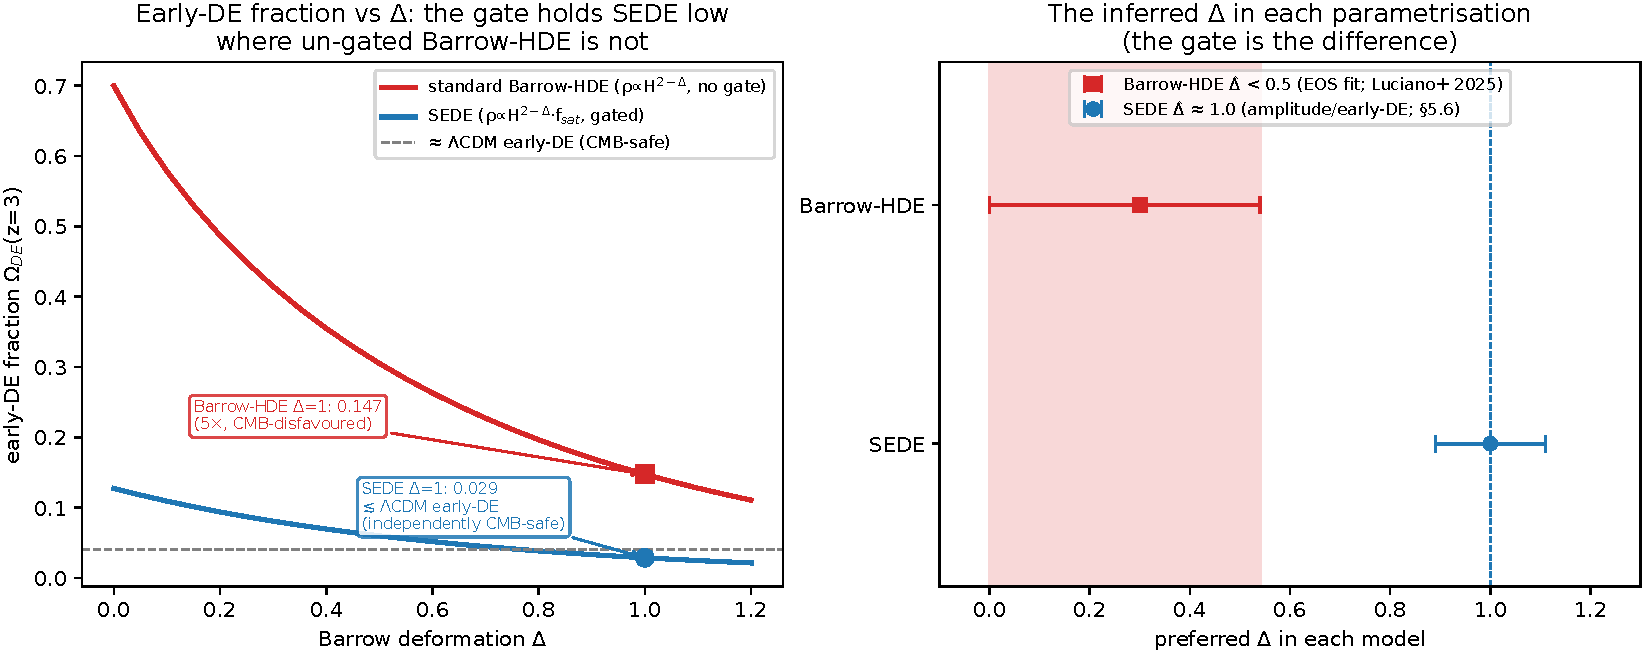
\includegraphics[keepaspectratio]{../../results/fig_delta_orthogonality}}
\caption{Why the standard Barrow-HDE bound \(\Delta \ll 1\) does not
constrain SEDE's \(\Delta = 1\). Both models share the holographic
scaling \(\rho _\mathrm{DE} \propto H^{2-\Delta }\); the only difference
is SEDE's structure gate \(f_{\mathrm{sat}}(z)\). \emph{Left:} the
early-dark-energy fraction \(\Omega _\mathrm{DE}(z=3)\) --- the quantity
the CMB and the standard-HDE EOS fit actually constrain --- versus
\(\Delta\). Un-gated Barrow-HDE (red) carries large, strongly
\(\Delta\)-dependent early DE \((\Omega _\mathrm{DE}(z=3) = 0.15\) even
at \(\Delta = 1\), rising to 0.70 at \(\Delta = 0\)), so its fits pin
\(\Delta < 0.5\); SEDE's gate (blue) drives \(f_{\mathrm{sat}}\) → 0 at
high z, holding \(\Omega _\mathrm{DE}(z=3) \approx 0.03\) --- at or
below the \(\Lambda \mathrm{CDM}/\mathrm{CMB}\)-safe level (grey dashed)
--- for \emph{all} \(\Delta\). At \(\Delta = 1\) the two models differ
five-fold (0.029 vs 0.147), and SEDE additionally crosses \(w = -1\)
\((w_{0} = -1.0)\) where un-gated Barrow-HDE does not
\((w_{0} = -0.77)\). \emph{Right:} consequently the data prefer
orthogonal \(\Delta\) in the two parametrisations --- \(\hat{\Delta}\)
\textless{} 0.5 for Barrow-HDE (EOS/early-DE;
{[}\citep{Luciano:2025elo}{]}) and \(\hat{\Delta}\) ≈ 1.0 for SEDE
(amplitude/early-DE; §\ref{sec-5-6}) --- with no contradiction. The gate
is the difference.}\label{fig:10}
\end{figure}

Net: the two threats that targeted the model itself (full-CMB tension;
the Barrow-\(\Delta\) bound) are answered by direct tests or a stated
model distinction; the two that target the \emph{context}
(birefringence; the low-z SN systematic) are real and partially outside
SEDE's control --- birefringence especially.

\textbf{Evidential status.} SEDE is a falsifiable, fixed-parameter,
\(\Lambda\)-free alternative to \(\Lambda \mathrm{CDM}\), moderately
preferred (calibrated p \textless{} 0.0015, 0/2000; ∼2--\(3\sigma\)
across pipelines) with an encouraging out-of-sample check, resting on
one open postulate and a few stated theoretical choices. It is stronger
than ``indistinguishable from \(\Lambda \mathrm{CDM}\)'' and weaker than
``established.'' Its value is twofold: a \emph{physical story} (no
fine-tuned \(\Lambda\), w(z) from \(\Omega _{\mathrm{m}}\), the
coincidence reframed) and a \emph{decidable prediction} (the volume law,
\(\Delta  = 1\)). The data, not the theory, will settle it.

\section{Conclusions}\label{sec-10}

We have presented Structural Entropy Dark Energy: a fixed-parameter
dark-energy model in which dark energy is identified with the conjugate
thermal energy density of a volume-law-entangled cosmic horizon and
activated through a structure-growth gate. The model is a single
Friedmann fixed-point equation with no fitted dark-sector parameter ---
\(\lambda\), w(z), \(\gamma\), and \(c_{\mathrm{s}}^{2}\) are each fixed
by a stated theoretical choice rather than tuned --- that replaces the
cosmological constant by a structure-gated, horizon-coupled term. It
addresses the vacuum-energy-scale problem (the scale is the CKN
holographic bound, normalised by flatness, not the QFT vacuum) and
reframes the \emph{timing} of the coincidence problem (the activation
gate tracks the late-time maturation of the structure-growth history);
it does not explain the present-day dark-energy \emph{magnitude}, which
--- as \(\rho _\mathrm{DE}\) ∼ \(M_{\mathrm{P}}^{2}H_{0}^{2}\) is
numerically the same coincidence --- it shares with \(\Lambda\). In a
marginalised, CAMB-in-the-loop joint analysis it is moderately preferred
over \(\Lambda \mathrm{CDM}\) \((\Delta \mathrm{DIC} \approx  -3.5\) to
\(-4.7\)); the preference is calibrated at p \textless{} 0.0015 (0/2000;
∼2--\(3\sigma\) across pipelines; not obviously flexibility) with an
encouraging pre-DESI → DESI out-of-sample check, and its equation of
state crosses \(-1\) in DESI's evolving-DE quadrant (∼\(0.5\sigma\) from
\(\Lambda \mathrm{CDM}\), so disfavoured alongside it if the steep DESI
signal firms up). On the growth side the completed perturbation sector
\emph{raises} late-time structure \((\sigma 8 \approx  0.811\) vs
0.800), so we make no claim on the S8 tension. Its quantum-gravitational
content reduces to one falsifiable postulate --- a volume-law horizon
entropy. The sharp future test is near: under the stated Fisher
assumptions, DESI DR3 and Euclid could constrain the effective
deformation \(\Delta\) to \(\sigma  \approx  0.09\), separating SEDE's
volume-law horizon from a smooth one at a nominal ∼\(11\sigma\) --- a
Fisher-optimistic figure; the honest framing is a discrete
\(\Delta  = 1\) versus \(\Delta  = 0\) model-selection test. SEDE is a
moderate preference, not established --- and, crucially, it is
decidable.

\section*{Data availability
statement}\label{data-availability-statement}
\addcontentsline{toc}{section}{Data availability statement}

The code, data vectors, and analysis pipelines that support the findings
of this study are openly available at
\url{https://github.com/spsingularity/sede-cosmology}, with a tagged
release archived at Zenodo, DOI
\href{https://doi.org/10.5281/zenodo.21525525}{10.5281/zenodo.21525525}.
The repository ships the model package (the background E(z), w(z), the
structure gate \(f_{\mathrm{sat}}\), and the halo-binding \(\gamma\)
derivation), the public data vectors, the figure generators, and the
\textbf{CAMB-in-the-loop inferential pipeline} --- the canonical
\((\lambda  = 1/2)\) background →
\(r_{\mathrm{drag}}/r_{\mathrm{star}}\) → BAO + compressed-CMB joint
likelihood, the marginalised MCMC \((\Delta \mathrm{DIC}\),
\(p_{\mathrm{D}}\)), the per-probe decomposition, the false-preference
mock calibration (Fig. 6), the out-of-sample split, the
\(tracer/\gamma\) robustness scans, and the sha256-locked prediction set
(\texttt{predictions.json}, verified byte-for-byte by
\texttt{gen\_predictions.py}). A single entry point
(\texttt{reproduce\_figures.py}) regenerates the figures, and the
inference drivers under \texttt{src/experiments/} regenerate the
headline model-comparison numbers; an automated verification suite
checks the background layer numerically. Two components are \emph{not}
regenerated locally and are reported from the companion
observational-tests analysis \citep{Pandev:2026obstest}: the
full-primary-CMB (plik) joint \((\Delta \mathrm{DIC} = -3.5\), robust
part \(\Delta\)⟨\(\chi ^{2}\)⟩ ≈ −3.0, eroded to \(-2.3\) by the
companion's direct Planck-lensing \(\phi \phi\) test; this paper's own
fold-in \(\Delta \chi ^{2} = -3.17\)), which needs the Planck likelihood
data, and the FPAB-SEDE cubic-KGB / Mochi-CLASS growth sector
\((\sigma 8\), \(\mu _\infty\), the ISW ratio, gravitational slip); the
nested-sampling evidence is reported via a Laplace estimate here (full
dynesty run in the companion). The observational inputs are third-party
public datasets (DESI DR2, Pantheon+/DES-5YR/Union3, Moresco cosmic
chronometers, Gold-2018 \(f\sigma 8\), compressed Planck, eBOSS DR16),
available at their cited original sources and retrieved via the
documented loaders.

\section*{Acknowledgements}\label{acknowledgements}
\addcontentsline{toc}{section}{Acknowledgements}

This research received no external funding, and the author --- an
independent researcher --- declares no competing interests. As sole
author, S. Pandev conceived the model, performed and independently
verified all analyses, and wrote the manuscript, taking full
responsibility for its content. Artificial-intelligence tools (large
language models) assisted with drafting and editing the manuscript,
developing and cross-checking the analysis code, and literature
searches; no AI tool is an author.

\appendix

\section{Key results, prescriptions, and assumptions}\label{sec-A}

This appendix documents the six load-bearing items, labelled by their
actual epistemic status --- one defining ansatz (A.1), supporting
derivations (A.2, A.4, A.5), a fixed prescription (A.3), and a motivated
postulate (A.6). The headings give that status; the parenthetical
``Result/Prescription/ Motivation N'' numbering corresponds to the
repository's theorem labels (retained there for code stability,
\emph{not} a claim that each is a mathematical theorem). We work in
units \(c = \hbar  = k_{\mathrm{B}} = 1\) and write
\(8\pi G = 1/M_{\mathrm{P}}^{2}\). The source statements are Results 1,
3, 4C, 5, 8, 9; the remaining items (2, 4, 4B, 6, 6B, 10--13, 5D) are
catalogued at the end with one-line statements.

\subsection{\texorpdfstring{The conjugate horizon-fluid ansatz:
\(\rho _\mathrm{DE} = T_\mathrm{AH}\cdot s_{\mathrm{grav}}\)}{The conjugate horizon-fluid ansatz: \textbackslash rho \_\textbackslash mathrm\{DE\} = T\_\textbackslash mathrm\{AH\}\textbackslash cdot s\_\{\textbackslash mathrm\{grav\}\}}}\label{sec-A-1}

\textbf{Claim.} SEDE \emph{identifies} the dark-energy density with the
conjugate energy of the horizon entropy,
\(\rho _\mathrm{DE} = T_\mathrm{AH}\cdot s_{\mathrm{grav}}\cdot f_{\mathrm{sat}}\),
with \(s_{\mathrm{grav}}\) the (volume-law) horizon entropy density and
\(f_{\mathrm{sat}} \in  [0\),1{]}. The Clausius relation supplies the
\emph{dynamics}; the absolute density \(\rho  = T\cdot s\) is the
model's defining ansatz, motivated by horizon thermodynamics --- not a
theorem.

\textbf{Setup.} At the flat-FRW apparent horizon
\(R_\mathrm{AH} = 1/H\), the dynamical Cai--Kim temperature is
\(T_\mathrm{AH} = (H/2\pi )(1 - \epsilon /2)\),
\(\epsilon\)≡−Ḣ/\(H^{2}\). We adopt the Gibbons--Hawking limit
\(T_\mathrm{AH} = H/2\pi\) \((\epsilon\) → 0), the leading temperature
appropriate for the de Sitter-attractor dark-energy sector; the
dynamical \((1 - \epsilon /2)\) correction is sub-leading where dark
energy matters and is disfavoured in full (§\ref{sec-2}, §\ref{sec-6}),
so it does not enter the calibrated E(z). The gravitational entropy is
the coarse-grained entanglement entropy in the horizon volume,
\(S_{\mathrm{grav}} \propto  V_\mathrm{AH} \propto  R_\mathrm{AH}^{3}\)
(§\ref{sec-3-3}, §\ref{sec-8-1}), i.e.~a \emph{constant} entropy density
\(s_{\mathrm{grav}} = s_{0}\) (in contrast to the Bekenstein--Hawking
area-law density \(s_\mathrm{AH}\)=¾\(M_{\mathrm{P}}^{2}H \propto  H\),
which would instead give the area-law model
\(\rho _\mathrm{DE} \propto  H^{2}\) --- the branch disfavoured in the
conditional diagnostics of §\ref{sec-5-6}).

\textbf{Construction.} \emph{Step 1 (Clausius --- the rigorous,
dynamical content).} Hayward's first law for a dynamical horizon,
\(\delta E = T_\mathrm{AH}\) \(dS_\mathrm{AH} + W\) \(\delta V\) with
work density \(W = (\rho  - p)/2\), applied to a shell of matter
crossing the horizon in time dt with flux \(-dE = (\rho  + p)H\) V dt,
gives the Clausius relation \((\rho  + p)H\) \(V = T_\mathrm{AH}\)
Ṡ\_AH. This relates \emph{changes} and is standard horizon
thermodynamics.

\emph{Step 2 (Bousso bound as motivation for a bounded
\(f_{\mathrm{sat}}\)).} The covariant entropy bound gives
\(S_{\mathrm{matter}} \leq  A/(4l_{\mathrm{P}}^{2}) = S_\mathrm{AH}\) on
any light-sheet bounded by the horizon. This \emph{motivates}
interpreting \(f_{\mathrm{sat}}\) as a bounded effective saturation
fraction; in SEDE we impose \(0 \leq  f_{\mathrm{sat}} \leq  1\) and
\(f_{\mathrm{sat}}(0) = 1\) with the redshift dependence supplied by the
halo prescription (A.2/A.3), and we do not identify \(f_{\mathrm{sat}}\)
literally with \(S_{\mathrm{matter}}/S_\mathrm{AH}\) (consistent with
the small binding-entropy budget, Appendix~\ref{sec-F}).

\emph{Step 3 (the SEDE identification --- the ansatz).} SEDE posits the
dark-energy density to be the conjugate energy of the volume-law horizon
entropy,
\begin{equation}\rho_{\rm DE} \equiv T_{AH}\,s_{\rm grav}\,f_{\rm sat} = \frac{H}{2\pi}\,s_0\,f_{\rm sat} \;\propto\; H\,f_{\rm sat}.\end{equation}
Fixing the one constant \(s_{0}\) by spatial flatness
\([\rho _\mathrm{DE}(0) = \Omega _\mathrm{DE}0\)
\(\rho _{\mathrm{crit}}\),0, \(f_{\mathrm{sat}}(0) = 1\){]} gives
\begin{equation}\rho_{\rm DE}(z) = \Omega_{\rm DE0}\,\rho_{\rm crit,0}\,\frac{H}{H_0}\,f_{\rm sat}(z)
= \Omega_{\rm DE0}\,\rho_{\rm crit,0}\,E(z)\,f_{\rm sat}(z),\end{equation} i.e.~the
fixed-point term \(\Omega _\mathrm{DE}0\cdot E\cdot f_{\mathrm{sat}}\)
of the boxed closure equation (§\ref{sec-2}) --- the volume-law
\((\lambda  = 1/2)\) scaling, \emph{not} the area-law \(H^{2}\). This is
an identification motivated by horizon thermodynamics, not a derivation:
the Clausius relation (Step 1) fixes the dynamics, while the absolute
density is the postulate (§\ref{sec-8-4}).

\emph{Step 4 (scale / coincidence).} \(\rho _\mathrm{DE}\) ∼
\(M_{\mathrm{P}}^{2}H_{0}^{2}\) ∼ \((10^{-3}\) \(eV)^{4}\) is small
because \(H_{0}/M_{\mathrm{P}}\) ∼ \(10^{-61}\). The CKN bound
(§\ref{sec-8-2}) \emph{explains} why this horizon scale is
∼\(\rho _{\mathrm{crit}}\) --- as an upper bound, taken here to be
saturated to O(1) by the flatness normalisation above --- replacing the
QFT-vacuum conflation behind the \(10^{120}\) problem rather than
deriving the magnitude from scratch. ∎

\subsection{\texorpdfstring{Result 3 --- the structure gate
\(f_{\mathrm{sat}}(z)\)}{Result 3 --- the structure gate f\_\{\textbackslash mathrm\{sat\}\}(z)}}\label{sec-A-2}

\textbf{Claim.}
\(f_{\mathrm{sat}}(z) = [1 - e^{-\gamma  x(z)}]/[1 - e^{-\gamma }]\),
where \(x \equiv  \sigma 8^{2}(z)/\sigma 8^{2}(0) = D^{2}(z)\) (D the
linear growth factor, D(0) = 1).

\textbf{Setup.} We model the cumulative activation gate directly
(dimensionless, avoiding any mix of area- and volume-law densities)
through a normalised growth-weighted deposition kernel
\(K(t) \propto  (d\sigma 8^{2}/dt)\)
\(e^{-\gamma \sigma 8^{2}/\sigma 8^{2}(0)}\) --- the structure-growth
rate \(d\sigma 8^{2}/dt > 0\) times a Boltzmann factor \(e^{-\gamma x}\)
for the exponential rarity of massive halos \((\gamma\) from A.3) ---
taking \(f_{\mathrm{sat}}\) to be its normalised cumulative from early
times to epoch z (cosmic time t),
\begin{equation}f_{\rm sat}(z) = \frac{\int_0^{t(z)} K\,dt}{\int_0^{t_0} K\,dt},\end{equation} so
that \(f_{\mathrm{sat}}(\infty ) = 0\) (early, t→0) and
\(f_{\mathrm{sat}}(0) = 1\) (today, \(t = t_{0}\)) by construction (the
closed-form gate below is this cumulative-kernel form, not a relaxation
ODE).

\textbf{Proof.} The kernel integrated over cosmic time is K dt
\(= (d\sigma 8^{2}/dt)\) \(e^{-\gamma \sigma 8^{2}/\sigma 8^{2}(0)}\) dt
= \(e^{-\gamma u}\) \(d\sigma 8^{2}\) with
\(u \equiv  \sigma 8^{2}/\sigma 8^{2}(0)\); the Hubble factors cancel
and the integral reduces to one over u. With u running from 0 (z′→∞, no
early structure) to
\(x(z) \equiv  \sigma 8^{2}(z)/\sigma 8^{2}(0) = D^{2}(z)\),
\begin{equation}f_{\rm sat}(z) = \frac{\int_0^{x(z)} e^{-\gamma u}\,du}{\int_0^{1} e^{-\gamma u}\,du}
= \frac{1 - e^{-\gamma x(z)}}{1 - e^{-\gamma}}, \qquad x(z) = D^2(z),\end{equation}
where the denominator (x = 1, i.e.~z = 0) enforces
\(f_{\mathrm{sat}}(0) = 1\). Checks: \(f_{\mathrm{sat}}(0) = 1\);
\(f_{\mathrm{sat}}(z \gg  1)\) → 0 as x → 0;
\(f_{\mathrm{sat}} \in  [0\),1{]} for \(x \in  [0\),1{]}. The form is
the CDF of a truncated exponential of rate \(\gamma\) on
\(x \in  [0\),1{]} --- the normalised activation fraction reached by
epoch z. ∎

\subsection{\texorpdfstring{Prescription 4C --- the fixed structure
coupling
\(\gamma  \approx  1.496\)}{Prescription 4C --- the fixed structure coupling \textbackslash gamma  \textbackslash approx  1.496}}\label{sec-A-3}

\textbf{Claim.} The entropy weight exponent is p = 5/3, giving
\(\gamma  = d\) ln \(\Sigma _{\mathrm{S}}^{(5/3)}/d\) ln
\(\sigma 8^{2} = 1.496\) (the derivative is w.r.t. the variance
\(\sigma 8^{2}\), the gate argument
\(x = D^{2} = \sigma 8^{2}/\sigma 8^{2}(0)\) of A.2; equivalently ½ d ln
\(\Sigma _{\mathrm{S}}/d\) ln \(\sigma 8 = 1.496\), i.e.~d ln
\(\Sigma _{\mathrm{S}}/d\) ln \(\sigma 8 = 2.993\)). A self-similar
reduction gives the closed form
\(\gamma  = (p-1)\)⟨\(1/\alpha\)⟩\_\(\Sigma\) with
\(\alpha  \equiv  -d\) ln \(\sigma /d\) ln M the effective spectral
slope over the entropy-weighted mass range; it reproduces the exact
mass-function integral to 0.1\% (the binding-energy companion note, §7).
Entropy is deposited by the \(\nu _{\mathrm{S}} \approx  2.4\)
(∼\(2\sigma\)) clusters at \(M_{\mathrm{S}}\) ∼ \(10^{14}\cdot ^{5}\)
\(M\odot /h\), giving an independent cluster-abundance handle; p = 1
gives \(\approx  0.27\) (∼\(5\times\) below p = 5/3), a weak gate versus
the real one.

\textbf{Proof.} In the SEDE horizon-fluid ansatz (A.1),
\(f_{\mathrm{sat}}\) is the effective fraction of the cosmic-horizon
entropy capacity that is gravitationally activated, and
\(\rho _\mathrm{DE} = T_\mathrm{AH}\cdot s_{\mathrm{grav}}\cdot f_{\mathrm{sat}}\)
--- so the entropy that defines the \(f_{\mathrm{sat}}\) weighting is
accounted in the \emph{horizon} reservoir at the \emph{horizon}
temperature \(T_\mathrm{AH} = H/2\pi\). By Clausius, heat Q deposited
into a reservoir at temperature T adds entropy Q/T. When a halo of mass
M virialises it releases gravitational binding energy
\(E_{\mathrm{bind}} \propto  M^{5/3}\) (NFW;
\(R_{\mathrm{vir}} \propto  M^{1/3}\); verified slope 1.64). Under the
SEDE prescription this released binding energy is accounted in the
horizon entropy ledger at the horizon temperature \(T_\mathrm{AH}\) (we
do not claim a demonstrated transport mechanism), so the entropy
assigned in this ledger is
\begin{equation}\Delta S_{AH} = \frac{E_{\rm bind}}{T_{AH}} \propto \frac{M^{5/3}}{H}.\end{equation}
Because \(T_\mathrm{AH} \propto  H\) is identical for every halo at a
given epoch (mass-independent), the per-halo mass weight is \(M^{5/3}\):
p = 5/3. With \(\Sigma _{\mathrm{S}}\)=∫ \(M^{5/3}(dn/d\) ln M)d ln M
and a Sheth--Tormen mass function (COLOSSUS, EH98 transfer,
\(M \in  [10^{10}\), \(10^{16}\){]} \(M_\odot\)),
\begin{equation}\gamma = \frac{d\ln\Sigma_S^{(5/3)}}{d\ln\sigma_8^2} = \tfrac{1}{2}\,\frac{d\ln\Sigma_S^{(5/3)}}{d\ln\sigma_8} = 1.4964 \approx 1.50\end{equation}
(the derivative is w.r.t. the variance \(\sigma 8^{2}\) because the
gate's argument is \(x = D^{2} = \sigma 8^{2}/\sigma 8^{2}(0)\);
equivalently d ln \(\Sigma _{\mathrm{S}}/d\) ln \(\sigma 8 = 2.993\)).
The earlier p = 1 (Result 4B) divided \(E_{\mathrm{bind}}\) by the
\emph{halo's} virial temperature \(T_{\mathrm{vir}} \propto  M^{2/3}\),
which is the entropy of the halo's own internal state --- correct for
the halo, wrong for the entropy added to the cosmic horizon (where
\(f_{\mathrm{sat}}\) lives). The heat is the same; the reservoir, and
hence the temperature, is the horizon's. ∎

\subsection{\texorpdfstring{Result 5 --- the structural-EOS diagnostic
(the \(w_{0}\) side-note, not canonical
w(z))}{Result 5 --- the structural-EOS diagnostic (the w\_\{0\} side-note, not canonical w(z))}}\label{sec-A-4}

\textbf{Claim (structural EOS).}
\(w_{\mathrm{struct}}(0) = -1 + \gamma /[3(e^{\gamma } - 1)]\),
well-approximated by the closed-form algebraic expression
\(w_{\mathrm{alg}} = (4\Omega _{\mathrm{m}}/3 - 1)/(1 - \Omega _{\mathrm{m}})\).
(This is the side-note structural estimate of §\ref{sec-3-2}, not the
model's prediction, which is the canonical crossing w(z).)

\textbf{Proof.} From \(\rho _\mathrm{DE}(z) = \rho _{\mathrm{crit}}\),0
\(\Omega _\mathrm{DE}0\) \(f_{\mathrm{sat}}(z)\) (A.1) with
\(f_{\mathrm{sat}}(x)\), \(x = D^{2}\), the structural EOS in the
variance variable is \(w_{\mathrm{struct}}(0) = -1 + (1/3)\)
\(df_{\mathrm{sat}}/dx\)\textbar\_\{x=1\}. Differentiating the Result-3
form,
\begin{equation}\left.\frac{df_{\rm sat}}{dx}\right|_{x=1} = \frac{\gamma e^{-\gamma}}{1 - e^{-\gamma}} = \frac{\gamma}{e^\gamma - 1},\end{equation}
so \(w_{\mathrm{struct}}(0) = -1 + \gamma /[3(e^{\gamma } - 1)]\). At
\(\gamma  = 1.4964\) this is 0.432, giving
\(w_{\mathrm{struct}}(0) = -0.856\) \((0.33\sigma\) from DESI DR2).
Numerically
\(\gamma /(e^{\gamma } - 1) = 0.432 \approx  \Omega _{\mathrm{m}}/(1 - \Omega _{\mathrm{m}}) = 0.451\)
at the observed parameters, so the structural value is approximated to
∼4\% by the closed-form expression
\(w_{\mathrm{alg}} = (4\Omega _{\mathrm{m}}/3 - 1)/(1 - \Omega _{\mathrm{m}}) = -0.849\)
\((0.21\sigma\) from DESI). This is a numerical approximation in the
\(x = D^{2}\) convention, not an exact identity. (The interacting-fluid
effective EOS, from Raychaudhuri + Friedmann at z = 0, is phantom,
\(w_{\mathrm{fluid}}(0) \approx  -1.15\), because \(f_{\mathrm{sat}}\)
is still rising today; the canonical \(\lambda  = 1/2\) background
realises this as a crossing of \(-1\), §\ref{sec-5-1}.) ∎

\subsection{\texorpdfstring{Result 8 --- the H-coupling
\(\lambda  = 1 - \Delta /2\)}{Result 8 --- the H-coupling \textbackslash lambda  = 1 - \textbackslash Delta /2}}\label{sec-A-5}

\textbf{Claim.} With the Barrow entropy \(S = (A/A_{0})^{1+\Delta /2}\),
the conjugate horizon-fluid ansatz gives
\(\rho _\mathrm{DE} \propto  H^{2\lambda }\) \(f_{\mathrm{sat}}\) with
\(\lambda  = 1 - \Delta /2\).

\textbf{Proof.} A quantum-gravitationally rough horizon carries the
Barrow entropy \(S = (A/A_{0})^{1+\Delta /2}\),
\(\Delta  \in  [0\),1{]}, in place of the area law. With
\(A = 4\pi /H^{2}\) and \(V_\mathrm{AH} \propto  H^{-3}\), the
Barrow-deformed entropy density (written \(s_\Delta\) to distinguish it
from the Bekenstein--Hawking area-law density
\(s_\mathrm{AH} \propto  H\)) is
\begin{equation}s_{\Delta} = \frac{S}{V_{AH}} \propto \frac{(H^{-2})^{1+\Delta/2}}{H^{-3}} = H^{1-\Delta},\end{equation}
\begin{equation}\rho_{\rm DE} = T_{AH}\,s_{\Delta}\,f_{\rm sat} \propto H\cdot H^{1-\Delta}\cdot f_{\rm sat}
= H^{2-\Delta}f_{\rm sat} \equiv H^{2\lambda}f_{\rm sat}, \qquad \boxed{\lambda = 1 - \tfrac{\Delta}{2}.}\end{equation}
This is Barrow holographic dark energy with the Hubble IR cutoff
\((\rho _\mathrm{DE} \propto  L^{\Delta -2}\), L = 1/H). The endpoints
are \(\Delta  = 0\) ⟹ \(\lambda  = 1\) (the area-law branch,
disfavoured) and \(\Delta  = 1\) ⟹ \(\lambda  = 1/2\) (the volume-law
postulate, A.6). \(\lambda\) is therefore not a free parameter; it is
set by the Barrow deformation. \textbf{Scope:} the Barrow exponent
multiplies only the \(f_{\mathrm{sat}}\)-gated \(\rho _\mathrm{DE}\),
\emph{not} the gravitational sector, so H(z) at BBN equals the standard
matter+radiation value to ∼8 figures
\((\Omega _\mathrm{DE}/\rho _{\mathrm{tot}}\) ∼ \(10^{-16}\) at z ∼
\(4\times 10^{9}\)); the modified-gravity BBN bound
\(\Delta  \lesssim  10^{-4}\) does not apply, and constant
\(\Delta  = 1\) is BBN-safe. ∎

\subsection{\texorpdfstring{Motivation 9 --- \(\Delta  = 1\) from a
geometric ceiling and the
GSL}{Motivation 9 --- \textbackslash Delta  = 1 from a geometric ceiling and the GSL}}\label{sec-A-6}

\textbf{Claim.} \(\Delta  = 1\) (the volume-law endpoint) is
\emph{strongly motivated} --- not fitted to cosmological data --- by two
independent principles; it is the central postulate (§\ref{sec-8-4}),
not a microscopic derivation.

Pillar 1 --- geometric ceiling. The Barrow deformation is the fractal
(Hausdorff) dimension of the horizon surface,
\(d_{\mathrm{H}} = 2 + \Delta\). A 2-surface embedded in 3-space cannot
exceed the space-filling dimension \(d_{\mathrm{H}} = 3\), so
\(\Delta  \leq  1\), with \(\Delta  = 1\) the extremum where the
area-measure becomes a volume-measure
\((S \propto  A^{3/2} \propto  R^{3})\). This is Barrow's defining
range. \emph{(Superseded, not withdrawn: the count companion paper
\citep{Pandev:2026count} derives the same ceiling \(\Delta  \leq  1\) as
a theorem from a finite per-site leg budget,
\(C \leq  \kappa \cdot\)\textbar{}\(\Omega\)\textbar, and shows the
count is not literally a Hausdorff dimension --- so the fractal picture
here is a heuristic for a bound that now has a stronger, premise-free
proof.)}

Pillar 2 --- thermodynamic attractor. Three premises: (P1) the DE sector
is purely entropic --- SEDE posits \(\rho _\mathrm{DE} = T_\mathrm{AH}\)
\(s_{\mathrm{grav}}\), so the free-energy density
\(F = \rho _\mathrm{DE} - T_\mathrm{AH}\) \(s_{\mathrm{grav}} = 0\)
identically; the governing potential is therefore the \emph{entropy},
not \(F = E - \mathrm{TS}\) (this is the load-bearing step: with a
nonzero \(\Delta\)-dependent free energy, equilibrium would extremise F
and \(\Delta  = 1\) would not follow). (P2) the generalised second law:
\(S_{\mathrm{total}} = S_\Delta  + S_{\mathrm{matter}}\) is
non-decreasing, \(S_{\mathrm{matter}}\) independent of \(\Delta\). (P3)
\(\Delta\) is a thermalising horizon degree of freedom (the standard
Jacobson--Padmanabhan assumption). By (P1)--(P2), maximising
\(S_{\mathrm{total}}\) over \(\Delta\) reduces to maximising
\(S_\Delta  = (A/A_{0})^{1+\Delta /2}\), whose derivative is
\begin{equation}\frac{dS_\Delta}{d\Delta} = \frac{S_\Delta}{2}\ln\!\frac{A}{A_0} + [\text{back-reaction through }A(\Delta)].\end{equation}
The explicit term carries
\(ln(A/A_{0}) \approx  ln(10^{122}) \approx  280 > 0\) (a vastly
super-Planckian horizon). The back-reaction \((\Delta\) shifts
\(\rho _\mathrm{DE} \propto  H^{2-\Delta }\), hence H, hence A) cannot
flip the sign: it \emph{vanishes} at z = 0 \((H = H_{0}\) ⟹ ln H = 0 ⟹
\(\partial _\Delta\) \(H^{2-\Delta } = 0\)) and is ∼1/280-suppressed
elsewhere. Hence \(dS_\Delta /d\Delta  > 0\) on all of {[}0,1{]}; a
strictly increasing function on a closed interval attains its maximum at
the right endpoint. With the ceiling \(\Delta  \leq  1\) (Pillar 1) the
constrained maximum is uniquely \(\Delta  = 1\), and by (P3) a
thermalising horizon relaxes to it.

\textbf{Conclusion.} Under the additional assumptions that \(\Delta\) is
a thermalising horizon degree of freedom (P3) and that entropy
maximisation over the Barrow family is the correct variational principle
(P1), the GSL argument is a consistency check --- the endpoint
\(\Delta  = 1\) is a GSL \emph{fixed point} --- rather than a selection
principle: the geometric ceiling \(d_{\mathrm{H}} = 3\) supplies the
bound \(\Delta  \leq  1\), and saturation of that cap \emph{is} the
volume-law postulate in effective form (via \(\lambda  = 1 - \Delta /2\)
this gives \(\lambda  = 1/2\)). These assumptions motivate but do not
microscopically derive the endpoint (§\ref{sec-8-4}). Because
\(S_\Delta\) is monotone in \(\Delta\), the same argument favours
\(\Delta  = 1\) at all epochs (the adopted constant \(\Delta\)). The
current conditional diagnostics prefer values near
\(\Delta (0) \approx  1.0\)--1.1 (§\ref{sec-5-6}), consistent with the
endpoint. This is a strong motivation, not a derivation: it reduces
\(\Delta  = 1\) from a fitted coupling to a GSL-equilibrium extremum
under the stated premises, leaving the microscopic origin open. ∎

\subsection{The remaining repository items (catalogue)}\label{sec-A-7}

\textbf{Result 2} (reheating master equation): the same logistic
\(df_{\mathrm{sat}}/dt = H\)
\(f_{\mathrm{sat}}(1 - f_{\mathrm{sat}}) - \Gamma\) \(f_{\mathrm{sat}}\)
governs the \emph{early} \(f_{\mathrm{sat}}\) (inflaton→radiation),
giving the U-shape of Result 12. \textbf{Result 4 / 4B} {[}superseded by
4C{]}: the \(M^{5/3}\) energy weight, and the p = 1 virial-temperature
mis-step. \textbf{Result 5D}: the \((1 - \epsilon /2)\)
``\(\lambda  = 1\) variant'' background \((w_{0} = -0.85\), no crossing)
vs the canonical \(\lambda  = 1/2\) crossing background. \textbf{Result
6 / 6B}: the smooth-DE growth validation and the
\(c_{\mathrm{s}}^{2} = 1\) closure \((f_{\mathrm{sat}}\) a background
functional). \textbf{Result 10}: the QG chain and the volume-law
postulate. \textbf{Result 11}: the seam = BBN bound =
modgrav/holographic fork. \textbf{Result 12}: the \(f_{\mathrm{sat}}\)
U-shape (inflation and dark energy as the two de Sitter brackets).
\textbf{Result 13}: \(1 + w = (1/3)[2\lambda \epsilon  - d\) ln
\(f_{\mathrm{sat}}/d\) ln a{]}, the EOS as horizon-entropy production.
Full statements are catalogued here; each is exercised by a numbered
check in Appendix~\ref{sec-B}.

\section{The verification suite}\label{sec-B}

The accompanying code ships a suite of 63 numerical checks (V1--V63)
covering: the fixed-point solution (closed-loop H(z) to \(10^{-13}\)
over \(z \in  [0\), \(10^{6}\){]}), BBN-safety
\((\Delta N_{\mathrm{eff}} = \Delta Y_{\mathrm{p}} = 0)\), the
\(\mathrm{CAMB}\equiv \mathrm{CLASS}\) \(r_{\mathrm{drag}}\) agreement
\((5\times 10^{-5})\), the CLASS perturbation validation (0.1\%), the
GSL along cosmic history, the fixed (derived, Prescription 4C)
\(\gamma\) and the smooth-DE \(c_{\mathrm{s}}^{2} = 1\) closure, the
horizon-dimension scaling
\(\lambda (d_{\mathrm{H}}) = 2 - d_{\mathrm{H}}/2\) (V59), the
state/counting diagnostics of the supplementary material (§S2; SYK
scrambling V60; causal-set dof counting in Minkowski + de Sitter V61;
the entropy-bound audit V62; the tensor-network realisability test V63),
and the cross-horizon and quantum-sector consistency checks. The
verification suite and the figures regenerate from the repository, and
the CAMB-in-the-loop inference drivers under \texttt{src/experiments/}
regenerate the headline model-comparison numbers
\((\Delta \mathrm{DIC}\), the per-probe decomposition, the
false-preference calibration, the out-of-sample split, and the
\(tracer/\gamma\) robustness scans). Only the full-primary-CMB (plik)
joint and the FPAB/Mochi-CLASS growth sector are run by the companion
observational-tests analysis \citep{Pandev:2026obstest} (they need the
Planck likelihood data and the modified Boltzmann code respectively; see
the Data-availability statement).

\section{\texorpdfstring{Data vectors, covariances, and the
\(f\sigma 8\)
audit}{Data vectors, covariances, and the f\textbackslash sigma 8 audit}}\label{sec-C}

The full data vectors and covariance matrices, the positive-definiteness
checks, the benign Pantheon+ duplicate-CID treatment, and the
\(f\sigma 8\) data audit (the small set of mis-entered growth points
corrected to their published Gold-2018 \citep{Sagredo:2018ahx} values,
and the SH0ES value correction) --- all reproduced from the public data
vectors and documented in the data audit. One approximation is
disclosed: the Moresco cosmic-chronometer covariance is applied as a
diagonal + 3\% correlated-systematic floor (the full published
covariance is cached separately); the CC channel contributes only +0.10
to \(\Delta \chi ^{2}\) and removing it entirely shifts the headline by
\(\leq  0.1\), so the approximation is immaterial to the model
comparison.

\section{False-preference calibration methodology}\label{sec-D}

The parametric-bootstrap procedure of §\ref{sec-5-2}: generation of
\(\Lambda \mathrm{CDM}\)-truth mocks with all probes (including the
compressed CMB \(R/l_{\mathrm{A}}\) and SH0ES) re-drawn
self-consistently; the refit of both models to each mock; the null
distribution of
\(\Delta \chi ^{2}(\mathrm{SEDE} - \Lambda \mathrm{CDM})\) (2000-mock
run: mean +0.61, s.d. 1.59); the real \(\Delta \chi ^{2}=-4.68\) beyond
all draws, 0/2000, p \textless{} 0.0015 (∼\(3\sigma\)); the documented
bug (CMB held fixed → biased null \(-2.87\), \(p \approx  0.5\)) and its
fix; and the independent-pipeline cross-check (∼\(2\sigma\),
CMB-distance-engine-dependent; run against the pre-revision real value
\(-2.96\) and not yet repeated at \(-4.68\)). The pre-registration
sha256 and contents are listed. The pre-registration additionally
records the triggered CMB follow-ups and their status (§\ref{sec-E}:
full non-lite plik run, \(\Delta \chi ^{2}=-0.33\); ACT DR6 primary
formally deferred) and the locked E1 structure-sourcing decision rule
(§\ref{sec-F}: data vector + CONFIRM/REFUTE thresholds). The no-SH0ES
robustness (§\ref{sec-5-4} ii′; \(\Delta \chi ^{2}=-2.89\), ln
\(B\approx +1.4\), ∼\(2.3\sigma\)) is reproduced by the no-SH0ES
robustness check.

\section{Status of the QG derivation chain}\label{sec-E}

The full chain from §\ref{sec-8}, with the status of each link: -
Jacobson--Cai--Kim (motivational ansatz): Clausius horizon
thermodynamics motivates the horizon-fluid construction and supplies the
conservation/dynamical logic \((\delta Q = T\) dS ⟹ Friedmann); the
\emph{absolute} identification \(\rho _\mathrm{DE} = T\cdot s\) is the
SEDE ansatz (A.1), not a theorem. - Non-extensivity ⟹
Tsallis--Cirto/Barrow power law (motivated): the weakest step. -
Second-law / GSL ⟹ volume-law endpoint \(\Delta  = 1\) (motivated, given
the volume-law thermalisation premise): the geometric ceiling caps
\(\Delta  \leq  1\) and the GSL is \emph{consistent with} (a fixed point
at) the saturated endpoint --- a consistency check, not a selection
principle; a microscopic derivation remains open. - CKN scale (a
rigorous bound, normalised by flatness): the holographic energy bound
gives the horizon-scale upper bound; the amplitude is normalised by
flatness (§\ref{sec-8-2}). - The one irreducible postulate (open): a
microscopic state count delivering the volume law.

The perturbative-QG (log-correction) vs thermalised (volume-law) regimes
are reconciled as different \emph{states}, not a contradiction. This
summary matches §\ref{sec-8-4} and Appendix~\ref{sec-F}.

\section{The energy and entropy budget}\label{sec-F}

This appendix records the order-of-magnitude estimate that the
energy-conservation framing of §\ref{sec-1}--§\ref{sec-2} turns on, and
the resulting summary of what is derived, normalised, and open.

\textbf{Energy budget.} Dark energy today is \(\rho _\mathrm{DE}\)
\(c^{2} \approx  0.7\) \(\rho _{\mathrm{crit}}\)
\(c^{2} \approx  6\times 10^{-10}\) \(J/m^{3}\). The gravitational
binding energy released by structure is bounded by
\textbar{}\(E_{\mathrm{bind}}\)\textbar/\(Mc^{2}\) ∼
\(\sigma ^{2}/c^{2}\) per virialised system, with \(\sigma\) ∼
\(10^{3}\) km/s for clusters \((\sigma ^{2}/c^{2}\) ∼ \(10^{-5}\)) and
∼200 km/s for galaxies (∼\(10^{-7}\)); even taking all of
\(\Omega _{\mathrm{m}}\) collapsed, \(\rho _{\mathrm{bind}}\)
\(c^{2} \lesssim  10^{-5}\) · 0.3 · \(8.5\times 10^{-10}\) ∼
\(10^{-15}\) \(J/m^{3}\). Hence
\(\rho _{\mathrm{bind}}/\rho _\mathrm{DE}\) ∼ \(10^{-6}\): binding
energy is six orders of magnitude too small to \emph{be} the dark
energy. A literal matter→dark-energy transfer is excluded independently
--- moving \(O(\rho _{\mathrm{crit}})\) out of matter over a Hubble time
would spoil \(\rho _{\mathrm{m}} \propto  a^{-3}\) and with it BBN and
the CMB.

Entropy budget. Deposited at the cold horizon temperature, the binding
entropy is \(\Delta S_\mathrm{AH}\)=
\(E_{\mathrm{bind}}/T_\mathrm{AH}\); with
\(T_\mathrm{AH} = \hbar H/2\pi\) this comes to \(\Delta S_\mathrm{AH}\)
∼ \(10^{-7}\) \(S_\mathrm{AH}\), i.e.~∼\(10^{-7}\) of the horizon
entropy. So binding-entropy deposition does not, by itself, fill
\(f_{\mathrm{sat}}\) to O(1); it sets the \emph{relative} z-dependence
(the weight p = 5/3 → \(\gamma\)), while the normalisation
\(f_{\mathrm{sat}}(0) = 1\) is set by the horizon capacity. This is the
same family as the \((M_{\mathrm{P}}/H)^{\Delta }\) ∼ \(10^{61}\)
``seam'' (Result 11), resolved by the holographic-DE scope (Barrow acts
only on the \(f_{\mathrm{sat}}\)-gated dark-energy fluid).

\textbf{Summary.}

\begin{longtable}[]{@{}
  >{\raggedright\arraybackslash}p{(\linewidth - 4\tabcolsep) * \real{0.3333}}
  >{\raggedright\arraybackslash}p{(\linewidth - 4\tabcolsep) * \real{0.3333}}
  >{\raggedright\arraybackslash}p{(\linewidth - 4\tabcolsep) * \real{0.3333}}@{}}
\toprule\noalign{}
\begin{minipage}[b]{\linewidth}\raggedright
quantity
\end{minipage} & \begin{minipage}[b]{\linewidth}\raggedright
status
\end{minipage} & \begin{minipage}[b]{\linewidth}\raggedright
set by
\end{minipage} \\
\midrule\noalign{}
\endhead
\bottomrule\noalign{}
\endlastfoot
magnitude \(\rho _\mathrm{DE}\) ∼ \(\rho _{\mathrm{crit}}\) & bounded +
normalised & CKN holographic upper bound (§\ref{sec-8-2}), amplitude
fixed by flatness (O(1) saturation of the bound assumed) \\
H-scaling \(\lambda  = 1/2\) & postulate & volume-law horizon entropy
\(S_{\mathrm{grav}} \propto  V_\mathrm{AH}\) (§\ref{sec-8-1}) \\
shape \(\gamma  \approx  1.5\) & derived (Prescription 4C) &
halo-binding-energy weighting \(E_{\mathrm{bind}} \propto  M^{5/3}\) → p
= 5/3 (§\ref{sec-3-1}) \\
sound speed \(c_{\mathrm{s}}^{2} = 1\) & closure & minimal smooth-DE
treatment, \(f_{\mathrm{sat}}\) a background functional
(§\ref{sec-3-4}) \\
normalisation \(f_{\mathrm{sat}}(0) = 1\) & imposed & present-day
horizon-entropy normalisation \\
volume-law horizon \((\Delta  = 1\) microscopically) & open & the one
irreducible postulate (§\ref{sec-8-4}) \\
\end{longtable}

None of these is a parameter \emph{fitted to cosmological data}, but
neither are they all ``derived from first principles'' --- the magnitude
is a holographic bound normalised by flatness (as
\(\Lambda \mathrm{CDM}\) normalises \(\Omega _\Lambda 0\)), the
H-scaling is the central volume-law postulate, \(\gamma\) is a fixed
halo prescription, and \(c_{\mathrm{s}}^{2} = 1\) is a modelling
closure. Binding energy enters SEDE entropically, fixing the
\emph{shape} of the gate; the dark energy's \emph{magnitude} is the
horizon's own thermal scale, not energy borrowed from structure. The
single irreducible foundational input is the microscopic volume-law
postulate.
\bibliographystyle{JHEP}
\bibliography{refs}
\end{document}
